% Front matter #######################################################
\frontmatter

% Page de garde

\includepdf[pages=-]{assets/couverture_these.pdf}

% Customize header and footer
\fancypagestyle{plain}{%  the preset of fancyhdr
    \fancyhf{} % clear all header and footer fields
    \fancyfoot[C]{\thepage} % except the center
    \renewcommand{\headrulewidth}{0pt}
    \renewcommand{\footrulewidth}{0pt}}
\pagestyle{fancy}
\fancyhf{}
\fancyhead[LE]{\leftmark}
\fancyhead[RO]{\rightmark}
\fancyhead[LO]{\today}
\fancyfoot[CE,CO]{\thepage}

\newcommand\Axel[1]{\textbf{\textcolor{red}{(A: #1)}}}

% Dédicaces
% \chapter*{Dedications}%
% Les dédicaces c'est par ici.


% Abstract
\chapter*{Abstract}
\small
\vspace{-1em}
\section*{Abstract}%
\label{sec:Abstract}

Computer vision is the computational science aiming at reproducing and improving
the ability of human vision to understand its environment.
In this thesis, we focus on two fields of computer vision, namely image segmentation
and visual odometry and
we show the positive impact that interactive Web applications provide on each.

The first part of this thesis focuses on image annotation and segmentation.
We introduce the image annotation problem
and challenges it brings for large, crowdsourced datasets.
Many interactions have been explored in the literature to help segmentation algorithms.
The most common consist in designating contours,
bounding boxes around objects,
or interior and exterior scribbles.
When crowdsourcing, annotation tasks are delegated
to a non-expert public, sometimes on cheaper devices such as tablets.
In this context, we conducted a user study showing
the advantages of the outlining interaction over scribbles and bounding boxes.
Another challenge of crowdsourcing is the distribution medium.
While evaluating an interaction in a small user study does not require complex setup,
distributing an annotation campaign to thousands of potential users might differ.
Thus we describe how the Elm programming language helped us
build a reliable image annotation Web application.
A highlights tour of its functionalities and architecture is provided,
as well as a guide on how to deploy it to crowdsourcing services
such as Amazon Mechanical Turk.
The application is completely open source and available online.

In the second part of this thesis we present our open source
direct visual odometry library.
In that endeavor, we provide an evaluation of other open source
RGB-D camera tracking algorithms and show that our approach
performs as well as the currently available alternatives.
The visual odometry problem relies on geometry tools and optimization techniques
traditionally requiring much processing power to perform at realtime framerates.
Since we aspire to run those algorithms directly in the browser,
we review past and present technologies
enabling high performance computations on the Web.
In particular, we detail how to target a new standard called WebAssembly from
the C++ and Rust programming languages.
Our library has been started from scratch in the Rust programming language,
which then allowed us to easily port it to WebAssembly.
Thanks to this property, we are able to showcase
a visual odometry Web application with multiple types of interactions available.
A timeline enables one-dimensional navigation along the video sequence.
Pairs of image points can picked on two 2D thumbnails
of the image sequence to realign cameras and correct drifts.
Colors are also used to identify parts of the 3D point cloud,
selectable to reinitialize camera positions.
Combining those interactions enables improvements
on the tracking and 3D point reconstruction results.

\normalsize

% Table des matières
\dominitoc%
\tableofcontents

% Main matter ########################################################
\mainmatter%

% Set style of code blocks throughout the document
\lstset{style=CodeStyle}

\chapter*{Introduction}%
\label{cha:introduction}
\addcontentsline{toc}{chapter}{Introduction}
Computer vision is the computational science aiming at reproducing and improving
the ability of human vision to understand its environment from light sensors.
Throughout a somewhat unconventional, multidisciplinary journey,
this document aims at answering the following question.
How can we leverage user interactions and the Web platform to improve
fields of computer vision such as image segmentation and visual odometry.

On the one hand, image segmentation (cf Figure~\ref{fig:segmentation})
is the task of identifying precise regions
in an image that are structurally or semantically different.
For medical images, it could be localizing cancer cells while
for urban images, differenciating people, vehicles and traffic signs.
On the other hand, visual odometry consists in analyzing the video stream of a sensor
such as a camera to locate and track its trajectory with regard to its environment
(cf Figure~\ref{fig:visual-odometry}).

\begin{figure}[h]
	\centering
	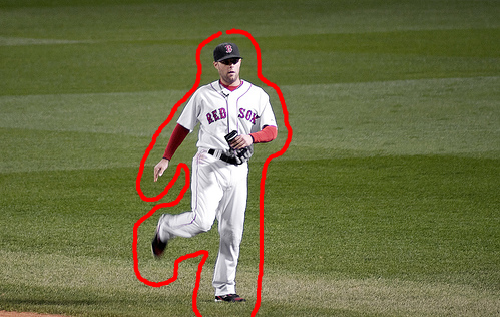
\includegraphics[width=0.45\linewidth]{assets/img/segmentation-interaction.png}
	\hfill
	
\includegraphics[width=0.45\linewidth]{assets/img/segmentation-mask.png}
	\caption{Outlining interaction in red and resulting segmentation mask.}%
	\label{fig:segmentation}
\end{figure}

\begin{figure}[h]
	\centering
	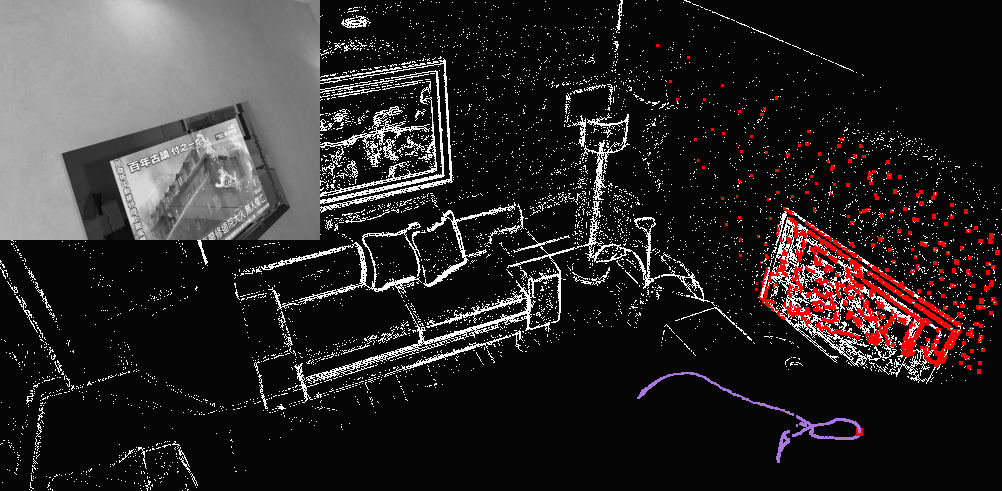
\includegraphics[width=\linewidth]{assets/img/visual-odometry.png}
	\caption{Camera trajectory (purple) and sparse 3D reconstruction
	generated by visual odometry.}%
	\label{fig:visual-odometry}
\end{figure}

Thanks to improvements in imaging and algorithms,
we are now able to automate tasks that were considered science-fiction until recently.
% Let's take self-driving cars as an example.
For instance, some companies~\cite{audia8} claim to have reached level 3
of SAE classification~\cite{sae-cars},
meaning that a self-driving vehicle provides autonomy at limited speed,
conditionned by locality and weather among other restrictions.
Nethertheless, we are still far from reaching level 5 of SAE classification
which requires full autonomy in any driving condition.
One non-technical reason is that owners of autonomous vehicles would be reluctant
to accept liability for potential accidents like the incident
of March 18, 2018, that killed Elaine Herzberg~\cite{elaineherzberg}.
I believe that such vehicles will only widespread when they are
safe enough for manufacturers to bear responsability of accidents.
Those capabilities depend on many research fields
including object detection and segmentation of urban images,
as well as visual odometry.
The former is required to detect the road, understand traffic signs,
avoid people, while the latter is needed to precisely record
the vehicle trajectory, especially in situations where other sensors
are not available or sufficiently precise, such as GPS in covered areas.

There exist many approaches for object detection and image segmentation.
Today, the ones performing best rely on a field of research named machine learning.
It consists in building prediction models by aggregating knowledge
from databases of pairs of inputs and outputs called learning datasets.
There are subtleties within the field
and not all algorithms perform equal but a general rule is that
the bigger and most accurate the learning dataset is,
the best will be the detection and segmentation results.
I will thus not focus on machine learning algorithms
but rather on the creation of those datasets.
That process is known as image annotation.
Annotating an image may take different forms depending on the task,
whether it is classification, object detection or segmentation.
In general, it consists in people using image manipulation tools
to draw rectangles, lines, polygons, and other geometric shapes
to identify regions of an image and assign it a label.
The Microsoft COCO dataset~\cite{lin2014microsoft} for example
contains 2.5 million labeled instances accross 328k images annotated by humans,
and required over 22 hours per thousand segmentations.
For a French worker, 35h a week, 228 day a year, this represents approximately 35 years,
almost a full career devoted to that single task.
It is thus understandable that building such datasets must be carefully thought of.

In the first part of this document I will focus on image annotation and segmentation.
Chapter~\ref{cha:the_image_annotation_problem} introduces in more details
the image annotation problem and challenges it brings for large, crowdsourced datasets.
In Chapter~\ref{cha:contribution_outlining}, we focus on the interactive segmentation task.
Many interactions have been explored in the literature to help segmentation algorithms.
The most common consist in designating contours~\cite{russell2008labelme},
bounding boxes around objects~\cite{rother_grabcut:_2004},
or interior and exterior scribbles~\cite{mcguinness2010comparative}.
Crowdsourcing such tasks however implies that non-expert users have to perform
those interactions and the distinction between expert and non-expert users is rarely touched.
Inspired by the work of Korinke et al.~\cite{korinke_intuitive_2015, korinke_exploring_2015},
we present a user study showing the advantages of the outlining interaction
for crowdsourcing annotations to a non-expert public.
This work has been published at ACM Multimedia 2017~\cite{pizenberg2017outlining}.
Another challenge of crowdsourcing is the distribution medium.
While evaluating an interaction in a small user study does not require complex setup,
distributing an annotation campaign to thousands of potential users might differ.
The best way to proceed is to build a Web application;
and since online annotators are paid for the task,
we need the Web application to be as reliable as possible.
Therefore, in Chapter~\ref{cha:reliable_web_applications} we review evolutions of the Web
since its creation in 1991, especially regarding the development
of reliable frontend applications.
In particular, we describe how the Elm programming language can help us
build a bug-free annotation Web application.
Finally in Chapter~\ref{cha:interactive_annotation_on_the_web},
we present the open-source Web application we built for the image annotation task.
A highlights tour of the functionalities and the application architecture is provided,
as well as a guide on how to deploy it to crowdsourcing services
such as Amazon Mechanical Turk.
The presentation of this application was published in the open-source competition track
of ACM Multimedia 2018~\cite{pizenberg2018annotation}.


Being a computational science, progress in visual odometry tends to bring larger,
more complex and computationally intensive algorithms over time.
Although beeing a poor unit of measure, number of lines of code provide
an approximation of the relative algorithmic complexity of similar projects.
Let's examine SLAM, which is an extension to visual odometry.
Figure~\ref{fig:assets/img/slam-cloc} illustrates the growth of open-source SLAM libraries.
As visible in that figure, projects code bases are growing to unreasonable sizes for research purposes.
This observation is even worse when considering complete structure from motion
libraries such as OpenMVG, reaching 461k lines of code.

\begin{figure}[h]
	\centering
	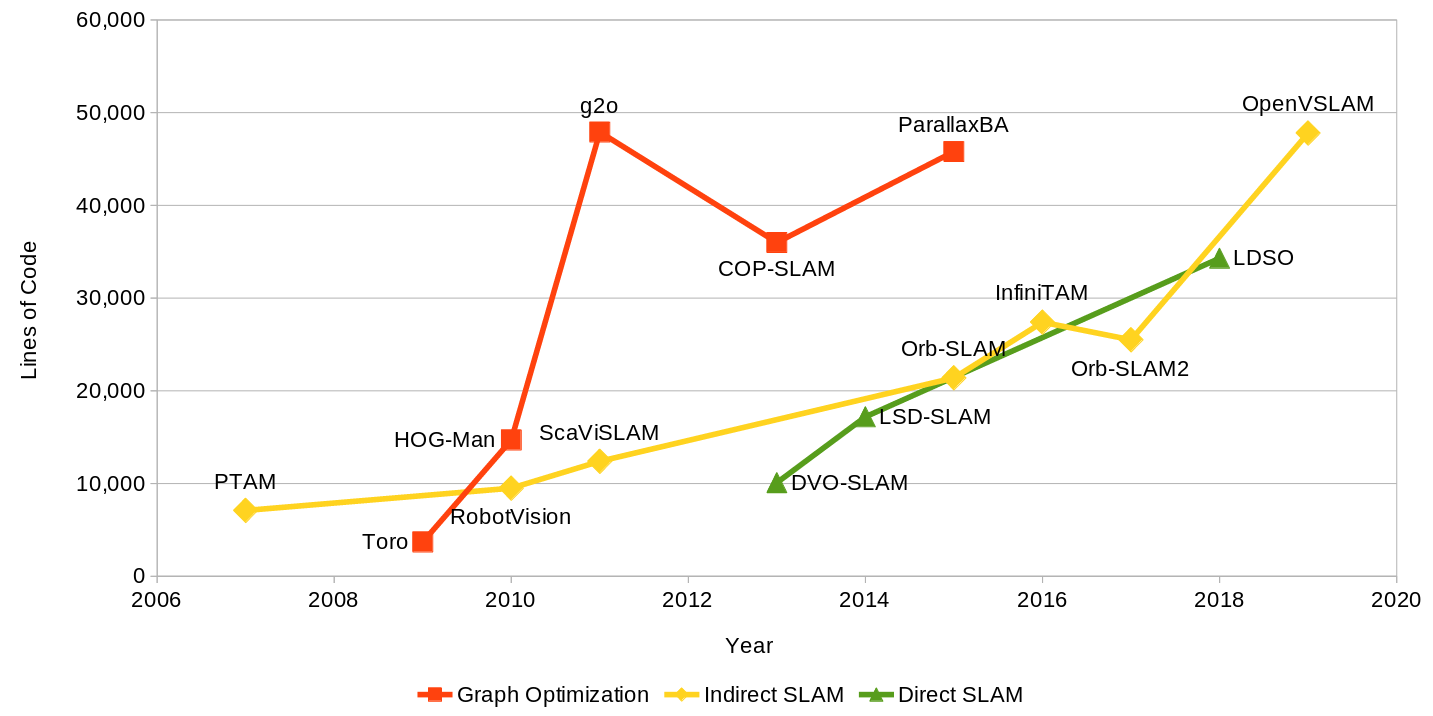
\includegraphics[width=\linewidth]{assets/img/slam-cloc.png}
	\caption{Growth of SLAM libraries over time.}%
	\label{fig:assets/img/slam-cloc}
\end{figure}

Most of SLAM projects are developed using the C++ programming language for performance reasons.
I will argue however, that by continuing to do so, we are hindering mid and long-term research
in the field.
C++ projects are difficult to build, mainly because of assumptions on requirements,
dependency conflicts and usage of Linux, Mac, Windows or architecture specific libraries.
To mitigate those issues, projects tend to include within the source code all of their dependencies.
From the 461k lines of code in OpenMVG, 390k are coming from the \verb|src/nonFree/|
and \verb|src/third_party/| directories.
Although seemingly matters of engineering, those characteristics actually influence research
by putting a very high barrier to entry for new approaches to be able
to reproduce already available results and compare with them.
One should also note that frozing dependency versions brings security concerns,
since upstream security patches requires manual actions to be replicated.
This is especially true in the context of open-source,
where we have less control over contributions.
Even careful companies like Microsoft suffer from C++ memory safety bugs
for 70\% of their critical security issues~\cite{msrc-safer}.
Research code will eventually reach critical software, such as autonomous vehicles.
With great research comes great responsability!

In the second part of this document, we will focus on visual odometry.
Chapter~\ref{cha:rgbd_vo} introduces the visual odometry problem
and the fundamental geometry tools required to modelize it.
Since we aspire to run those algorithms directly in the browser,
Chapter~\ref{cha:performant_web_applications} reviews past and present technologies
enabling high performance computations on the Web.
In particular, we detail how to target a new standard called WebAssembly from C++ and Rust.
In Chapter~\ref{cha:interactive_vo_on_the_web} we present our open-source visual odometry library,
which features a new points selection algorithm for the camera tracking.
We started it from scratch in the Rust programming language,
which allowed us to easily port it to WebAssembly.
Finally, we showcase an interactive visual odometry Web application,
enabling improvements on the tracking and 3D geometry results thanks to user interactions.
A paper describing the open-source library and the interactive application is intended to be published.


\part{Image Annotation}%
\label{prt:image_annotation}
This part is about image annotation.

\chapter{The Image Annotation Problem}%
\label{cha:the_image_annotation_problem}

\adjustmtc
\minitoc%

In this chapter, we introduce the concept of image annotation, and review the body of work that have been researched in this domain. 

Bur first, what is image annotation? The most simple way to put it would be ton consder it as the process of augmenting an image with information. This information can be of various nature (we review the existing annotation in section ???), and is typically provided by a human operator, also called annotator. 

We could consider photogrammetry as the first historical example of image annotation, long before digital images even existed. The process of measuring distances and lengths of the real world from 2D images requires annotating these distances and lengths in the image space, before inferring the values in 3D. Similarly, early techniques in the old cinema involved manually editing the filmstrip to create special effects, which is a form of annotation.

Digital imaging has progressively brought new needs for image annotation. The first digital image was scanned from a photograph in 1957 by Russell Kirsch, and the first digital camera was built in 1975 by the Kodak engineer Steve Sasson. Commercial models of digital cameras became really available in the 1990s, and from then the volume of digital images produced grew exponentially every year.

In the meantime the computer vision community, which originated from the artificial intelligence one, became more and more interested in machine learning. Machine learning designates a class of algorithms in which a model learns from experience, materialized by data samples. One sub-domain of machine, called supervised machine learning, requires in particular annotated samples, meaning that a label should be assigned to each piece of data and an algorithm is trained to predict this label. Supervised machine learning gained traction in the 1990s during which some applications reached high enough maturity to be exploited commercially. A famous example of this is the digit recognition algorithm from Lecun et al. \cite{blabla} which was used by AT\&T to automatically process cheques in ATMs. A nowadays popular dataset, called MNIST (Mixed National Institute of Standards and Technology) was created for this work; this dataset associates labels (digits, from 0 to 9) to $28\times 28$ pixel images of handwritten figures. 

This dataset illustrates how image annotation could be used to produce desirable applications, and is only a small example of what has now become a classic pipeline to solve problems in the computer vision community. Note that while we focus this chapter on computer vision (because image annotation has become key in this community), the machine learning pipeline we introduce is also used in many other problems such as audio processing or natural language processing. 

Theoretical results in machine learning postulate that problems of great complexity could be adressed with this technique, provided that (i) there exists a model of sufficient capacity to cope with the problem complexity, and (ii) a sufficiently large sample of annotated data is available. Some thresholds have been established by the community to estimate what "sufficiently large" means \cite{blabla}, but computer vision problems typically requires millions of (annotated) images to be solved with an acceptable performance. Models relying on deep neural networks are nowadays the most popular techniques in machine learning, but other models (such as deep random forests for example, used in the human body pose estimation embedded in the Kinect \cite{blabla}) may still be considered depending on the application. Note that an important field of today's research now focus on learning on few samples; this field regroups the notions of semi-supervised learning, weakly-supervised learning, one-shot and few-shots learning, etc. 

 




Different types of problem that require annotation:
\begin{itemize}
	\item Image classification: scene (inside/outside : beach, mountain, forest, etc.) and main represented object (see MS COCO)
	\item Image captioning: describe an image with a set of sentences
	\item Object detection and localization : object class + bounding box
	\item Object segmentation : object pixel mask
	\item Image Segmentation. Semantic Segmentation / Image Parsing : classify all pixels in an image
	\item Human Pose annotation, shapes segmentation and similarity, etc.
\end{itemize}
All these annotations have been extended to video \\ \\

What applications to these problems? \\ \\

Different types of interactions for these annotations:

\begin{itemize}
	\item Free text typing
	\item Icon clicking
	\item points, lines
	\item bounding box
	\item polygon
	\item crcles, ellipses ??
\end{itemize}

Other important points:

\begin{itemize}
	\item implicit/explicit annotations
	\item Quality check of the annotations? Self-correcion system? Detection of bad annotations?
	\item expert or non-expert annotation ? Crowdsourcing ?
	\item QoE of the interaction staken into account?
\end{itemize}

THE BIG TABLE: datasets and relevant papers, to be classified



\chapter{Contribution on Outlining}%
\label{cha:contribution_outlining}

Interactive segmentation consists in building a pixel-wise partition
of an image, into foreground and background regions,
with the help of user inputs.
Most state-of-the-art algorithms use scribble-based interactions
to build foreground and background models,
and very few of these work focus on the usability of
the scribbling interaction.
In this paper we study the outlining interaction,
which is very intuitive to non-expert users on touch devices.
We present an algorithm, built upon the existing GrabCut algorithm,
which infers both  foreground and background models out of a single outline.
We conducted a user study on 20 participants
to demonstrate the usability of this interaction,
and its performance for the task of interactive segmentation.


\section{Introduction}


The number of pictures that are captured,
stored and shared online is growing everyday.
In march 2017, Facebook reported that 300 millions pictures
are uploaded each day on their website.
These pictures are increasingly used by companies,
or even by individual users, enabling new applications
trying to improve everyday life.
Object segmentation constitutes an important step
towards automatic image understanding which is key
to those smart applications.


Object segmentation in an image remains a challenging task.
This process of assigning a label to each pixel is very sensitive
to the classical difficulties encountered in computer vision:
lightning conditions, occlusions, etc.
Recent advances in deep learning have enabled researchers to obtain
state-of-the-art results~\cite{long2015fully} by training
on the PASCAL segmentation dataset~\cite{everingham2010pascal}.
Some other techniques learn to infer a pixel-wise segmentation
out of weak annotations, i.e.\ bounding boxes around
objects~\cite{papandreou2015weakly}.
These methods are very promising but need huge amount of human labeled
samples in order to train the deep neural network.
Recent approaches have tried to overcome this issue,
introducing active learning to train deep neural networks
using a limited amount of selected samples~\cite{liu2017active},
on the problem of image classification, but none of these methods
have yet been applied on semantic segmentation.


Because automatic segmentation is still in many cases
out of algorithms' reach, researchers have introduced
the concept of interactive segmentation.
This problem has often been approached with a task-driven point of view:
what type of interaction may bring the necessary information
to significantly help an algorithm achieve an acceptable segmentation?


\begin{figure}[hb]
\centering
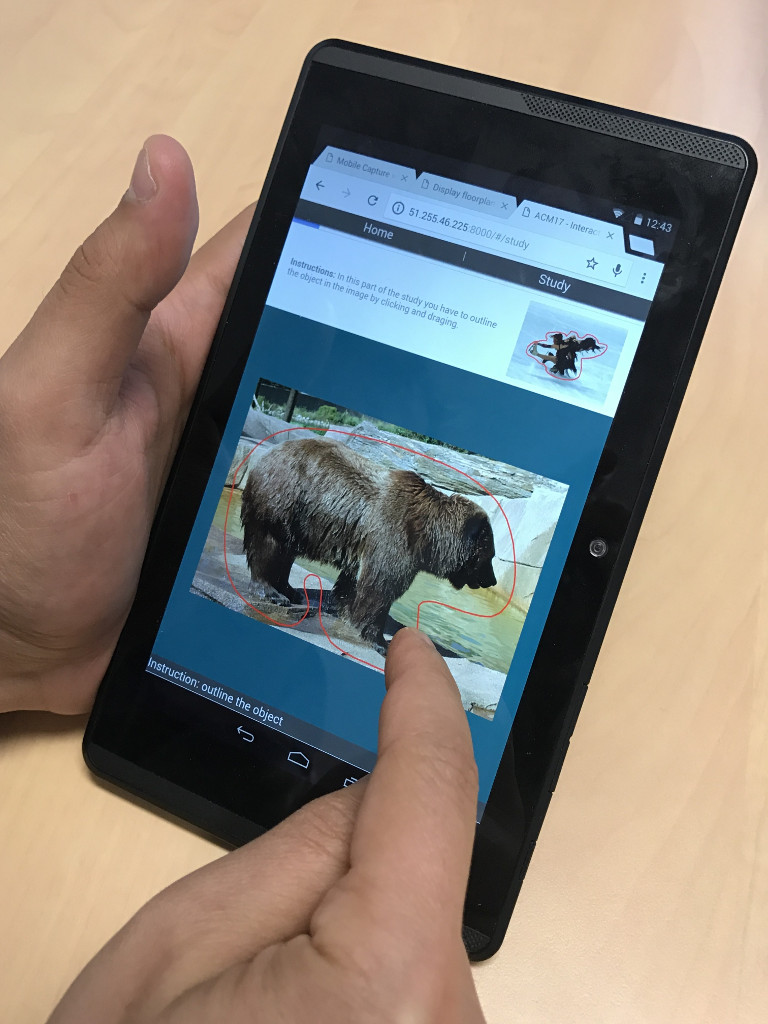
\includegraphics[width=0.4\columnwidth]{assets/img/photo_tablet.jpg}
\hfill

\includegraphics[width=0.55\columnwidth]{assets/img/bear_02_mask.png}
\caption{A user outlining an object on a touch device,
and the resulting segmentation mask obtained with our method.}%
\label{fig:bigpicture}
\end{figure}


The users providing the interactions are always supposed
to have a fair understanding of what segmentation is.
This assumption is problematic, especially when putting
into perspective the extraordinary amount of images to be annotated.
That is why, in this paper, our target population is composed
of non-expert users who are not knowledgeable
about image processing and segmentation.
As a consequence most of the existing work, which rely on foreground
and background scribbles and require a high cognitive load
from the users, are not suitable to our problem.


Instead, we propose to use an intuitive interaction,
outlining (see Figure~\ref{fig:bigpicture}),
that can be performed quickly and lead to good segmentation results
while keeping users from entering a process
of iterative segmentation refinement.
This outlining interaction is particularly well suited
for touch devices, which is appropriate considering the growing
usage of tablets and smartphones compared to computers.
All these properties make the outlining interaction very interesting
for crowdsourcing segmentation annotations on thousands of images,
with non-expert users.


We present two main contributions in this work:
first, a modification of the GrabCut algorithm
that takes as input an outlining interaction, instead of a bounding box.
We take advantage of the free-form shape drawn by the users
to extract information about foreground
(using the Blum Medial Axis computation)
out of a background annotation (the outline).
The second contribution of this work is the usability comparison
of various interactions that are used in interactive segmentation.
We argue that the outline offers the advantage of being a quick,
easy-to-understand and usable interaction while providing
a high amount of supervision to obtain a good segmentation.


The rest of the paper is organized as follows:
we first review the related work in Section~\ref{sec:soa},
we then explain our method to compute segmentation masks
out of outlining interactions in Section~\ref{sec:method}.
Finally we present our experiments and the results we find
that prove our simple interaction can lead to
a good quality segmentation in Section~\ref{sec:experiment}.


\section{Related Work}%
\label{sec:soa}


\subsection{Existing interactions for user-assisted segmentation}


Many interactions have been explored in the literature
to provide users with a way to bring semantic information
to help a segmentation algorithm.
We review the interactions in this paragraph
and present briefly the algorithms that are attached to them.


The most intuitive methods are the ones that require
the user to manually designate the contours of the object.
The LabelMe tool~\cite{russell2008labelme}
(see Figure~\ref{fig:labelme}) is the most famous example
of such an interface.
The web-based interface developed by the authors
allows users to draw a polygon around an object.
The segmentation obtained with this technique
is not necessarily precise at the pixel level,
but is sufficient in many cases and has the advantage of being easy
for users.
In a variant of this technique called
the Intelligent Scissors~\cite{mortensen1995intelligent},
the users click points on the contour of the object and a dynamic
programming algorithm searches the optimal path that ties those points.
There exists another variation of contour drawing called
Soft Scissors~\cite{wang2007soft}.
One has to follow the contour using a soft constrained,
size-adaptable thick contour brush,
requiring less precision than exact polygon contour drawing.


\begin{figure}[ht]
\centering
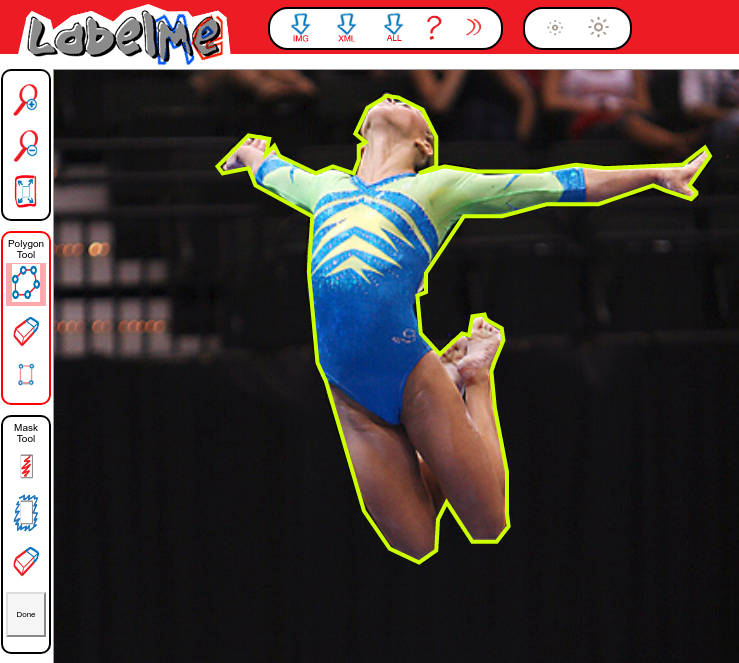
\includegraphics[width=0.8\columnwidth]{assets/img/LabelMe.jpg}
\caption{Visualization of an image annotated with the LabelMe tool~\cite{russell2008labelme}}%
\label{fig:labelme}
\end{figure}


A second possibility for interactive segmentation has been proposed
by Rother et al.~\cite{rother_grabcut:_2004}.
The user is only required to draw a bounding box around the object
(see Figure~\ref{fig:rect_scrib}), which is used to learn
a background model. The foreground is then obtained
using iterative graph-cut and alpha matting.
This method  works very well for object that distinctly emerge
from a repetitive background.
However in the case of complex scenes, the authors allow users
to perform an additional refining step based on scribbles.


\begin{figure}[ht]
\centering
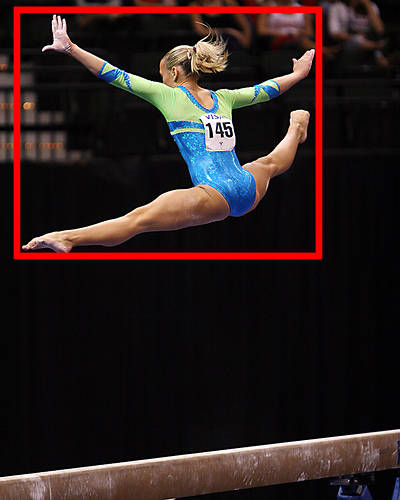
\includegraphics[width=0.45\columnwidth]{assets/img/gymnast_rect.jpg}
\hfill
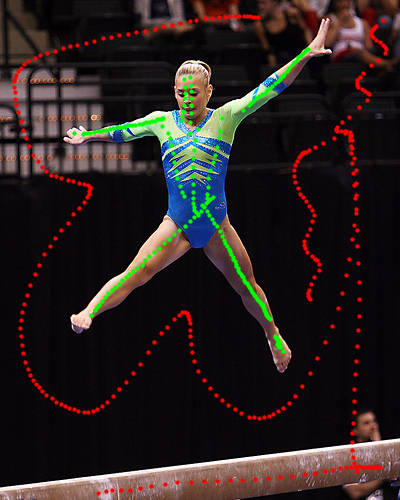
\includegraphics[width=0.45\columnwidth]{assets/img/gymnast_scrib.jpg}
\caption{Example bounding box and scribbles interactions.
In the left image, a user drew a bounding box around the gymnast.
In the right image, a user drew green foreground scribbles
on the gymnast and red background scribbles outside.}%
\label{fig:rect_scrib}
\end{figure}


Scribbles form another category of interactions for segmentation,
and are undoubtedly the most widely used
(see Figure~\ref{fig:rect_scrib}).
Users can typically draw foreground and background scribbles
on the image, and receive a feedback on the current state
of the resulting segmentation mask.
Boykov and Jolly~\cite{boykov_interactive_2001} use this input to build a trimap,
i.e.\ a partition of the image into  hardly constrained foreground
and background regions, and a softly constrained in-between region.
They run a graph-cut algorithm to find the optimal object boundary
on the softly constrained region.
McGuinness and O’Connor~\cite{mcguinness2010comparative} describe
how to use scribbles to segment an image using
a Binary Partition Tree (BPT)~\cite{salembier2000binary}.
The BPT is a hierarchy of image segments that can be used to propagate
the foreground and background inputs between similar regions.
Scribbles have also been used in the context of
image co-segmentation~\cite{batra_icoseg:_2010},
to provide foreground and background information across
a set of images depicting the same object.
As an alternative to scribbles, single foreground and background points
have been used as input to select the best masks
among a set of object candidates~\cite{carlier_clickncut:_2014}.


The mouse is used in most of these work as interaction device,
which probably explains why outlines are rarely studied in the literature.
Outlines are indeed tedious to perform with a mouse.
However, most of the literature algorithms can take outlines as an input;
in our work we choose to use GrabCut to obtain
a segmentation out of the outlines.


\subsection{Interactive segmentation for non-expert users}


Although many work have studied how to incorporate human interactions
into segmentation algorithms, there are only very few authors
who studied interactive segmentation with a special focus
on the interaction matter.
In particular, the distinction between experts and non-expert users
has rarely been made when studying
the performance of interactive segmentation algorithms.
Considering the tremendous number of ground truth masks needed
to train deep learning algorithms to segment images,
the human annotations necessarily have to be provided by non-expert users.
Some experiments on crowdsourced
segmentation~\cite{carlier2016assessment} clearly show that
non-expert users can misunderstand a simple
segmentation HIT (Human Intelligence Task),
mistake foreground and background colors,
misunderstand the segmentation feedback, etc.


As a matter of fact, most of the crowdsourcing efforts in interactive
segmentation have been performed with a LabelMe type of interface.
In addition to the actual LabelMe project,
some work on medical imaging have crowdsourced segmentation masks by
asking users to draw a polygon around
hip joints~\cite{chavez2013crowdsourcing},
muscle and melanoma cells~\cite{gurari2015collect},
and nuclei~\cite{irshad2014crowdsourcing}.


However, those work do not specifically aim at
the usability of their interfaces. Recent works by
Korinke et al.~\cite{korinke_intuitive_2015,korinke_exploring_2015}
give insights on the preferred user interactions
for interactive image segmentation on mobile devices.
Dividing the process into two steps, initialization and refinement,
seems to be the preferred input method.
The initial step can be either bounding box drawing or a simple outline.


Our work is largely inspired by these findings;
since we target non-expert users, we want to provide
the most natural interaction and choose outlining
for our interactive segmentation algorithm.


\section{Outlining objects for interactive segmentation}%
\label{sec:method}


In this section we explain why we use outlining annotations,
and our method to compute segmentation masks out
of outlining interactions.


As stated in the previous section, most of prior crowdsourcing
campaigns in image segmentation have asked users to draw
a polygon around the object.
This interaction has some merit in terms of usability:
it is very straightforward to understand,
and does not require iterative refinement from the user.
In addition, the user does not have to evaluate the quality
of the produced segmentation mask to know when to stop interacting.
When the polygon is drawn, the segmentation is over.


However, we have two main concerns with this interaction.
First, it is tedious and time consuming. It requires  users' full
attention, in order to precisely click on the object boundary.
It also requires users to implicitly determine the number
of edges of the polygon they should draw.
A second limitation of this interaction is the quality
of the segmentation mask obtained.
Shape details and curved boundaries can only be approximated by a polygon,
and their quality is correlated with the time
the human annotator is willing to spend annotating.


Outlining an object has the same merits than drawing a polygonal shape
around the object: the task is easily defined,
and it is easy for a user to assess the quality of an outline.
It also adresses the first limitation of the polygons:
since it requires less precision in following the object boundaries,
it is less tedious and time consuming.
It has nevertheless an important drawback:
it does not provide an accurate segmentation.


In order to address this problem, we choose to rely on the popular
Grabcut algorithm~\cite{rother_grabcut:_2004}.
The original GrabCut takes a bounding box as an input.
It considers every pixel outside of the bounding box as fixed background,
and aims at separating foreground from background inside the bounding box.
To this end, a background model is estimated from the fixed background,
and a foreground model is estimated from the pixels
inside the bounding box.
The likelihood of each pixel inside the bounding box
to be foreground or background is then estimated,
and graph-cut is applied to obtain a temporary segmentation mask.
This mask is then used to update the foreground and background models,
and the process is iterated until convergence.


In our implementation, we slightly alter the GrabCut algorithm to take
into account a major difference between outlines and bounding boxes:
we can make stronger assumptions on the foreground positions
from an outline than from a bounding box,
by looking at the general shape of the outline.
We restrict the initial foreground model computation to the pixels
that are most likely to be foreground,
which decreases the number of iterations needed for convergence
and improves the segmentation quality.


In the rest of the section, we explain two different methods
to infer foreground out of the ouline shape:
the first method consists in eroding the outline,
and the second is based on the Blum medial axis computation.
We then post-process the foreground pixels using superpixels.


\begin{figure}[ht]
\begin{subfigure}[b]{0.49\columnwidth}
    
\includegraphics[width=\textwidth]{assets/img/outlineEroded.png}
    \caption{Erosion of outline}%
    \label{fig:outlineEroded}
\end{subfigure}
\hfill
\begin{subfigure}[b]{0.49\columnwidth}
    
\includegraphics[width=\textwidth]{assets/img/outlineSkel.png}
    \caption{Skeleton of outline}%
    \label{fig:outlineSkel}
\end{subfigure}
\begin{subfigure}[b]{0.49\columnwidth}
    
\includegraphics[width=\textwidth]{assets/img/outlineErodedSP.png}
    \caption{Erosion of outline extended with superpixels}%
    \label{fig:outlineErodedSP}
\end{subfigure}
\hfill
\begin{subfigure}[b]{0.49\columnwidth}
    
\includegraphics[width=\textwidth]{assets/img/outlineSkelSP.png}
    \caption{Skeleton of outline extended with superpixels}%
    \label{fig:outlineSkelSP}
\end{subfigure}
\caption{Different foreground inferring methods from a user outline.
The ground truth mask is in dark blue.
The user outline is in cyan.
The inferred foreground is in yellow.}%
\label{fig:foreground}
\end{figure}


\subsection{Outline erosion}%
\label{sec:erosion}


The simplest method to obtain points that are likely to be foreground
from an outline is to apply morphological erosion
of a mask representing the inside points of the outline.
We use a disk as a structuring element for the erosion,
and the only parameter of this method is the radius of the disk.


In our implementation, the disk radius is specific to each user
and computed by studying the outline performed by the user
on a Gold Standard image.
We compute the mean $m_d$ and standard deviation $s_d$ of
the distance $d$ from each outline point to the ground truth mask.
Assuming the user consistently outlines all images,
i.e.\ the mean distance of the user outline to an object
is more or less constant across all images,
a disk radius equal to $m_d + 2 \cdot s_d$ should produce an
eroded outline that is almost certainly completely foreground.


An example of this process can be visualized
on Figure~\ref{fig:outlineEroded}.
The eroded outline (yellow) is almost entirely contained
in the ground truth mask (dark blue).


\subsection{Blum medial axis algorithm}


In shape analysis and model animation, the Blum medial axis
transform~\cite{blum1978shape} is one of the most popular tools.
The Blum medial axis of a shape is composed of the centers
of the circles that are tangent to the shape in at least two points.
It is especially appropriate to compute skeletons,
composed of the medial axis points inside the shape.


\begin{figure}[ht]
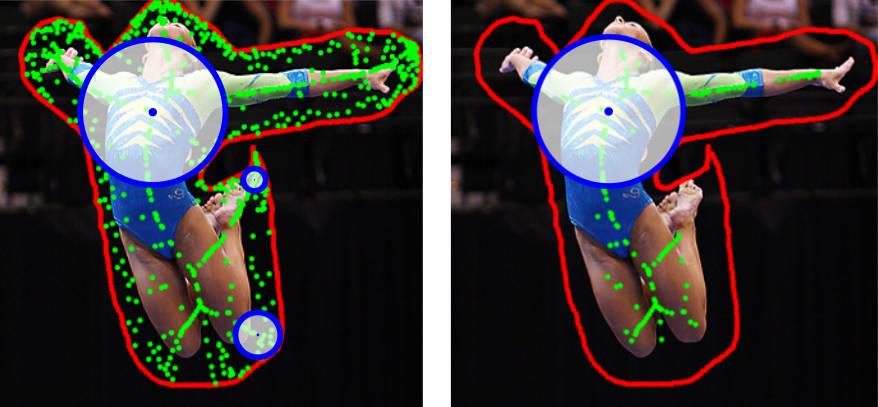
\includegraphics[width=\columnwidth]{assets/img/skeleton.jpg}
\caption{Skeleton (in green) computed using the Blum medial
axis algorithm from an outline (in red).
Few example disks are shown in blue.
In the image on the left, all disks centers (green points) are kept,
generating a very noisy skeleton.
In the image on the right the skeleton is pruned,
by filtering out centers of small disks.}%
\label{fig:skeleton}
\end{figure}


One of the problems of the medial axis algorithm is its stability
when the shape frontier is noisy.
It tends to create a high number of branches
(see Figure~\ref{fig:skeleton}),
which deteriorates the simplicity of the skeleton,
and incidentally the comprehension of the shape.
In our case, this is rather an advantage.
Indeed more ramifications lead to a higher number of points
inside the shape for our foreground scribbles.
However, we need to filter the inside points,
since those close to the outline have a high probability
of being outside of the object to segment.
Radius of the inside circles of medial axis points
constitute a good filter option,
because the medial axis points with the smaller radius are typically
close to the outline and appear as a consequence of the outline noise.
In our implementation, we choose to keep only centers
with a radius higher than half the larger radius.
Figure~\ref{fig:outlineSkel} depicts a ground truth mask in dark blue,
a user outline in cyan and the filtered medial axis points in yellow.
Most of the yellow points fall inside the ground truth mask,
thus making it a good starting point to learn the foreground model.


\subsection{Enhancing foreground with superpixels}%
\label{sec:superpixels}


These two methods, Blum medial axis and outline erosion,
allow to select foreground points that make a valuable input
to the GrabCut algorithm.
However, we add a post-processing step to (i) extend this foreground
information and (ii) filter as much false foreground points as possible.


To do so, we compute a superpixels segmentation of the image,
i.e.\ an oversegmentation that groups neighbouring pixels
with similar colorimetric properties.
We (i) extend the foreground labels from pixels
to the superpixels they belong to.
This considerably increases the surface of the foreground region.
In addition, we (ii) handle conflicting superpixels,
which contain both pixels denoted as foreground and a piece of the outline,
by removing them from the foreground mask. An example of the result
can be seen on Figure~\ref{fig:outlineErodedSP}
and Figure~\ref{fig:outlineSkelSP}.
Note that the errors arising from the first step
(between the knees in Figure~\ref{fig:outlineEroded}
and Figure~\ref{fig:outlineSkel})
have successfully been removed
in the post-processed inferred foreground mask.


We choose to use the Mean-Shift superpixels~\cite{comaniciu2002mean}
because no compacity constraint is used in their computation.
As a consequence, a superpixel can cover a large area
(especially in the case of similar background regions,
such as an homogeneous sky) and will more likely correct
wrongly inferred foreground points.


%%%%%%%%%%%%%%%%%%%%%%%%%%%%%%%%%%%%%%%%%%%%%%%%%%%%%%%%%%%%%%%%%%%%%%%


\section{Experiments}%
\label{sec:experiment}


In this section we describe the setup of our experiments
and analyze the outcome of the study.


\subsection{Experimental setup}


\textbf{Interactions}
Since the purpose of the study is interactive segmentation on touch devices,
we choose to compare only three annotations:
outlines, scribbles, and bounding boxes.
We do not include polygon drawing because
it is clearly not adapted to a touch device.
Indeed, fingers are too big to precisely touch the boundary of an object,
they would hide the area where the user would try to place the vertex on.


The interfaces are kept as simple as possible.
The user is shown an image and has to provide a valid input
to be allowed to move on to the next image.


\begin{figure}[ht]
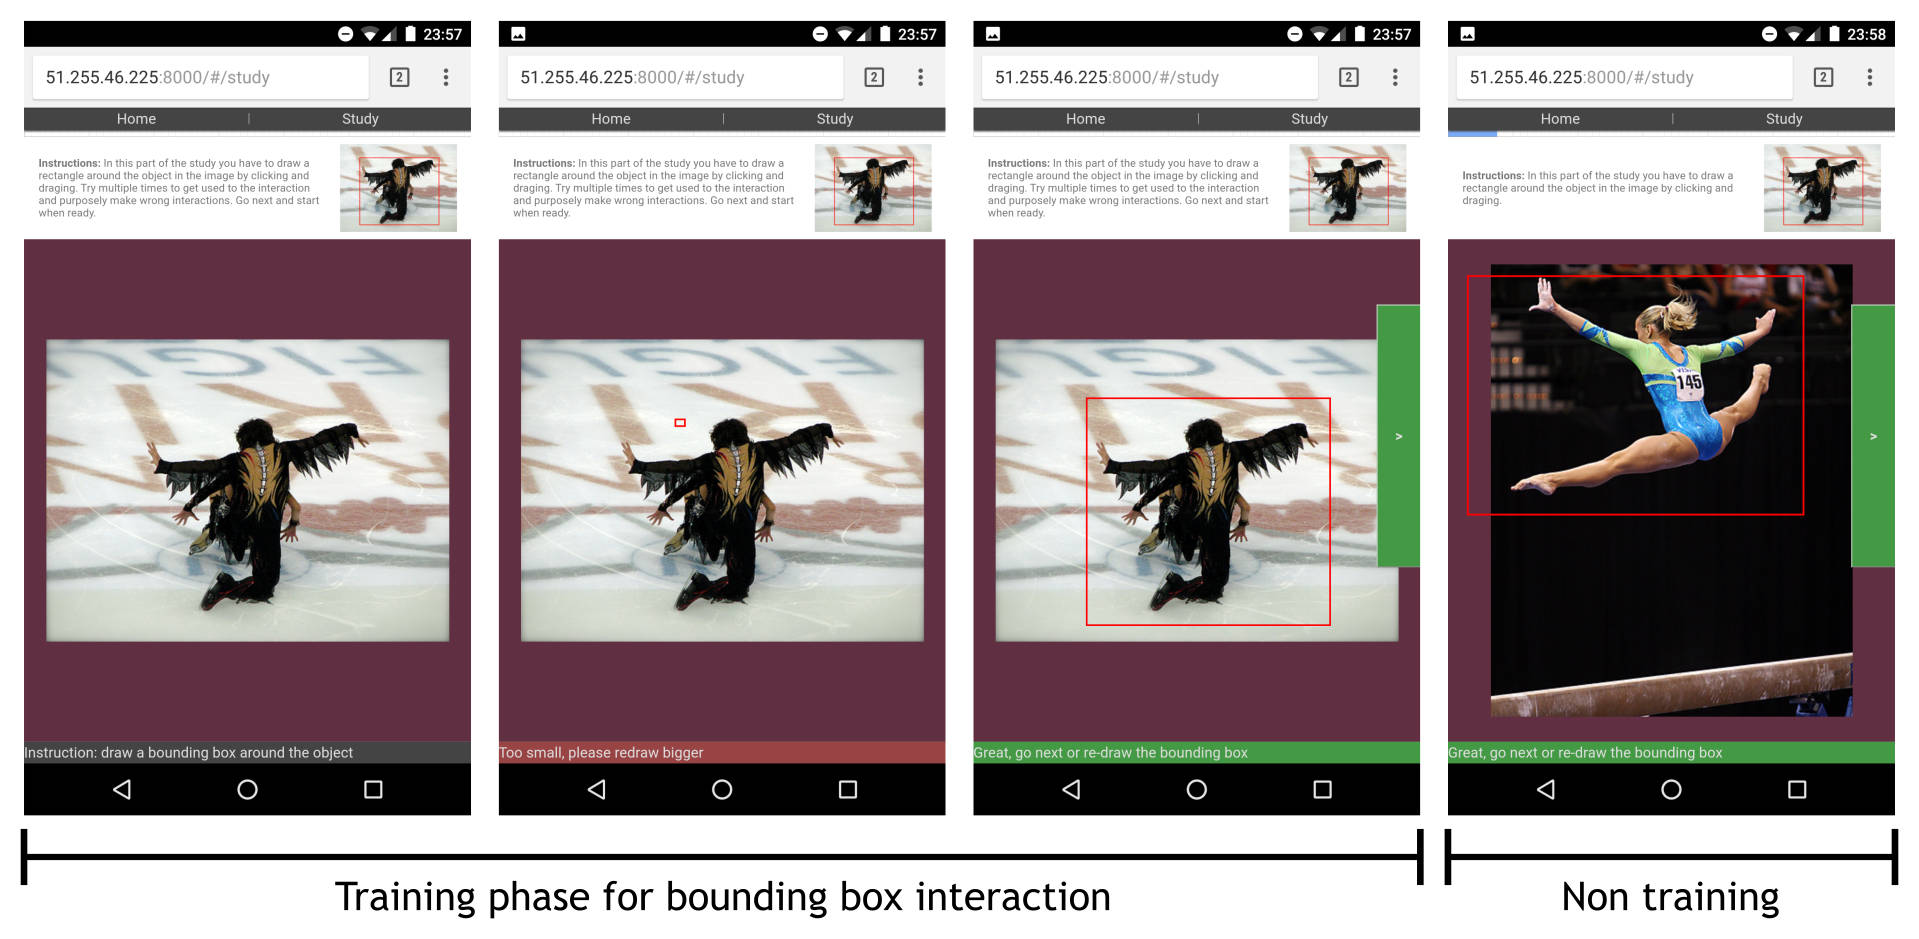
\includegraphics[width=\columnwidth]{assets/img/app_rect.jpg}
\caption{Several screenshots of the bounding box interface
during training phase (left), and during the study (right).}%
\label{fig:rectangle}
\end{figure}


The bounding box interface allows the user to draw a rectangle
over the image using a touch and drag interaction.
If the user is not satisfied with their previous attempt,
they can start over, which will replace the former rectangle with a new one.
The user can only move on to the next image when the current rectangle
is of sufficient size (we discard rectangles
that are too small to avoid common mistouch issues).


\begin{figure}[ht]
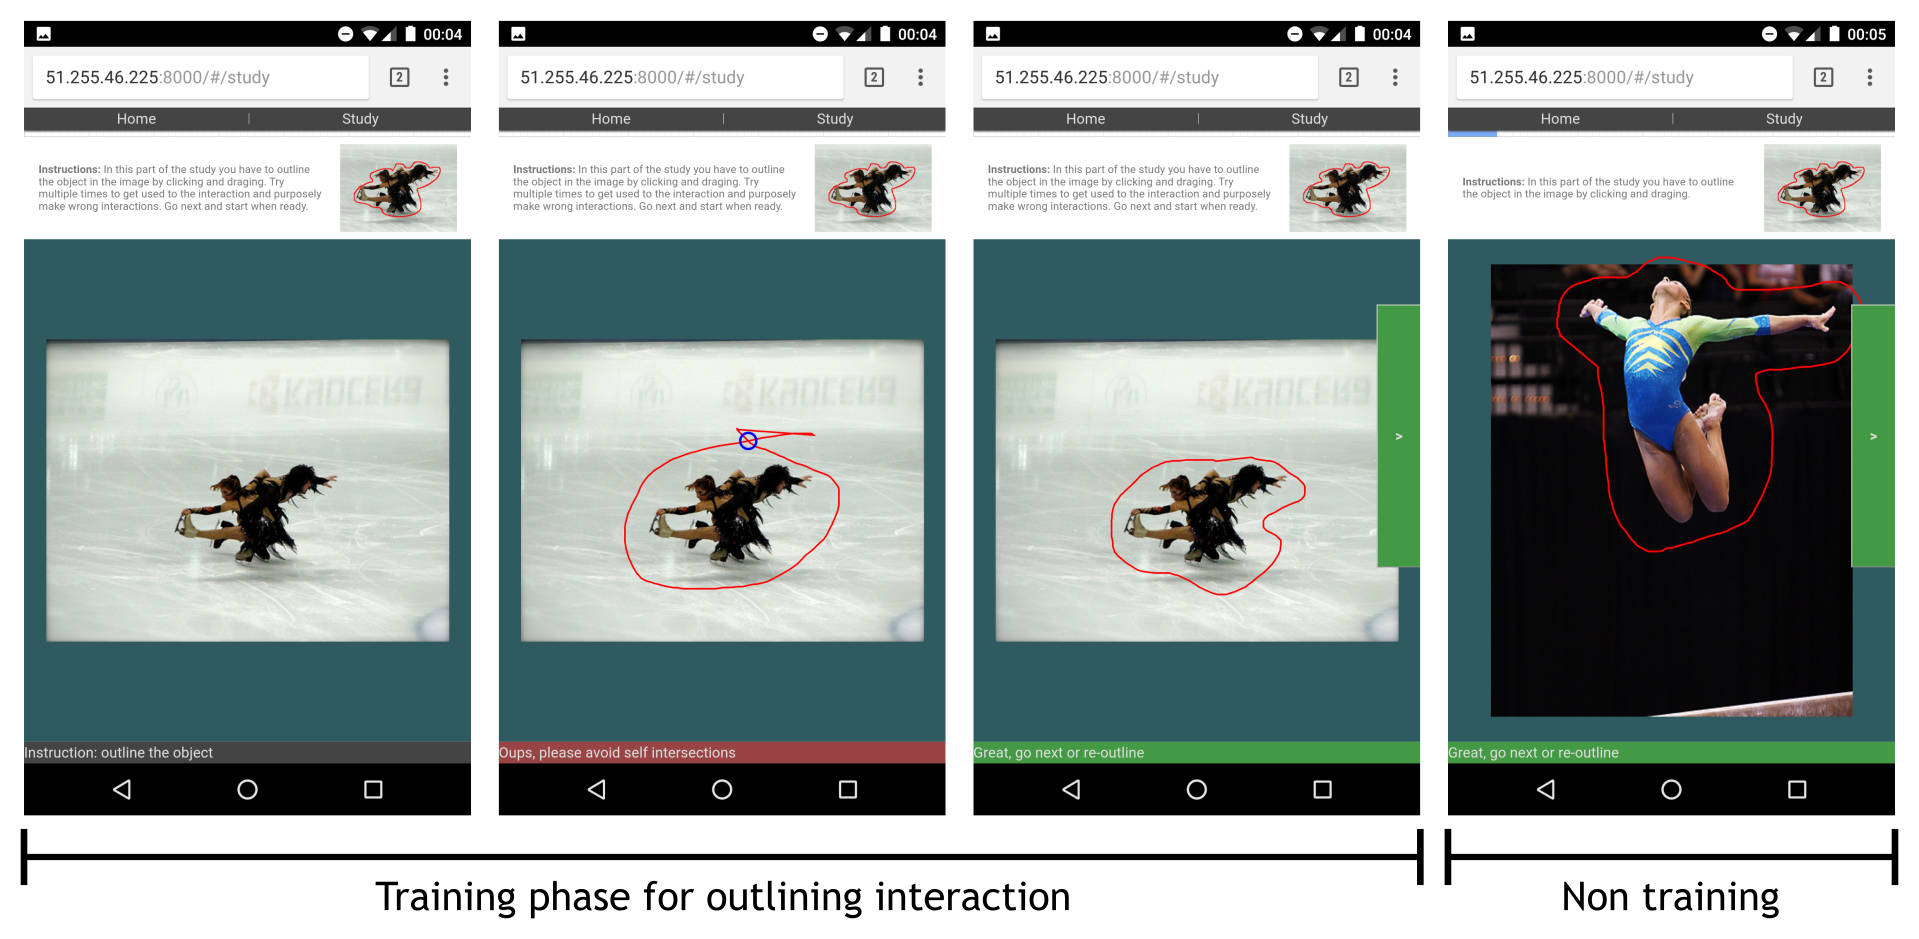
\includegraphics[width=\columnwidth]{assets/img/app_outline.jpg}
\caption{Several screenshots of the outlining interface
during training phase (left), and during the study (right).}%
\label{fig:outline}
\end{figure}


The outlining interface is very similar to the bounding box interface.
The user can draw the outline using a touch and drag interaction;
the system automatically draws the closing segment between
the ending and starting points when the user releases their finger.
The user can also start over if not satisfied with the current outline.
The system allows the user to move on to the next image
if the outline is of sufficient area.
In addition, for the training image only,
the system checks the absence of loops in the outline path
(see Figure~\ref{fig:outline}), for they may reveal incorrect usage.
This loop detection feature is deactivated for the other images
to limit its impact on the interaction and user frustration.


\begin{figure}[ht]
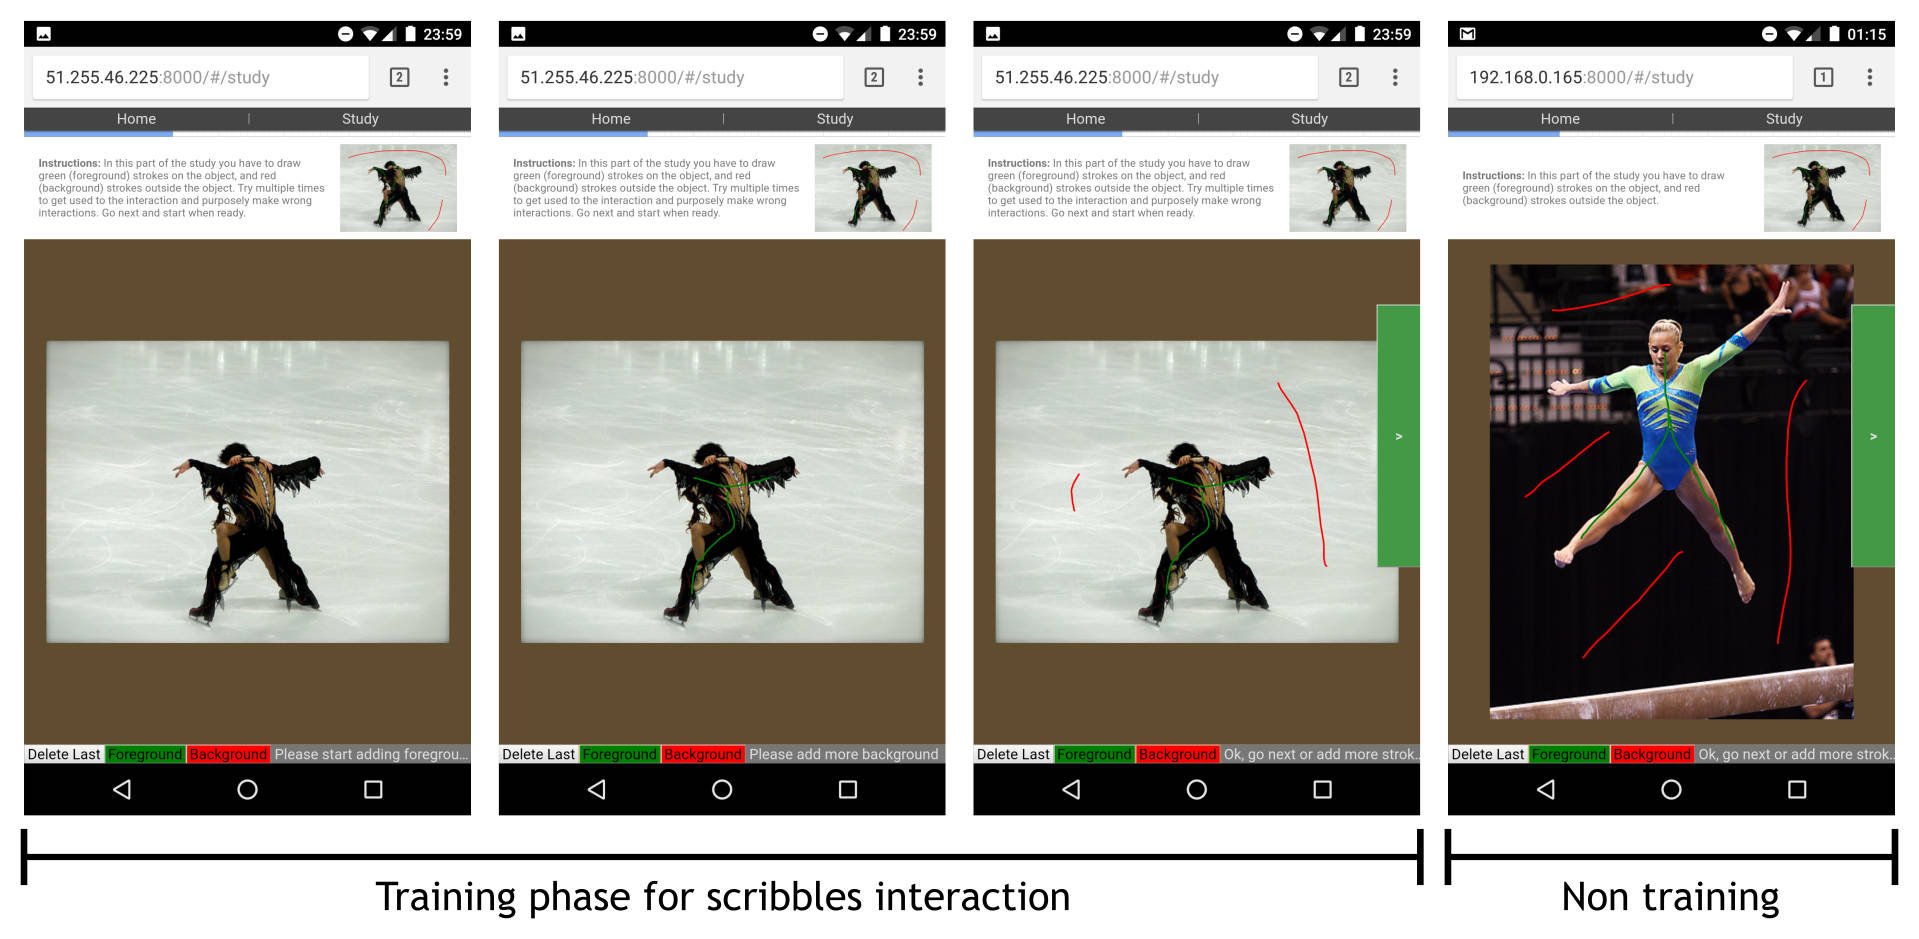
\includegraphics[width=\columnwidth]{assets/img/app_scribbles.jpg}
\caption{Several screenshots of the scribbling interface
during training phase (left), and during the study (right).}%
\label{fig:scribbles}
\end{figure}


The scribbling interface displays three buttons:
one to select the foreground scribbles, which are drawn in green,
one to select the background scribbles, which are drawn in red,
and one to remove the last drawn scribble.
Users are required to provide a certain scribble length
to be allowed to move on to the next image.


\textbf{Device and software}
We used a regular 8'' android tablet,
for which the buttons appeared large enough to be easily clickable.
The user study being a web application,
it was conducted in the chrome browser for android.
The code for this study (web client and server),
as well as the results presented here are all available online
(github.com/mpizenberg/otis).


\textbf{Images}
We select 36 images from the iCoseg dataset~\cite{batra_icoseg:_2010},
which we divide into 3 groups of 12 images.
We want the segmentation results to be comparable between
different interactions, but since each user tests the three interfaces,
we do not want to use the same images for the three phases of the study.
This would indeed risk biasing the results:
users might get annoyed of annotating three times the same images
and this could affect the quality of their annotation, for example.


The iCoseg dataset provides multiple images depicting the same object
in different situations.
Examples of these images can be seen on Figure~\ref{fig:icoseg}.


\begin{figure}[ht]
\centering
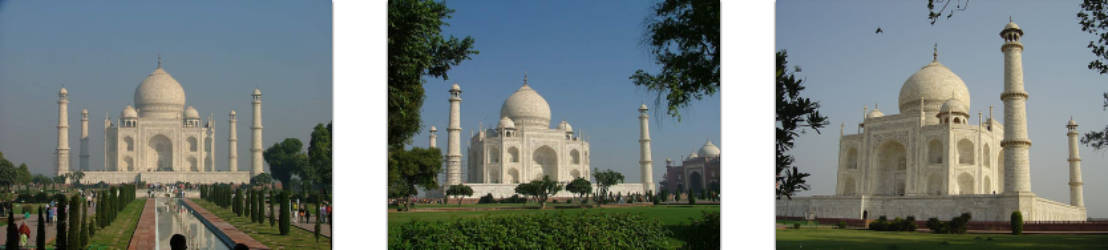
\includegraphics[width=\columnwidth]{assets/img/taj_mahal.jpg}
\vfill\vspace{0.5em}\vfill
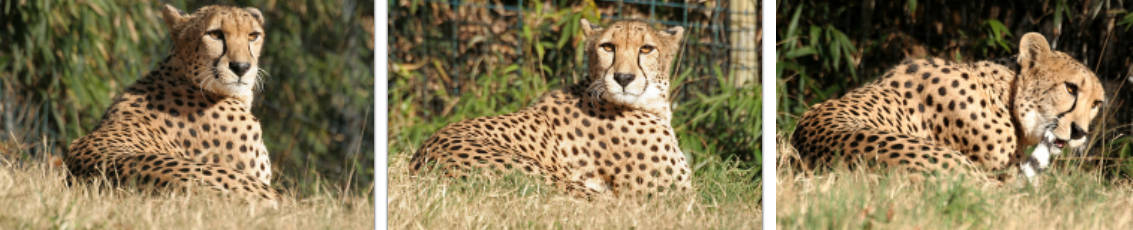
\includegraphics[width=\columnwidth]{assets/img/cheetah.jpg}
\caption{Some images from the iCoseg dataset}%
\label{fig:icoseg}
\end{figure}


\textbf{Methodology}
The protocol of the study is as follows.


The users are not explained the concept of segmentation,
we tell them that we require annotations on images,
and that we wish to compare three interactions to provide those annotations.


The study is composed of three steps, one step per interaction.
For each step, the evaluator first explains the user how
the interaction works, and demonstrates it on a training image.
The evaluator demonstrates good and bad examples of interactions.
Then the user tests the interaction on the same training image.
The evaluator can correct the user and criticize or validate
the users interactions.
Once the user completely understands the tool,
the eleven other images are proposed for interaction.
Finally, at the end of each step,
the user answers two questions about the interaction.


In order to limit bias, the order of the interactions is randomized,
as well as the order of appearance of each image during each step.


Among the eleven images annotated by the user,
one is considered Gold Standard.
It is introduced to (i) check whether the user is performing the task
correctly (this is particularly useful in a crowdsourcing context),
and (ii) to learn the radius of the erosion disk
(see Section~\ref{sec:erosion}).


The two questions asked at the end of each step of the study are:
\begin{itemize}
\item Overall, I am satisfied with the ease of
 completing the tasks in this scenario
\item Overall, I am satisfied with the amount of time
 it took to complete the tasks in this scenario
\end{itemize}
The users can answer on a scale
from 1 (strongly agree) to 7 (strongly disagree).
We choose to ask only these two questions because we are not trying
to assess the usability of a whole system, but only of an interaction.
A standard usability questionnaire,
such as SUS (used in~\cite{korinke_exploring_2015}),
was not really adapted to our use case and instead
we extracted these two questions from a popular post-task questionnaire
(ASQ, After Scenario Questionnaire).


Finally at the end of the study, we ask users to rank
the three interactions in their order of preference.


\textbf{Participants}
Twenty users (10 Male, 10 Female) participated to this study,
with ages ranging from 25 to 55 years old.
Most users have no experience in image segmentation,
and some of them are familiar with the concept.


\subsection{Usability metrics}


Among the criteria stated by Nielsen~\cite{nielsen1994usability}
as defining the usability of a system,
we are able to evaluate efficiency, errors, and user satisfaction.


Efficiency designates the swiftness with which users were able
to complete the tasks once they learned how to interact with the system.
We evaluated this criteria both subjectively,
by asking users about their perception of the time
they spent on the task (table~\ref{tab:questionnaire}),
and objectively by measuring the time it took them to complete their
interactions on each image (see Figure~\ref{fig:timeinteraction}).


User satisfaction is measured through our questionnaire,
both by the question on the perceived task easiness
and the interaction ranking.


Finally, errors are measured by counting the number of times
the users redrew a bounding box or an outline around the object
(for the bounding box and outline interactions),
and by the number of clicks on the \textit{Undo last scribble} button
in the case of the scribbling interaction
(see Figure~\ref{fig:errorinteraction}).


\begin{table}[ht]
\begin{tabular}{lrrr} \toprule
Method & Bounding box & Outline & Scribble \\ \midrule
Ease & 2.1 $\pm$ 0.62 & 2.65 $\pm$ 0.74 & 2.1 $\pm$ 0.61 \\
Time & 2.35 $\pm$ 0.69 & 2.5 $\pm$ 0.67 & 2.6 $\pm$ 0.70 \\
Rank & 1.95 $\pm$ 0.43 & 1.90 $\pm$ 0.32 & 2.15 $\pm$ 0.37 \\ \bottomrule
\end{tabular}
\caption{Results of the questionnaire with a 95\% confidence interval}%
\label{tab:questionnaire}
\end{table}


\begin{figure}[ht]
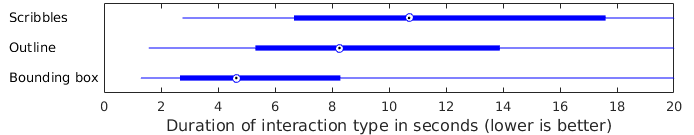
\includegraphics[width=\columnwidth]{assets/plot/interactions_durations.png}
\caption{Duration of interactions, on all images and all users.
The dots are the median durations, and the thick blue line limits
the first and third quartiles.}%
\label{fig:timeinteraction}
\end{figure}


\begin{figure}[ht]
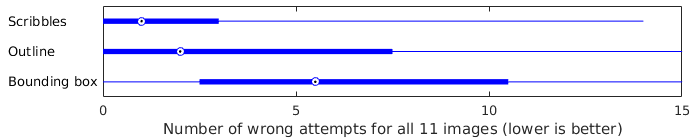
\includegraphics[width=\columnwidth]{assets/plot/interactions_errors_per_user.png}
\caption{Number of errors per interaction and per user on all images.
The dots are the median number of errors,
and the thick blue line limits the first and third quartiles.}%
\label{fig:errorinteraction}
\end{figure}


Overall, the questionnaire results can not allow us to conclude
on the superiority of one interaction method over the others.
Although slightly in favor of the bounding box interaction,
the perceived ease and time are not statistically better
for any of the three interactions.
However the results are all between 2 and 3 (on a scale from 1 to 7),
which mean users were mostly satisfied with all three interactions.
We can note that the time perception results
(table~\ref{tab:questionnaire}) are correlated with the
objective duration of interaction (Figure~\ref{fig:timeinteraction}),
measured during the experiments.
The bounding box is obviously the quickest interaction,
while the scribbles suffer from the time needed to switch between
foreground and background scribbling.


Surprisingly, the outline ranks first in the users preference
(although not significantly), ahead of the bounding box interaction.
The reason of this observation, as explained by many of the participants
during the experiment, is due to to the frustration
that can arise when trying to draw a bounding box
around a non-convex object.
Users who were trying to draw the bounding box as close as possible
from the object boundary often had to use several attempts,
because of the difficulty to position the first bounding box corner.
This problem is very visible on Figure~\ref{fig:errorinteraction},
which shows the high number of errors made by users when
drawing the bounding box.
The errors that occurred during the outline study were mostly due
to a too high interaction speed, or to the users hand masking
the object during interaction,
for users who were the less familiar with touch devices.


\subsection{Interactions informativeness}


We define the background area of user inputs as follows.
For a bounding box (resp.\ outline), the background area is composed
of all pixels outside of the bounding box (resp.\ outline).
For scribbles, the background area is the union of the superpixels
annotated as background (containing part of a background scribble).


\begin{figure}[ht]
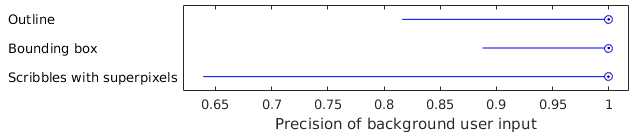
\includegraphics[width=\columnwidth]{assets/plot/precision_bg_all.png}
\caption{Precision of background user input}%
\label{fig:precision_bg}
\end{figure}


\begin{figure}[ht]
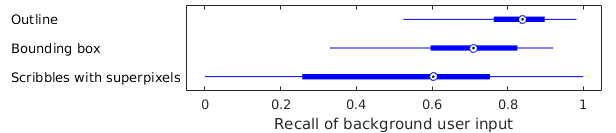
\includegraphics[width=\columnwidth]{assets/plot/recall_bg_all.png}
\caption{Recall of background user input}%
\label{fig:recall_bg}
\end{figure}


Looking at the precision of background user inputs
(Figure~\ref{fig:precision_bg}) we see that more than
75\% of user annotations are perfect (a precision score of 1).
This means that 75\% of user inputs do not intersect at all
the object of interest.
We can conclude that users understand well the tasks they are given.


In order to estimate the informativeness of an interaction,
we also measure the recall index (Figure~\ref{fig:recall_bg}).
It indicates the percentage area of all background
that is annotated by an interaction.
With no surprise, outlining is the more informative
since it is often very close to the boundary of the object
(see Figure~\ref{fig:complexoutlines}) and thus,
the outside of the outline covers most of the image.
Background (red) scribbles are the least informative here since only
superpixels that are scribbled over count as background information.


Except for the foreground (green) scribble interaction,
we do not have raw foreground annotations.
We thus define the foreground input area as the inferred foreground
(through erosion or medial axis computation,
extended by superpixels as explained previously).


\begin{figure}[ht]
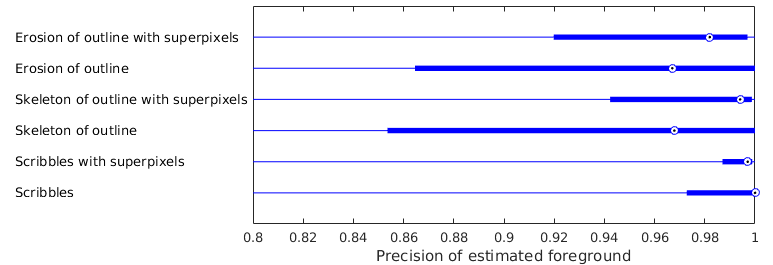
\includegraphics[width=\columnwidth]{assets/plot/precision_fg_all.png}
\caption{Precision of foreground user input}%
\label{fig:precision_fg}
\end{figure}


\begin{figure}[ht]
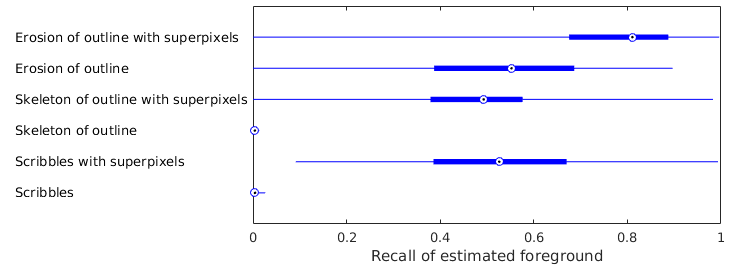
\includegraphics[width=\columnwidth]{assets/plot/recall_fg_all.png}
\caption{Recall of foreground user input}%
\label{fig:recall_fg}
\end{figure}


The precision of foreground area is given in
Figure~\ref{fig:precision_fg}, relatively to the ground truth masks.
We can observe that more than 75\% of foreground (green)
scribble inputs are over the 0.97 index.
This means that the task of scribbling inside the objects
is globally well performed but still slightly harder
than background (red) scribbles.
It is explained by the fact that objects can have thin shapes
and thus not precisely locatable under the finger
during the touch interaction.


Using the superpixels extension of the scribbles,
we observe that the smart background correction mentioned
in Section~\ref{sec:superpixels},
enhances the 75\% index to a precision of 0.99.
With the two foreground inference techniques (erosion and skeleton),
the improvement provided by the superpixels extension is obvious.


The recall of foreground area (Figure~\ref{fig:recall_fg})
provided by these interactions, extended through superpixels is
also coherent with what we observe in Figure~\ref{fig:foreground}.
Skeleton and scribbles recall values are almost 0 since they are of
dimension 0/1 (points/lines) for a measure of surfaces (dimension 2).
Erosion provides the most foreground information,
but has the lower precision rate (Figure~\ref{fig:recall_fg}).
We will show in the next section that this trade-off is worth exploring.


\subsection{Segmentation quality}


We computed the resulting segmentation of images using five different methods.
As a reference method, the mean Jaccard index obtained with foreground
and background scribbles is 0.79 (see table~\ref{tab:jaccard}).
When using the bounding boxes,
determining a clear background model input for the GrabCut algorithm,
the mean Jaccard increases to 0.82.
As expected, it increases even more when using outlining interaction inputs,
providing richer inferred initial foreground models to the GrabCut algorithm.
The higher scores (0.88 and 0.89) are respectively obtained when
using the erosion and skeleton processing of the outline.
The best performance is achieved using the skeleton processing,
which tends to show that for the results presented in the previous section,
the precision of the foreground user input is more important than its recall.


\begin{table}[ht]
\begin{tabular}{cccccc} \toprule
Method & Scrib. & B. Box & Outl. & Outl. + er. & Outl. + BMA \\ \midrule
\makecell{Mean\\Jaccard} & 0.79 & 0.82 & 0.86 & 0.88 & 0.89 \\ \bottomrule
\end{tabular}
\caption{Mean Jaccard index obtained on all images
for all users for each interaction}%
\label{tab:jaccard}
\end{table}


\begin{figure}[ht]
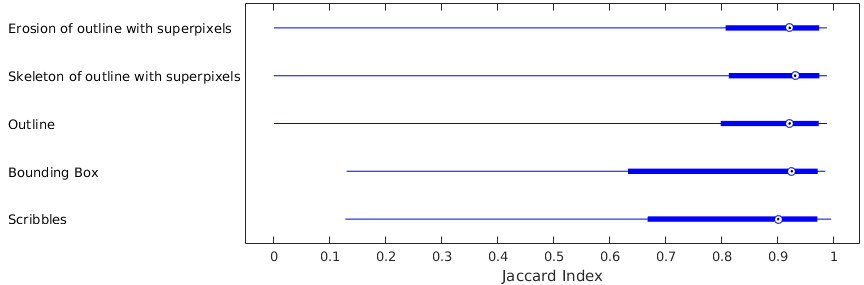
\includegraphics[width=\columnwidth]{assets/plot/jaccard.png}
\caption{Jaccard index obtained on all images for all users
for each interaction type. The dot represents the median value,
and the thick blue line limits the first and third quartiles.}%
\label{fig:jaccard}
\end{figure}


\begin{figure*}[ht]
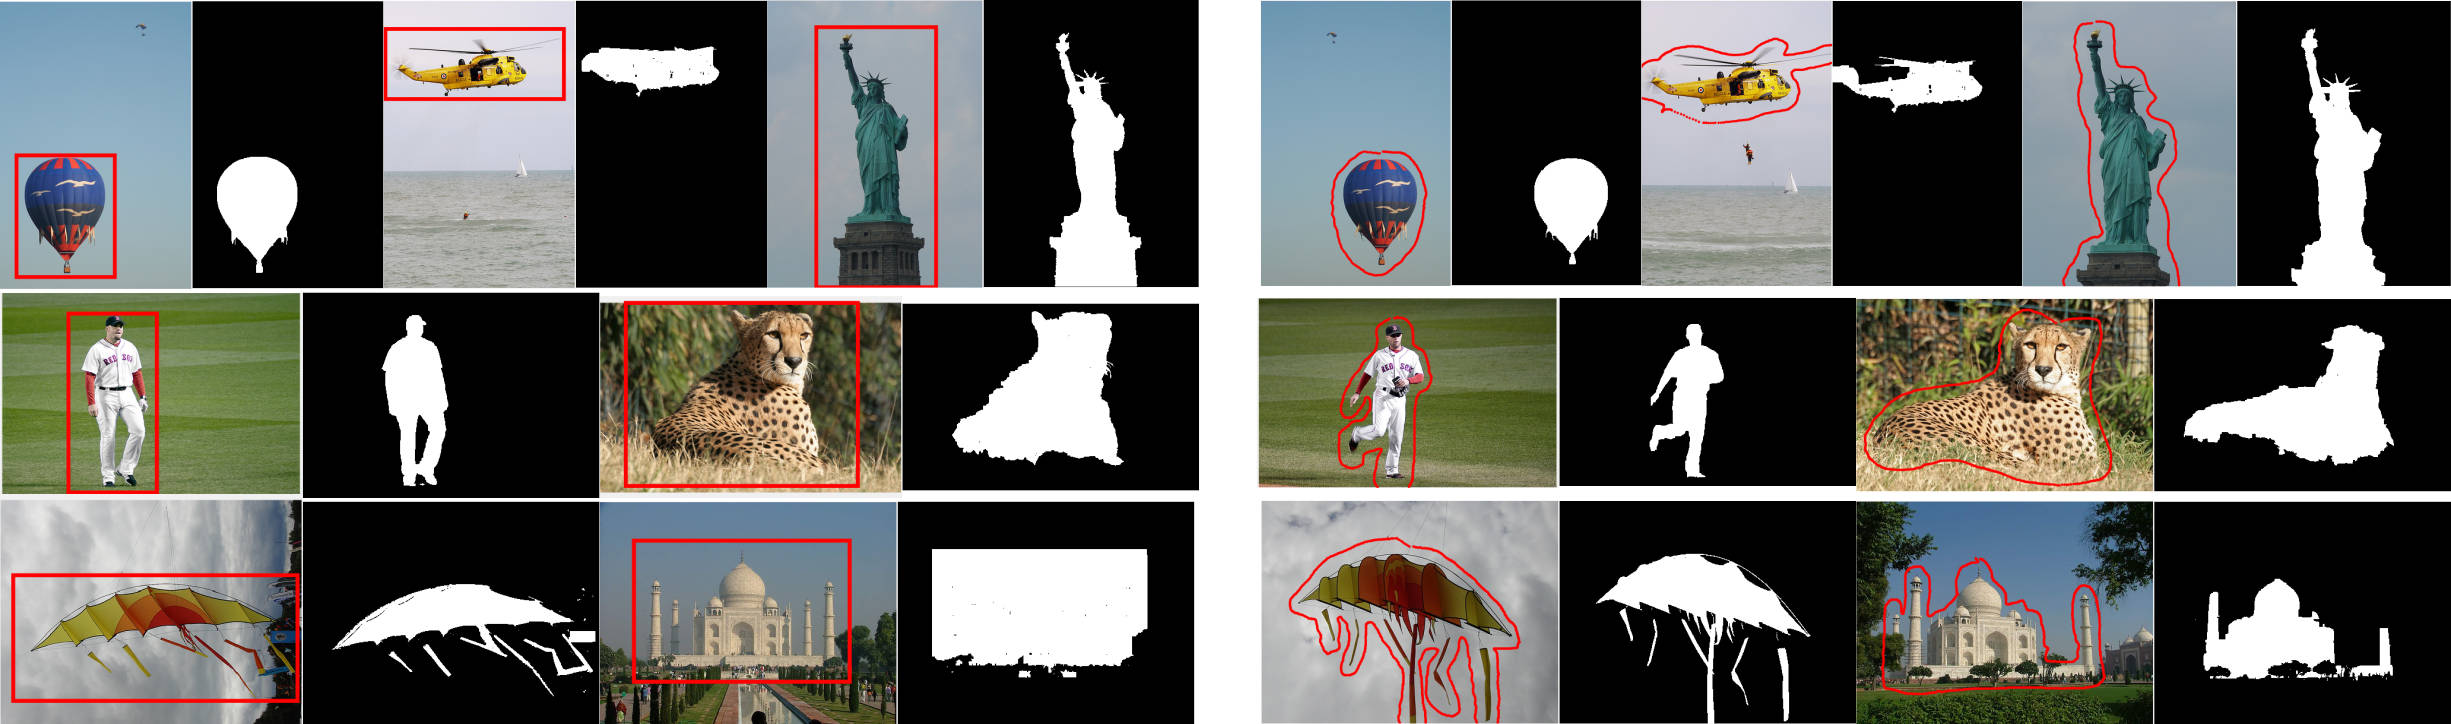
\includegraphics[width=\textwidth]{assets/img/results.jpg}
\caption{Segmentation results for bounding box
and outlining interactions from a single user.}%
\label{fig:results}
\end{figure*}


Perhaps more importantly, the outlining interaction enables reaching
consistently higher Jaccard index than the other techniques.
In Figure~\ref{fig:jaccard}, we observe that the first quartile is
always higher than 0.8 with variants of the outlining interaction.
Some final segmentation results are visible in Figure~\ref{fig:results}
and show the clear improvement brought by an outline over a bounding box.


\subsection{Discussion}


All the results we obtained confirm the good properties
of the outlining interaction, in the perspective of being used
in a segmentation crowdsourcing campaign.


First, it is a very straightforward interaction.
One of the users explained it in these terms:
\textit{outlining is easier since you do not need to think,
just trace the object.
Bounding boxes are tougher, particularly in determining a correct size,
and scribbles is too much thinking and a bit more time consuming.}
Another user said: \textit{It's actually more fun to draw around object
and would seem to me less tiring than the other methods}.
The usability criteria point out that outlining might be a little less
usable than drawing a bounding box,
and comparable to scribbling, but remains a very usable interaction.


Another interesting property of the outlining interaction
is the speed at which it can be performed.
Figure~\ref{fig:timeinteraction} shows that most of the outlines
were produced in less than 10 seconds,
which is very reasonable considering some of the images we chose have
complex shapes (see Figure~\ref{fig:complexoutlines}).


\begin{figure}[ht]
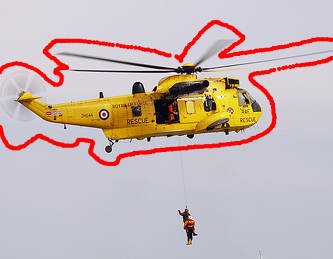
\includegraphics[width=0.31\columnwidth]{assets/img/helicopter_02_annot.jpg}\hfill
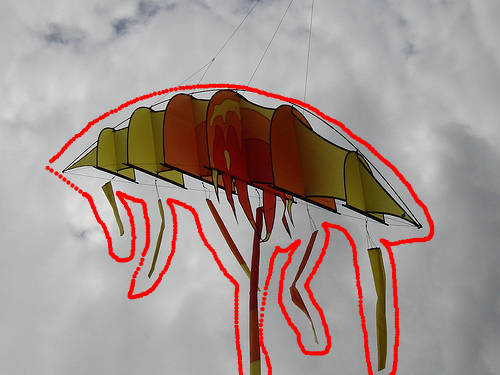
\includegraphics[width=0.32\columnwidth]{assets/img/kite_02_annot.jpg}\hfill
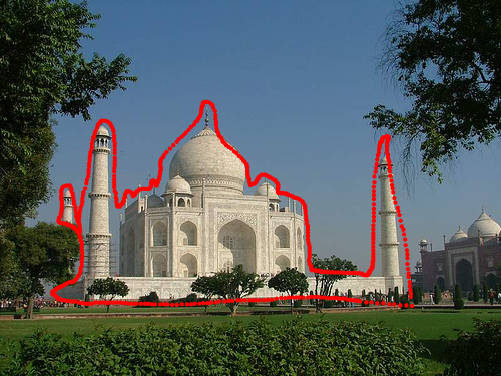
\includegraphics[width=0.32\columnwidth]{assets/img/taj_mahal_02_annot.jpg}
\caption{Outlines drawn by the third user on three images with complex shapes.}%
\label{fig:complexoutlines}
\end{figure}


The quantity of information brought by outlines is also very good,
as discussed in the previous section,
especially when compared with the interaction usability.
This information is of course less than a polygon drawn
on the boundary of the object (such as in LabelMe),
but can be augmented using computer vision techniques (Blum medial axis,
superpixels, GrabCut, etc.) and lead to very good segmentation masks.
The average Jaccard index value of 0.89 obtained with the outlines
is particularly impressive considering it was obtained
without any refinement, and in less than 10 seconds in average
(see for example the comparison with Jaccard index vs.\
time curves described in~\cite{carlier_clickncut:_2014}).


\section{Conclusion}


In this paper, we studied the outlining interaction
on touch devices for interactive segmentation.
We found that outlining is a simple and natural interaction, that allows
to quickly obtain a good information on the location of an object.
This information can be augmented with foreground inference,
and then used to compute a segmentation mask.
The segmentation masks obtained with this method reach an average
Jaccard index of 0.89, which is a very good result
considering the interaction does not require any knowledge
on image processing or computer vision from the user.


Because of all these good properties (simplicity, swiftness, accuracy),
outlining seems an interesting avenue to explore for the gathering
of large datasets of image segmentation masks.
Those datasets are crucial to bring the automatic image segmentation
algorithms, today mostly based on deep learning techniques, to a new level of effectiveness.
It is our intention to pursue this goal as a future work
and launch a crowdsourcing campaign to build such datasets.

\chapter{Reliable Web Applications}%
\label{cha:reliable_web_applications}

\begin{itemize}
	\item What is the Web?
	\begin{itemize}
		\item What is a Web application?
		\item Rich Internet Application (RIA)?
	\end{itemize}
	\item JavaScript or ECMAScript
	\begin{itemize}
		\item Creation of JavaScript
		\item Browser performance war with Just In Time compilation (JIT)
		\item Explosion of JavaScript and Node
		\item JavaScript issues
		\item The ``transpilation to JavaScript'' paradigm
	\end{itemize}
	\item Frontend Web programming
	\begin{itemize}
		\item Single Page Application (SPA)?
		\item Reactive programming
		\item Functional Reactive programming (FRP)
		\item About the Virtual DOM
		\item Async and the event loop
	\end{itemize}
	\item Elm
	\begin{itemize}
		\item Pure functions
		\item Algebraic Data Types (making impossible states impossible)
		\item Totality
		\item Switch to The Elm Architecture (TEA)
		\item 0 runtime exception
		\item Elm-UI, an alternative layout approach
	\end{itemize}
\end{itemize}


\section{What is the Web?}%
\label{sec:web}

The Internet and the Web are ubiquitous technologies of our everyday lives,
created \comment{around the 80's.}{would be good to be more precise}
Social media, communication, search, news, entertainment, mapping,
shopping, learning, \replace{allmost every}{virtually any} activity is now digital and online.
Simply put, the Web, also called World Wide Web (WWW), consists of the sum of all resources,
available through unique identifiers (URI), that we share on the Internet,
the global network carrying them.

In this chapter, we will recap the Web main evolutions,
from static content to dynamic applications,
and explain the choices we made to build reliable annotation Web applications.

\subsection{What is a Web application?}%
\label{sub:web_application}

An application, in the context of programming (/computers),
is a piece of software presenting information to a user,
usually in an actionable manner.
This includes \replace{things}{programs} like email clients, image \replace{manipulation}{editors}, video games,
word processors, automatic \replace{translation}{translators}, and virtually any functionality
available on a regular computing device.

Web resources are commonly accessible through a Web browser.
Thus, we can define a Web application as a user-facing software,
accessed through a Web browser.
As of May 2019 according to statcounter~\cite{browser-market-share},
the most used Web browsers are Google Chrome (62.7\% of global market share),
Apple Safari (15.9\%) and Mozilla Firefox (5.1\%).

The three pillars of Web applications are HTML, CSS and JavaScript.
HTML, for ``Hypertext Markup Language'' is a description language
organizing a page information as a hierarchy of tagged content.
In Listing~\ref{lst:html}, a ``body'' tag contains three other tags,
a title ``h1'' (h for header), a paragraph ``p'', an image ``img''
and a button not yet linked to any action.
This hierarchical organization of an HTML page is call the DOM,
for Document Object Model.
CSS, for ``Cascading Style Sheet'', complements HTML by styling
the content of associated HTML documents.
Listing~\ref{lst:css} shows how \replace{we}{one} would add a left margin of 20 pixels
on all the document body, and make the h1 title red and bold.
\add{Finally, }JavaScript is a scripting language, not affiliated in any form
to the Java programming language.
It is run inside the browser to add dynamic behavior to a Web page.
In Listing~\ref{lst:js} we show how one could count and display
the number of times a user clicked on the button in the page.

\lstinputlisting[language=HTML,caption={Example HTML code.},label={lst:html}]{assets/code/html.html}
\lstinputlisting[language=CSS,caption={Example CSS code.},label={lst:css}]{assets/code/css.css}
\lstinputlisting[language=ES6,caption={Example JavaScript code.},label={lst:js}]{assets/code/js.js}

\subsection{Rich Web Application}%
\label{sub:rich_web_application}

Traditionally, websites used to present their resources in the form of a collection
of static documents, known as Web pages, linked together with hyperlinks.
The nature of Web pages would mostly be informative, visual or textual,
with very few other interactions than navigation through the site by
clicking on the links.

Today, thanks to evolutions of Web technologies that we will detail later,
Web applications have become full-fledged applications with almost
the same capabilities as desktop ones.
They feature functionalities like 3D graphics, \replace{sound}{audio} processing or interactive elements,
and are sometimes called rich web applications.
Similar concepts like ``progressive web applications'' (PWA),
or ``single page applications'' (SPA) are also explained in the following sections.
In the next section, we will dive into the cornerstone of Web pages dynamism, JavaScript.


\section{JavaScript, formally known as ECMAScript}%
\label{sec:javascript_formally_known_as_ecmascript}

\subsection{Genesis of JavaScript}%
\label{sub:genesis_of_javascript}

In 1995, the dominating Web browser was the Netscape Navigator.
Realizing that pages dynamism was key in the \replace{war}{competition} against Microsoft\add{'s}
own Web technologies, Netscape Communications recruited Brendan Eich,
with the aim of integrating a scripting language into their browser.
\replace{And so, in May 1995, he wrote a prototype in 10 days.}{A first prototype was thus developed in 10 days (May 1995).}
Assumably for marketing reasons, it was officially named JavaScript
when released in Netscape Navigator 2.0 beta 3.

Two years later, in June 1997, the European Computer Manufacturers Association
(ECMA) standardized the first version of ``ECMAScript'' as ECMA-262,
JavaScript being its most well\add{-}known implementation.
The ECMAScript (ES) standard has been evolving \add{ever} since.
Today, all browsers fully implement ES5, released in 2009,
and partially implement the most recent versions, ES2015,
ES2016, ES2017 and ES2018.

\subsection{Browser performance war}%
\label{sub:browser_performance_war}

Many browser wars for dominance of market share occurred since the 90's.
\add{In this section, }we are \add{particularly} interested in the JavaScript engine performance war,
starting around 2008 when Google released its Chrome browser.
On September 2, 2008, Google announced a new Web browser called Chrome~\cite{google-chrome}.
Its main selling \replace{point}{feature} was a new JavaScript engine called V8,
greatly improving the browser performances on web applications making
heavy use of JavaScript like their email client \comment{Gmail}{should we notify trademarks with a proper style?}.
\replace{Beware}{Note} that ``performance'' in a browser \replace{is the result of}{depends on} many factors
such that network latency, DOM computation, page rendering or JavaScript processing.
In this section, we will specifically focus \add{on} JavaScript execution performances.

\subsubsection{Dynamic interpretation}%
\label{ssub:dynamic-interpretation}

\replace{Previously, JavaScript was}{JavaScript was originally} an interpreted language.
For each line of code, the engine would translate it into machine code,
and immediately execute it.
This means that for a loop, the \add{same} transformation from JavaScript to machine code
is repeated over and over again.
In addition, JavaScript is a dynamic language, which is \add{both} one of its
strongest points but also a \replace{nightmare for}{huge drag on} execution.
Let's take the function adding two numbers \add{depicted in Listing~\ref{lst:add-js}} as an example
\remove{as in Listing}.

\lstinputlisting[language=JavaScript,caption={Adding two values.},label={lst:add-js}]{assets/code/add.js}

\comment{}{If what follows is a quote, it should be made clearer in the presentation.}
\begin{displayquote}
According to the ECMAScript specification~\cite{ecmascript},
the addition operator either performs string concatenation or numeric addition.
The production ``AdditiveExpression : AdditiveExpression + MultiplicativeExpression''
is evaluated as follows:

\begin{enumerate}
    \item Let lref be the result of evaluating AdditiveExpression.
    \item Let lval be GetValue(lref).
    \item Let rref be the result of evaluating MultiplicativeExpression.
    \item Let rval be GetValue(rref).
    \item Let lprim be ToPrimitive(lval).
    \item Let rprim be ToPrimitive(rval).
    \item If Type(lprim) is String or Type(rprim) is String, then
    \begin{enumerate}
        \item     Return the String that is the result of concatenating ToString(lprim) followed by ToString(rprim)
    \end{enumerate}
    \item Return the result of applying the addition operation to ToNumber(lprim) and ToNumber(rprim). See the Note below 11.6.3.
\end{enumerate}

\textbf{NOTE 1}. No hint is provided in the calls to ToPrimitive in steps 5 and 6. All native ECMAScript objects except Date objects handle the absence of a hint as if the hint Number were given; Date objects handle the absence of a hint as if the hint String were given. Host objects may handle the absence of a hint in some other manner.

\textbf{NOTE 2}. Step 7 differs from step 3 of the comparison algorithm for the relational operators (11.8.5), by using the logical-or operation instead of the logical-and operation.
\end{displayquote}


In theory, if we know that we will only use this function
to sum two numbers, it should compile to a single instruction.
However, due to the dynamic nature of JavaScript,
as specified in the standard, the code has to check if the arguments
are strings, objects, and proceed first with conversions before
eventually reaching the instruction \replace{doing}{that actually computes} the addition.
This process results in one or two orders of magnitude slower code,
compared to statically typed languages like C or Java.

\subsubsection{Just-in-time (JIT) compilation}%
\label{ssub:just_in_time_jit_compilation}

Statically typed languages usually compile code ahead-of-time (AOT),
while dynamically typed languages interpret code at runtime.
Starting with Chrome in 2008, all browser vendors began implementing
just-in-time (JIT) compilers.

The key ingredient is a ``monitor'' sometimes called ``profiler''.
The monitor watches the code while it is run by the interpreter,
and keeps track of how often a piece of code is executed.
Once a path of code is \add{found to be }repeatedly executed, it becomes ``hot'',
which triggers an optimizing compiler.
According to the types previously used in the hot path,
the optimizing compiler will make assumptions enabling
extremely efficient machine code.
If the same code is used once with different types however,
it gets de-optimized back to the baseline compiler.
Multiple optimization and de-optimization round trips
hinders the performances, and consequently will permanently mark
the section as not to be optimized anymore.
For more information on JIT compilation, Lin Clark~\cite{clark-jit}
wrote an \add{enlightning} introductory blog post.

Figure (\alert{TODO faire un schema timeline}) outlines the differences between
interpreting and JITing regarding the ratio of time spent on each phase.
\comment{Fun fact, in V8 the baseline compiler and interpreter is known as ``Ignition''
and the optimizing compiler goes by the name of ``TurboFan''.}{This can probably be ignored :-)}

\comment{}{List of links commented in code}
% December 18, 2007 - https://webkit.org/blog/152/announcing-sunspider-09/
% December 19, 2007 - https://blog.codinghorror.com/the-great-browser-javascript-showdown/
% September 2, 2008 - https://blog.chromium.org/2008/09/google-chromes-need-for-speed_02.html
%  -> release date of Chrome
% September 3, 2008 - https://johnresig.com/blog/javascript-performance-rundown/
% September 3, 2008 - https://arstechnica.com/information-technology/2008/09/new-firefox-javascript-engine-is-faster-than-chromes-v8/
% September 5, 2008 - https://www.zdnet.com/article/is-firefox-faster-than-chrome/
% September 19, 2008 - http://www.satine.org/archives/2008/09/19/squirrelfish-extreme-fastest-javascript-engine-yet/
% November 14, 2008 - https://allanfeid.com/content/javascript-engine-benchmark-test-results
%
% SunSpider: JS perf test suite by WebKit team
% https://www2.webkit.org/perf/sunspider/sunspider.html
% no longer maintained -> cf JetStream
%
% JetStream: Test JS and wasm
% https://browserbench.org/JetStream/
%
% V8 Benchmark: heavy emphasis on recursion


\subsection{Explosion of JavaScript}%
\label{sub:explosion_of_javascript}


\subsubsection{Node.js}%
\label{ssub:node_js}

Not long after the release of the V8 engine from Google,
Ryan Dahl announced at the European JSConf of 2009
a new project named \comment{node.js}{not Node.js ?}~\cite{node-js-speaker}.
As he explains in his talk~\cite{node-js-video},
node is a cross-platform JavaScript runtime environment based on V8.
It features an event-driven architecture, with non-blocking input/output (I/O) APIs.
The project matured from the observation that blocking I/O is extremely non-efficient,
since it requires many threads and \replace{much}{a large} memory to scale with connections.
\remove{JavaScript} Being event-driven by nature in the browser,
\replace{it}{JavaScript} was a perfect fit for the node project.

In order to provide non-blocking asynchronous I/O,
node is composed of an event loop managing callbacks in queued fashion,
and of a thread pool, executing all blocking I/O calls like file reading.
Both are abstracted away by the system, and so a user simply has
to provide callbacks that will automatically be run upon completion of I/O \add{calls?}.
An example of reading a file is presented in Listing~\ref{lst:read-file-js}.

\lstinputlisting[%
	language=JavaScript,
	caption={Read a file with node.js.
		Notice the event-driven architecture with an anonymous callback function passed as argument.},
	label={lst:read-file-js}
]{assets/code/readFile.js}


\subsubsection{Node package manager (npm)}%
\label{ssub:node_package_manager_npm_}

\begin{displayquote}
	\textit{``To increase speed, you can either push harder or reduce friction.''}
	--- Isaac Z. Schlueter, node.conf, Portland, OR, May 5th, 2011
\end{displayquote}

With the rise of node for server-side JavaScript,
another highly influencial project was born late 2009, \add{the Node package manager} (npm).
Isaac Z. Schlueter, while working at Yahoo, wanted to increase usage
of JavaScript for full stack web development.
According to him, many people were already pushing hard on node.js,
so he \comment{took a stab}{trop familier} at lowering friction by creating the Node Package Manager (npm).
The core design choices of npm are rooted in the principle of reducing
most sources of friction, including the following:

\begin{itemize}
	\item \textbf{Conflicting dependencies.}
		When transitive dependencies require different versions of the same package.
		As a consequence, npm retrieves every version needed by dependencies.
	\item \textbf{Inconsistent package installation.}
		Typically, one would need to clone, make, copy, rename files, etc.
		With \verb|npm install|, dependencies are all installed locally,
		under the \verb|node_modules/| directory and usable by invoking
		\verb|require('the-module')|.
	\item \textbf{Publishing difficulties.}
		Usually, package registries require a lot of metadata.
		Npm only requires two fields, name and version.
\end{itemize}

% Mention inspiration from Yahoo's yinst package manager?
% https://www.reddit.com/r/npm/comments/aounfi/best_package_manager/

As a result, npm grew exponentially, to become the world's largest package
registry ever, by a large amount, with over a million packages since June 2019.
At node.conf 2011~\cite{npm-video}, when Isaac Schlueter announced npm 1.0,
the registry contained 1900 packages and almost 800 active package authors.
This roughly corresponds to doubling the registry size every year!

Unfortunately, reduced friction and a policy favoring package creators over users
brought a few security issues.
The most notable one is probably the event-stream incident late 2018~\cite{npm-event-stream}
where a new maintainer of the event-stream package added a dependency
to a malicious package, harvesting bitcoin from visitors of a targeted application.
We will discuss later how this risk is reduced with elm packages.


\subsection{JavaScript issues}%
\label{sub:javascript_issues}

\subsubsection{Organic growth and backward compatibility}%
\label{ssub:organic_growth_and_backward_compatibility}

Most programming languages tend to grow in complexity with time.
New features are regularly added, and backward compatibility requires that
\replace{old ways of doing things}{outdated practices} are kept in the language.
JavaScript is a good illustration of this kind of organic growth.
As an example, the language specification of JavaScript is 805 pages~\cite{ecmascript-pdf}.
This is roughly the same size as the Java specification with 772 pages~\cite{java-spec-pdf}
or the C specification with 571 pages~\cite{c-spec-pdf}
To compare, the specification for the Go progamming language
by Google~\cite{go-spec}, contains approximately 100 pages.

\comment{}{Plus tard mettre citation, it will be finished when there is nothing left to remove.}

The \replace{wildest}{most salient} evolutions occurred with ES2015 (previously known as ES6).
\comment{Among the confusing ones for beginners are the ``const'' and ``let'' keywords.}{tournure bizarre}
They introduce two new ways of declaring variables, bringing it to a total of four,
along with the ``var'' keyword and no keyword.
Differences between those are presented in Listing~\ref{lst:var-scope-js}.

\lstinputlisting[language=ES6,caption={Variable scope in JavaScript.},label={lst:var-scope-js}]{assets/code/var-scope.js}

\comment{The syntax list continues with ``arrow functions'', ``promises'' and so on.
Most new features are illustrated online at es6-features.org,
I suggest browsing this site for more information.}{Je ne suis pas sur de l'utilit\'e de ces phrases. A remplacer peut-etre par un commentaire sur la complexit\'e de ces keywords, ou une comparaison avec d'autres langages ?}

\comment{}{%
	Il pourrait être aussi intéressant de montionner les choses suivantes :
	- Module systems (CommonJS, AMD, ES2015): https://auth0.com/blog/javascript-module-systems-showdown/
	- ESNext (generators, observers, ...)
}

\subsubsection{Callback hell}%
\label{ssub:callback_hell}

As mentioned when introducing node.js,
JavaScript event-driven APIs rely on callback functions.
Let's consider a simple case where we want to retrieve information
from a database.
Listing~\ref{lst:callback-hell-sync} outlines how a blocking synchronous API
would look like.
The control flow of the program is easy to follow,
but blocking at ``getDatabase'' and ``db.get'' calls
means the server (or the graphical interface) is \replace{non}{not} responding
during this time.

\lstinputlisting[%
	language=ES6,
	caption={Hypothetical blocking and synchronous API.},
	label={lst:callback-hell-sync}
]{assets/code/callback-hell-sync.js}

In contrast, the asynchronous callback version
in Listing~\ref{lst:callback-hell-callback},
is efficiently giving back control while waiting for the
database to connect and respond.
The main drawback resides in the complexity of the control flow,
and the verbosity of the code.
By a convention that emerged with time,
callback functions are supposed to handle a potential error
as first argument, and successful result as second argument.
This model \comment{continues to bring suffering to JavaScript developers}{cela semble une assertion forte, et je n'en vois pas trop l'origine dans les lignes pr\'ec\'edentes},
and thus has been coined in the community the ``callback hell''~\cite{callback-hell}.

\lstinputlisting[%
	language=ES6,
	caption={Typical asynchronous API based on callbacks.},
	label={lst:callback-hell-callback}
]{assets/code/callback-hell-callback.js}

We should mention that recent JavaScript standards provide new syntax
making use of ``async'' and ``await'' keywords to simplify
the control flow, while preserving the performances of
the callback model.
Listing~\ref{lst:callback-hell-async} shows how the same code can take advantage of the new syntax.
Unfortunately, this is to the detriment of language simplicity,
as explained in the previous point.

\lstinputlisting[%
	language=ES6,
	caption={Asynchronous version with the new async/await syntax.},
	label={lst:callback-hell-async}
]{assets/code/callback-hell-async.js}

\subsubsection{Context of this}%
\label{ssub:context_of_this}

In other object-oriented languages,
``this'' (or ``self'') usually refers to the currently used instance of a class.
As defined in the specification,
\textit{The this keyword evaluates to the value of the ThisBinding of the current execution context.} \comment{}{j'avoue que je ne comprends pas trop la phrase en italique}
JavaScript not being a typical object oriented language,
``this'' can take many shapes, depending on the execution context.
The execution contexts are in a stack in which new contexts are created and pushed
whenever code not associated with the current context starts running.
This typically happens in function calls.
Let's take Listing~\ref{lst:this-js} to exhibit some oddities of the ``this'' value.

\lstinputlisting[%
	language=ES6,
	caption={Value of ``this'' in JavaScript.},
	label={lst:this-js}
]{assets/code/this.js}
\comment{}{Honnetement, j'ai rien compris de cette partie :-(}
By default, if ``this'' is undefined, as in lines 17 and 18,
it is binded to the global object.
At line 11, we define ``x = 1'' with no keyword,
so ``x'' is a global variable.
As a result, line 17 and 18 print 1.
The definitions of the ``log'' and ``logF'' methods on the ``Who'' class
lines 7 and 8 are equivalent. The behavior of ``this'' in that context,
is what we expect to see for methods call on objects and thus,
lines 20 and 21 both print 2.
The ``call'' function (and some others), used for the definition of the ``logCall'' method,
enables binding of the ``this'' value to a specific object given as first argument.
That is why line 23 prints 3.

Now the most surprising results are lines 19 and 22, both printing 1 instead of 2.
At line 13, ``logMe'' is defined as the same function than ``me.log'' which
actually is the original ``log'' function.
As a consequence, line 19 is strictly equivalent to line 18, and they both print 1.
Finally, the ``logF2'' method also prints 1 because it's definition isn't the log function
(as defined for the ``log'' method) but rather calls the ``log'' function which
generates another context in which ``this'' is not defined anymore.
The behavior is thus the same than for lines 17 and 18, which binds ``this'' to the global object,
and prints the global variable ``x = 1''.

\subsubsection{Dynamic typing and implicit conversions}%
\label{ssub:dynamic_typing_and_implicit_conversions}

JavaScript is a dynamically typed language.
This means that types of values are only known at runtime,
and that they can change during the execution of the program
as shown in Listing~\ref{lst:dynamic-js}.

\lstinputlisting[%
	language=ES6,
	caption={Dynamic typing in JavaScript.},
	label={lst:dynamic-js}
]{assets/code/dynamic.js}

In addition, JavaScript performs implicit conversions between type,
depending on the operators and functions being used.
In Listing~\ref{lst:weak-js}, the number 42 gets converted into the string ``42''
before concatenation, and the string ``6'' is converted to the number 6
before multiplication with the number 7.

\lstinputlisting[%
	language=ES6,
	caption={Weak typing in JavaScript (implicit conversion).},
	label={lst:weak-js}
]{assets/code/weak.js}
\comment{}{3e exemple ajout\'e grace \`a tforgione}
By combining dynamic types, and implicit conversions,
JavaScript often generates extremely surprising situations,
resulting in unexpected behaviors.
It can also lead to very original use cases.
In 2010, an informal code obfuscation competition resulted in the creation
of a subset of JavaScript containing only six characters~\cite{jsfuck},
``['', ``]'', ``('', ``)'', ``!'' and ``+'',
able to represent any valid JavaScript code.
The value ``false'' would be obtained with ``![]'',
since negation of an empty array returns ``false'' according to JavaScript specification.
Numbers, characters, and other language constructs are obtained through similar
implicit conversion tricks.

\subsubsection{Undefined is not a function}%
\label{ssub:undefined_is_not_a_function}

\begin{figure}[ht]
	\centering
	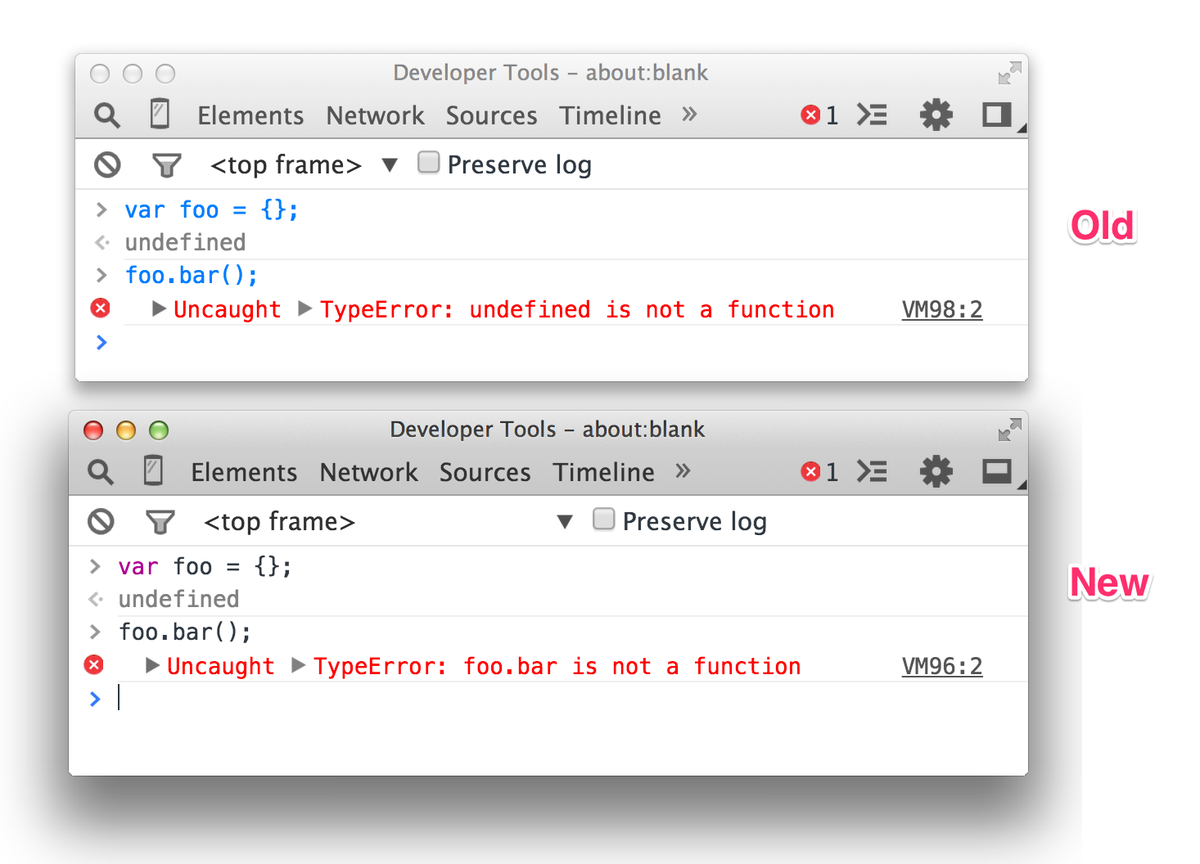
\includegraphics[width=1.0\linewidth]{assets/img/undefined-improved.png}
	\caption{Tweet by Addy Osmani (21-Feb-2015) announcing error report improvements in Chrome.}%
	\label{fig:undefined-improved}
\end{figure}

For JavaScript developers previous to 2015,
the error ``undefined is not a function'' was \comment{famous for not being helpful}{n\'ecessite une r\'ef\'erence}.
This error would very often rise from a typo somewhere in the code.
Due to the dynamic nature of JavaScript, the error can be reported late in the call stack.
Indeed, even if an error in the code might create an ``undefined'' value,
it is only later when called, that an uncaught error would trigger.
As shown in Figure~\ref{fig:undefined-improved}, browsers are more helpful now,
at the cost of loosing an iconic error for all JavaScript developers.
Yet not having a compile step prevents advanced static analysis of the code,
and at the same time lengthen the feedback loop to fix errors.


\subsection{JavaScript as a compilation target}%
\label{sub:javascript_as_a_compilation_target}

As we now know, JavaScript exists since 1995, and from 1997 onward,
has mostly been the only way to run code dynamically in the browser.
For this reason, many alternative languages started treating JavaScript
as a compilation target to run code in a browser.

\subsubsection{Multi-tier programming}%
\label{ssub:multitier}

Haxe was probably the first production ready language to target JavaScript, in 2006.
At this time, there was no JIT, and JavaScript performances were \replace{n't great either}{fairly limited}.
\remove{Yet s} \add{S}ome people were \add{nonetheless} trying to make the Web a video and gaming platform.
Flash, a multimedia platform running the ActionScript language was the \replace{rising star}{most popular solution} at the time.
In 2005, YouTube \replace{made use of}{was for example relying on} a Flash player to distribute videos.
Haxe was created by Nicolas Cannasse~\cite{haxe-interview} with the clear purpose to remove the overhead of composing heterogeneous components like a Flash client,
a Web server, and additional JavaScript \remove{glue} \replace{when designing Web games}{for Web games design}.

Many other languages \add{later} followed that \replace{trend}{path} of using the same language
for server and client code, sometimes called ``isomorphic'' frameworks.
Google announced their Google Web Toolkit (GWT) in May 2006~\cite{gwt},
enabling Java developers to build client applications.
The Ocsigen framework by V. Balat et al.~\cite{balat2006ocsigen} in 2006
allowed building fully featured applications in the OCaml programming language.
The Opal compiler~\cite{opalrb} \replace{transforms}{translates} ruby code into JavaScript,
\comment{enabling full stack Ruby with the rails framework for the backend.}{too technical, to be made clearer; what is rails ?}
Today, most programming languages can target JavaScript,
including Python, C, Erlang, Haskell, etc.

Around the same period, academic research \replace{is}{has} also \add{been} trying to solve
what we call \comment{multi-tier web programming}{to be defined ??} with unique new languages like Links
by E. Cooper et al.~\cite{cooper2006links},
or Hop by Serrano et al.~\cite{serrano2006hop} in 2006.
Those efforts are continuing with for example
A. Chlipala et al.~\cite{chlipala2015ur} who created the Ur/Web variant
of the Ur modelling language,
or Sinha et al.~\cite{sinha2015simplifying} with the WebNat programming language in 2015.
Unfortunately, those research attempts at novel ways of programming the Web
are not \add{yet} adopted by \replace{the programmers}{developers}.
According to~\cite{sinha2015simplifying},
one of the key \comment{factors}{factors of what? of not adopting multi tier programming? if so, to be made clearer}   is that experienced Web programmers want fine grained
control on the generated code for designing complex applications.

\subsubsection{JavaScript as the main target}%
\label{ssub:javascript_as_the_main_target}

Instead of trying to tackle both server and client-side programming,
a new category of languages later emerged, focusing on the client side,
and with JavaScript being the only or main compilation target.
The most notable ones are CoffeeScript~\cite{coffeescript} released in 2009
by Jeremy Ashkenas, Dart~\cite{dart-blog} designed by Lars Bak
(creator of the V8 engine) and Kasper Lund for Google in 2010,
Elm~\cite{czaplicki2013asynchronous} the product of Evan Czaplicki senior thesis
on functional reactive programming in 2012,
and Reason~\cite{reason} (also known as ReasonML) in 2016 by Jordan Walke (who is
also the original designer of the React framework we will discuss later).

One can notice that appart from Dart, which is heavily object-oriented,
those new languages \remove{for the client} follow the functional paradigm.
\comment{It is not estranged}{TODO : check this expression} from guaranties brought by
functional programming that we will develop when exploring the Elm programming language.

\comment{A note about the Dart language, it has been abandonned for Web programming,
but found a new home in the Flutter framework%~\cite{flutter}
, released in 2017,
targeting mainly native development of mobile applications on iOS and Android.}{pas certain que ce soit utile}

\comment{}{sur cette section je reste un peu sur ma faim ; tu listes des frameworks, tu dis qu'ils sont fonctionnels pour des raisons qu'on d\'etaillera plus tard mais cela apporte finalement assez peu d'info}

\subsubsection{Gradually typed JavaScript}%
\label{ssub:gradually_typed_javascript}

Coding with a completely different language is a rather extreme approach
which can \replace{feel overwhelming}{be disturbing for developers}.
From this observation, both Microsoft and Facebook decided to bring
new contributions to the JavaScript ecosystem \replace{in}{under} the form of gradual typing.
Gradual typing is a type system where values are partially typed.
Some may be typed, and consequently static typing rules are verified,
and some may be untyped, left for compile-time verifications.

In October 2012, Microsoft released TypeScript~\cite{bierman2014understanding},
a superset of JavaScript, \replace{enabling}{introducing} \comment{}{ajouter "facultatif", ce qui explique la prochaine phrase}  type annotations.
As a consequence, any valid JavaScript program is also a valid TypeScript program.
This property was most certainly the major success factor of TypeScript.
Programs can be \comment{ported}{TO BE CHECKED} progressively to benefit from static analysis.
Listing~\ref{lst:add-ts} exhibits the core type annotation feature of TypeScript.

\lstinputlisting[%
	language=JavaScript,
	caption={JavaScript and TypeScript version of an add function.},
	label={lst:add-ts}
]{assets/code/add.ts}

Another benefit of static typing that JavaScript developers are discovering when
switching to TypeScript is the improved IDE support,
with \add{includes for example} better autocompletion tools, jumping to definitions \replace{and other support from your editor}{etc}.

In 2014, another tool named Flow and led by Facebook~\cite{chaudhuri2017fast}
enabled gradual typing of JavaScript.
Ultimately, TypeScript seems to \replace{have taken the biggest part of the cake}{be the most popular one},
but choosing between the two will most likely depend on how well they integrate
with \comment{your working framework}{tournure non standard pour un manuscrit de these}.

\subsubsection{JavaScript transpilation}%
\label{ssub:javascript_transpilation}

Despite increasing language complexity
as explained in Section~\ref{ssub:organic_growth_and_backward_compatibility},
ES2015 and later specifications brought very appreciated \add{new} features \remove{to the table},
\replace{many}{often} influenced by other languages like CoffeeScript.
The ``async / await'' pair of keywords is such example of syntax
\comment{improving on complexity}{pas clair : improving ou increasing} of the code control flow.
New specifications, however, are not always immediately available in all browsers,
especially mobile versions.
But there \replace{is}{exists} one version of JavaScript fully supported on all browsers, ES5.
Inspired by the \comment{traceur}{TO BE CHECKED} tool by Google engineers,
Sebastian McKenzie \comment{jumped head first}{trop familier} into writing 6to5~\cite{babel}
on September 2014, at the age of 17.
His 6to5 project, now renamed Babel, is known as a JavaScript ``transpiler'',
i.e.\ a program converting recent JavaScript source code into another (older) version
of JavaScript source code.
Today, Babel has become one of the most used tools
with 7 million weekly downloads on npm.


\section{Frontend Web programming}%
\label{sec:frontend_web_programming}


\subsection{Single Page Application (SPA)}%
\label{sub:single_page_application_spa_}

In a desire to improve user experience in Web applications,
code location has been shifting from server to client.
Since 2009, a Web framework named AngularJS~\cite{hevery2009declarative} strongly pushed
the Web actors toward writing ``Single Page Applications'' (SPA).
A Single Page Application gets its name from the fact that only one
HTML page is sent to the client browser.
This page however, contains JavaScript code taking control
of the application and rendering it for the rest of the user navigation.
When new data is required, the application can send requests
with the XMLHttpRequest (XHR) object, or a WebSocket provided by the browser,
then process the answer and re-render the HTML page accordingly.
Since February 2005, this technique was popularized under the name Ajax~\cite{ajax}
by Jesse James Garret and is represented in Figure~\ref{fig:spa}.
Ajax stands for asynchronous JavaScript and XML,
though today exchanged data is mostly in the JSON format (JavaScript Object Notation) instead of XML,
and occasionally just raw bytes depending on use cases and protocols.
Let's describe briefly today's leading Web frameworks, namely Angular, React and Vue.

\begin{figure}[ht]
	\centering
	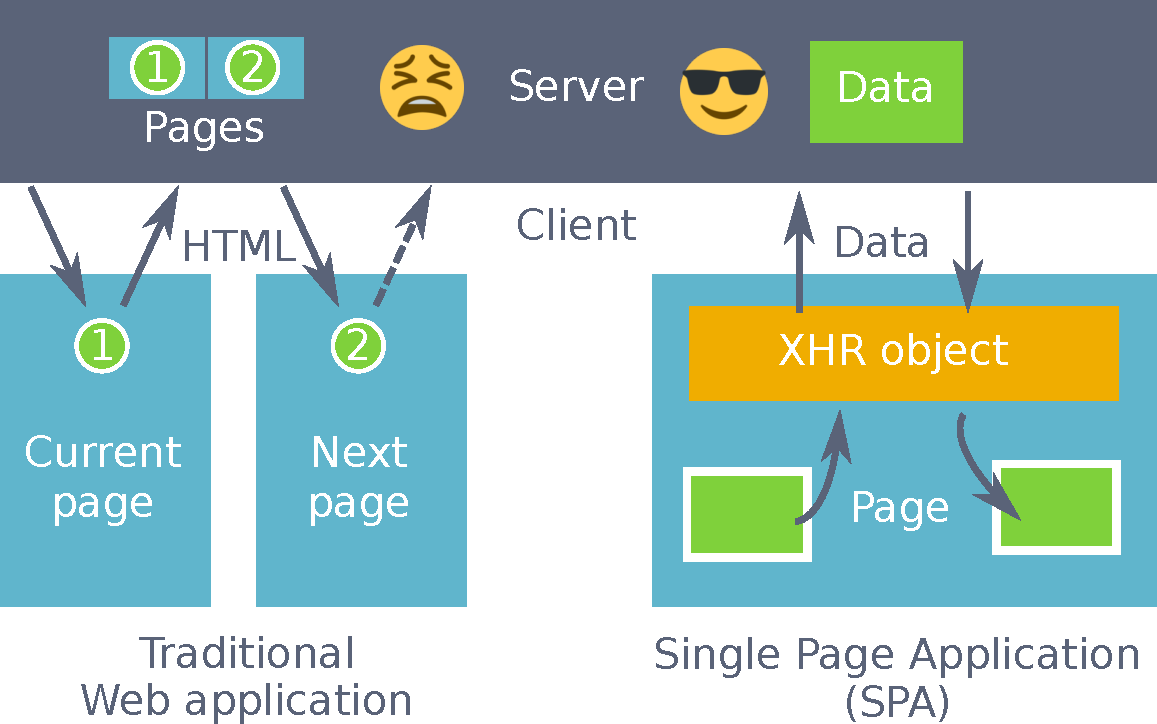
\includegraphics[width=1.0\linewidth]{assets/img/spa-bis.pdf}
	\caption{Difference between traditional Web applications and Single Page Application (SPA). A traditional application will ask the server to generate a new HTML page to access the required content. A SPA will just ask for the required data and render it in the client directly.}%
	\label{fig:spa}
\end{figure}

\subsubsection{Angular}%
\label{ssub:angular}

AngularJS~\cite{hevery2009declarative} goes back to 2009, when Miško Hevery and Adam Abrons
where trying to sell online storage services through software at getangular.com.
The project wasn't successful enough, and so they made <angular/> open source.
Miško Hevery was later recruited at Google, working on their feedback project.
The story, as told by Miško Hevery and Brad Green at Google I/O 2013~\cite{angularjs-googleio},
says that it took Miško three weeks (though he had bet two) to rewrite a six-month work
with 17000 lines of code into 1500 lines of code with <angular/>.
Impressed, Brad decided to embrace the <angular/> project under Google's wing
and it got rebranded AngularJS with a new logo.
In 2016, Google released its successor, renamed Angular (without the JS part).
An important difference is that Angular is using TypeScript instead of JavaScript.
The key feature of Angular/AngularJS is declarative two-way data binding,
showcased in Listing~\ref{lst:angularjs}.
Another important design decision is that Angular is trying
to provide a fully featured and coherant framework
capable of handling most use cases you will ever encounter.

\lstinputlisting[%
  language=HTML,
  caption={Two-way data binding in AngularJS.},
  label={lst:angularjs}
]{assets/code/angularjs.html}

\subsubsection{React}%
\label{ssub:react}

Contrary to Angular, React is designed to solve a very specific use case,
which is how to build user interfaces.
As such it doesn't care about how you store data,
or manage routing of the SPA with the url.
The core feature of React is its Virtual DOM that we will explain soon.
It provides one-way data binding between the state of a React component
and its rendering in the DOM.\@
The syntax used for the binding is showcased in Listing~\ref{lst:reactjs}.

\lstinputlisting[%
  language=ES6,
  caption={React example showing the state and render function of a component.},
  label={lst:reactjs}
]{assets/code/react.js}


\subsubsection{Vue}%
\label{ssub:vue}

Vue describes itself as a progressive framework,
meaning it provides core features targetting a small scope,
and other opt-in layers bringing more functionalities.
In a sense, it shares advantages and inconvenients of both
React and Angular, with a different balance point.
It mostly uses one-way data bindings,
but also provides inbuilt conveniences to simulate two-way data binding
through attaching event listeners when using the ``v-model'' property.
An example is given in Listing~\ref{lst:vuejs}.

\lstinputlisting[%
  language=HTML,
  caption={Simulated two-way data binding in Vue using the ``v-model'' property.},
  label={lst:vuejs}
]{assets/code/vue.html}


\subsection{Functional reactive programming}%
\label{sub:functional_reactive_programming}

Elm, FRP research papers.

\subsection{Virtual DOM}%
\label{sub:virtual_dom}

Why modifying the DOM directly is a mistake.
Understanding the animation frame loop.

\subsection{Assets compilation}%
\label{sub:assets_compilation}

How JavaScript switched from a human readable interpreted file,
to a modularized, transpiled, minified, gzipped compilation target.


\subsection{How to choose?}%
\label{sub:how_to_choose_}

All three frameworks provide data binding between the state of the application
and its rendering, making the user interface declarative and reactive.
Angular and React are the more mature projects with
the biggest community.
Angular provides a solution covering most aspects needed for a SPA,
while React is focused on the user interface and will often be paired
with libraries to manage state efficiently like Redux.
Vue has a lower barrier to entry, like React,
but also a coherent set of opt-in functionalities making it an all-in-one solution similar to Angular.
In order to produce small and compatible applications,
they all require multiple techniques such as modularization,
transpilation or minification, effectively making Web development similar
to static and compiled development environments.
Knowing all this, I will argue that we can use Elm,
a functional programming language compiling to JavaScript.
In the next section I will detail how it can bring
all the advantages of other Web frameworks,
but with an improved developer experience,
and a more reliable application at the end.

\section{Elm}%
\label{sec:elm}

Elm is a statically typed functional programming language for building Web applications.
Its syntax comes from the ML family of languages, similar to Haskell and OCaml.
The home page of the language claims that Elm generates JavaScript
with great performances and no runtime exceptions.
In the following sections, we will see how its properties enable such a claim.

\subsection{Pure functions}%
\label{sub:pure_functions}

All functions in Elm, except for debugging, are ``pure'',
meaning they produce no side effect.
A side effect is a behavior with implications outside of the scope of a function,
such as modifying a global variable or an input parameter,
generating random values or interacting with the outside world.
Side effects are important to handle to build applications that are not predetermined
at startup, but we will explain later how they are managed withing The Elm Architecture (TEA).

Listing~\ref{lst:sideeffectjs} gives examples of functions that cannot be directly
transcribed from JavaScript to Elm due to side effects.

\lstinputlisting[%
  language=ES6,
  caption={Side effects in JavaScript.},
  label={lst:sideeffectjs}
]{assets/code/side-effect.js}

And referential transparency.

\subsection{Algebraic Data Types (ADT)}%
\label{sub:algebraic_data_types_adt_}

Sum and product types, ``custom'' types as they are called in Elm.
Analogy between types and cardinality of sets.

\subsection{Total functions}%
\label{sub:total_functions}

0 runtime exception.
Enjoyable refactoring.
The compiler is your assistant.

\subsection{The Elm Architecture (TEA)}%
\label{sub:the_elm_architecture_tea_}

An inspiration for Redux.

\subsection{Elm-UI, an alternative layout strategy}%
\label{sub:elm_ui_an_alternative_layout_strategy}

When your layout compiles it is correct.

\chapter{Interactive Annotation on the Web}%
\label{cha:interactive_annotation_on_the_web}

\minitoc%
\clearpage

\section{Introduction}

\begin{figure}[ht]
  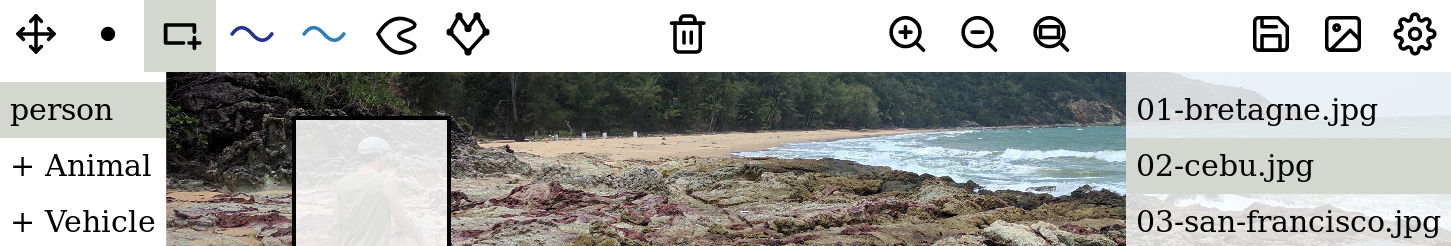
\includegraphics[width=\textwidth]{assets/img/annotation-app-thin.jpg}
  \caption{Screenshot of the interface of our image annotation Web application.}%
  \label{fig:teaser}
\end{figure}

Image annotations are required in a wide range of applications
including image classification (which requires textual labels),
object detection (bounding boxes), or image segmentation (pixel-wise classification).
The rise and successes of deep learning lead to an increasing need for annotations,
as training sets should be of a large size for these algorithms to be efficient.
Yet, researchers still spend time and resources
to create ad hoc tools to prepare those datasets.
The application we present in this chapter aims at providing a customizable tool
to fulfill most image annotation needs.

\begin{table*}[ht]
\centering
\begin{tabular}{lcl}
Application
	& Year
    & Tools\\
    \midrule
LabelMe
	& 2008
	& bbox, polygon, iterative semi-automatic segmentation\\
VIA
	& 2016
	& bbox, polygon, point, circle, ellipse\\
Labelbox
	& 2018
	& bbox, polygon, point, line\\
Dataturks
	& 2018
    & bbox, polygon\\
Ours
	& 2018
	& bbox, polygon, point, stroke, outline\\
\end{tabular}

\caption{Most relevant image annotation Web applications (tools).}%
\label{tab:web-apps-1}
\end{table*}

\begin{table*}[ht]
\centering
\begin{tabular}{lllll}
Application
    & \makecell[l]{Configurable\\interface}
    & \makecell[l]{Tasks\\management}
    & Type
    & License \\
    \midrule
LabelMe
    & no
    & Mturk integration
    & server
    & OSS \\
VIA
    & no
    & no
    & client
    & OSS \\
Labelbox
    & yes
    & yes
    & server
    & private \\
Dataturks
    & no
    & yes
    & server
    & private \\
Ours
    & yes
    & Mturk integration
    & client
    & OSS \\
\end{tabular}
\caption{Most relevant image annotation Web applications (application type).}%
\label{tab:web-apps-2}
\end{table*}

% \begin{figure*}[ht]
%     \centering
%     \begin{subfigure}[b]{0.575\textwidth}
%         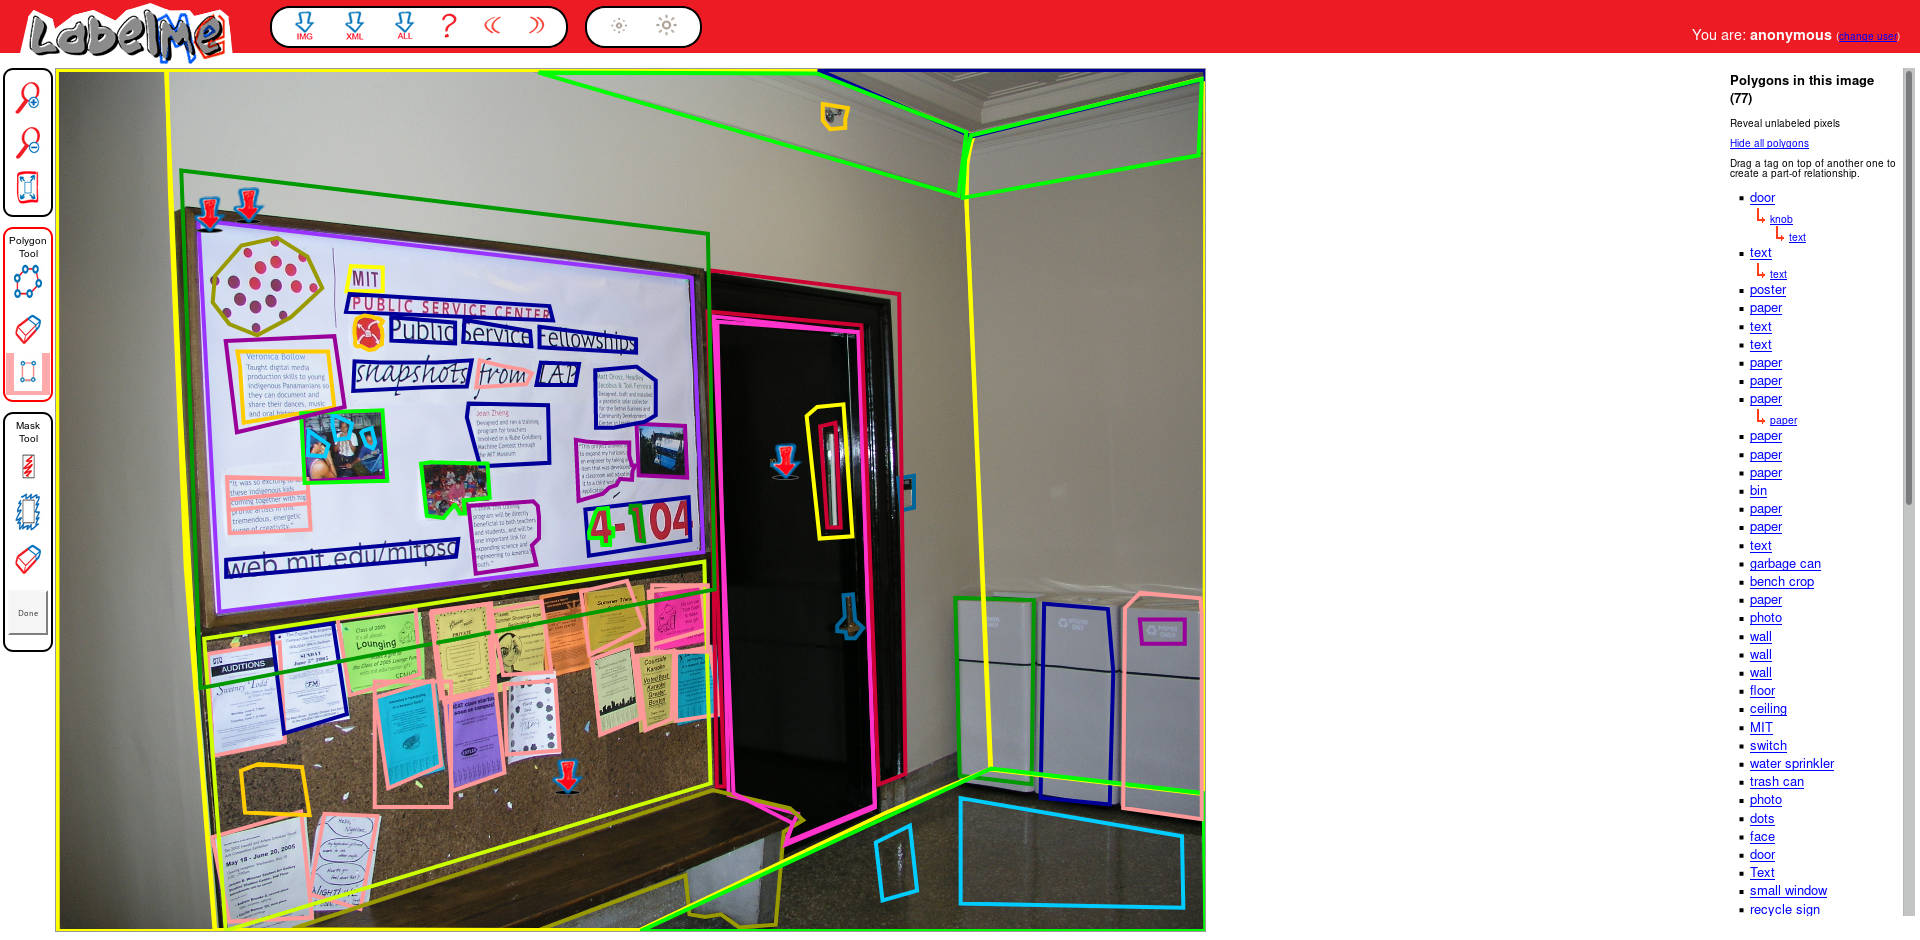
\includegraphics[width=\textwidth]{assets/img/labelme.jpg}
%         \caption{LabelMe}
%     \end{subfigure}
%     \hfill
%     \begin{subfigure}[b]{0.405\textwidth}
%         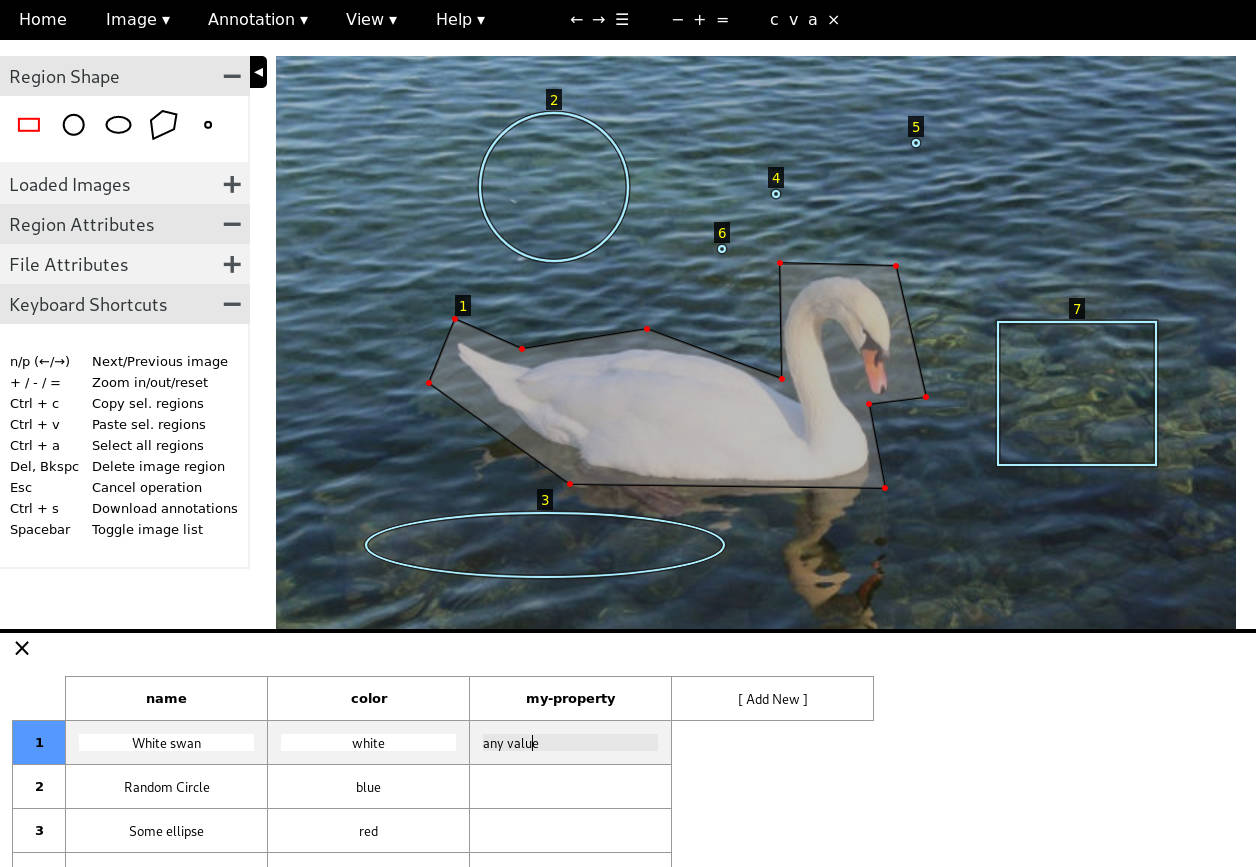
\includegraphics[width=\textwidth]{assets/img/via.jpg}
%         \caption{VIA}
%     \end{subfigure}
%     \hfill
%     \begin{subfigure}[b]{0.42\textwidth}
%         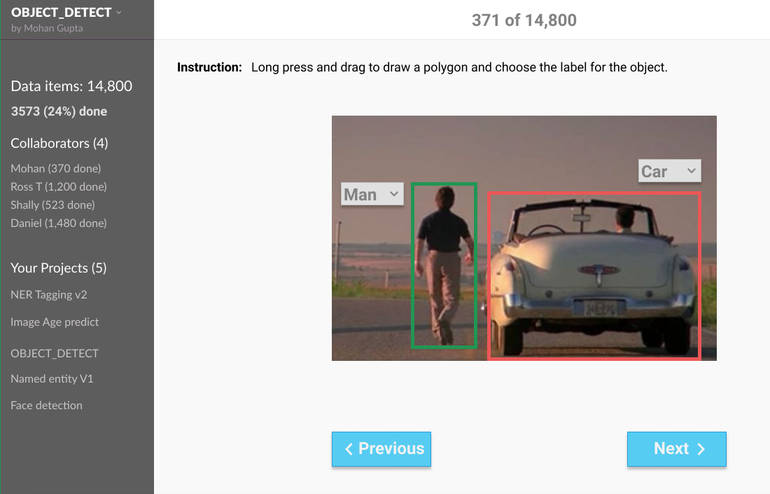
\includegraphics[width=\textwidth]{assets/img/dataturks.jpg}
%         \caption{Dataturks}
%     \end{subfigure}
%     \hfill
%     \begin{subfigure}[b]{0.56\textwidth}
%         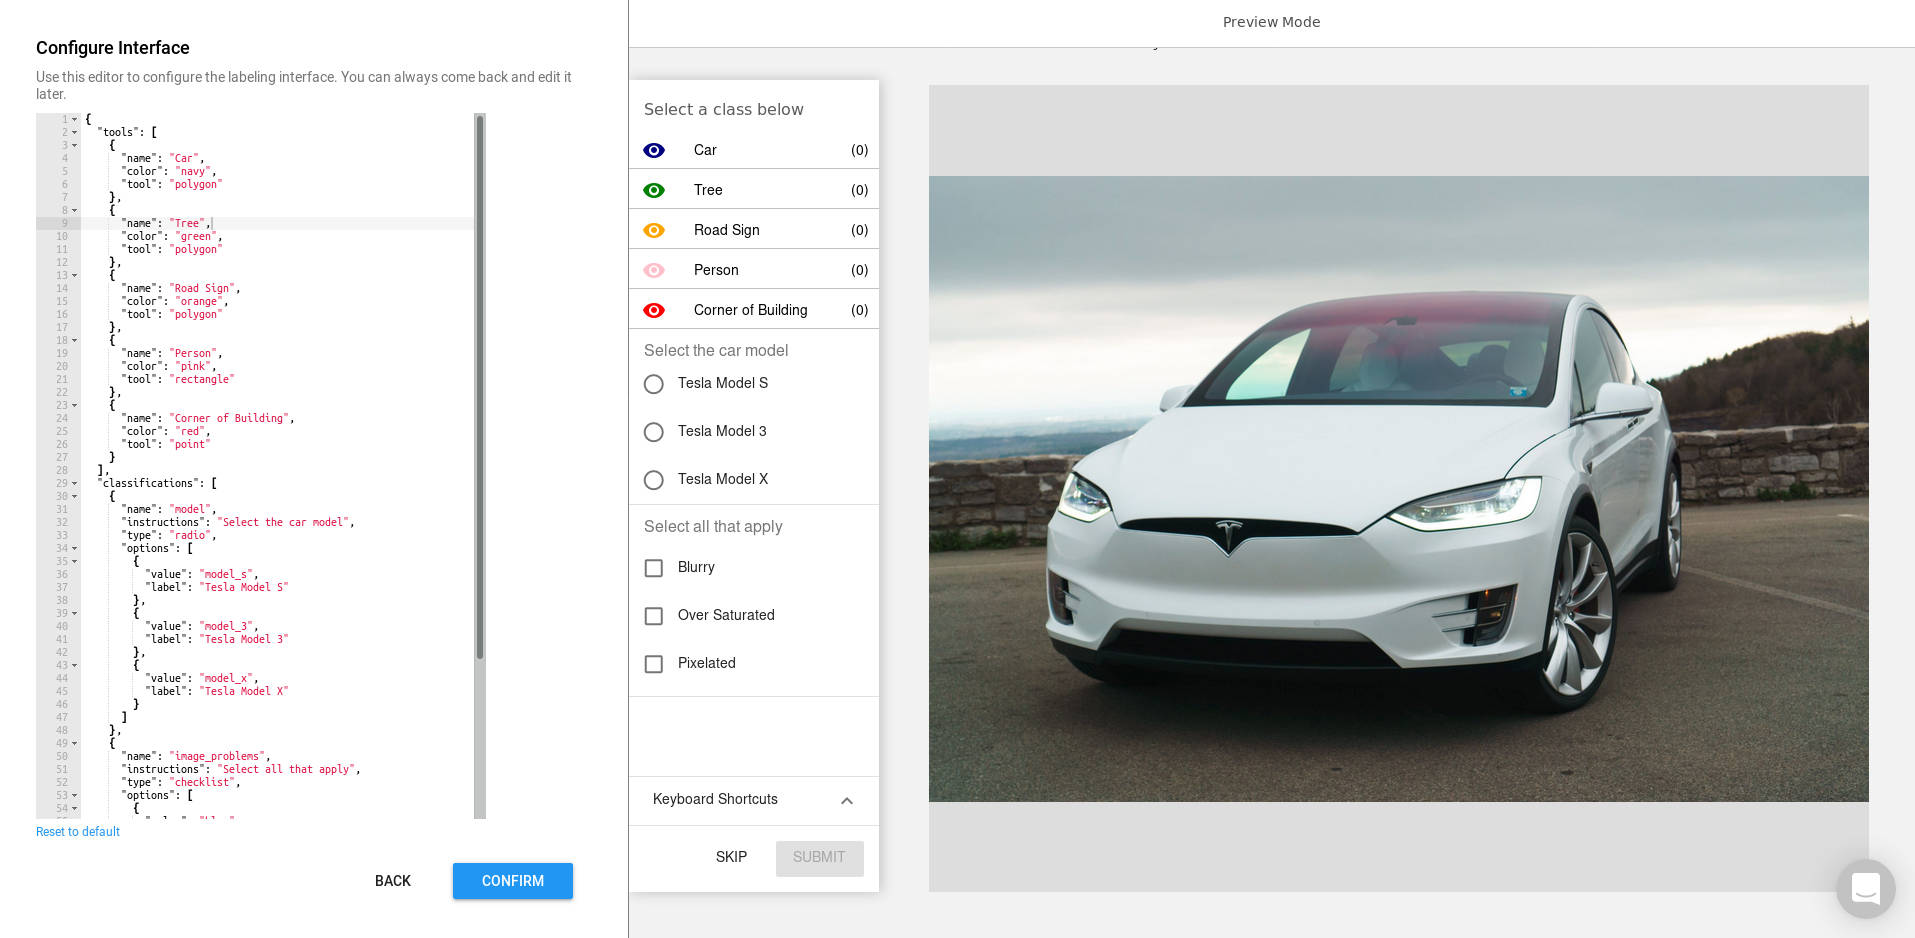
\includegraphics[width=\textwidth]{assets/img/label-box-config.jpg}
%         \caption{Labelbox}
%     \end{subfigure}
%     \caption{Interfaces of main other Web annotation applications}\label{fig:interfaces}
% \end{figure*}

Many image annotation applications already exist (Table~\ref{tab:web-apps-1}).
LabelMe~\cite{russell2008labelme}, one of the most popular,
provides an interface for drawing bounding boxes and polygons
around objects in an image.
It has been used extensively to create datasets for image segmentation.
Some more recent softwares share the same goals, with their own specificities.
For example, Labelbox~\cite{labelbox} and
Dataturks~\cite{dataturks} provide annotation tasks management,
particularly useful when crowdsourcing the annotations;
these softwares are proprietary.
The VGG Image Annotator (VIA~\cite{dutta2016via})
is an open-source client application like ours,
with the specificity of providing annotation attributes,
editable in a spreadsheet format.

We release an open-source application~\cite{annotationappgithub},
entirely client side, meaning that no data is uploaded to any server.
Images are loaded from files and annotated locally, in the browser.
The simplest tool, from a user perspective, should be immediately available
i.e.\ should not require any additional installation to be fully functional.
Our image annotation software is thus a Web-based application,
easily configurable to fit users needs, as well as
embeddable in the Mechanical Turk platform to design crowdsourcing campaigns.

We first present the features of our application, then describe its architecture.
Finally, we explain how it can be used to start crowdsourcing experiments.


\section{Presentation of the application}

A screenshot of the application can be seen in Figure~\ref{fig:teaser}.
The image to be annotated occupies the central part of the screen;
a toolbar is located on top, object classes are available on the left
and images to be annotated on the right.


\textbf{Images}.
Multiple images can be loaded at the same time using the image icon
on the top-right corner of the application.
These images are not uploaded on the server,
and can either be loaded locally from the client's machine,
or from a distant server.
% * <matthieu.pizenberg@gmail.com> 2018-05-20T06:53:31.040Z:
% 
% > or from a distant server.
% Seulement quand c'est fait directement dans le champ images des "flags" au démarrage de l'appli, pas en cliquant sur le bouton
% 
% ^ <matthieu.pizenberg@gmail.com> 2018-05-20T09:57:23.955Z.


\textbf{Tools}.
Our application includes several tools to annotate images.
Icons for these tools are depicted in Figure~\ref{fig:icons}.
From left to right, the first available annotation is the point,
that can be useful to designate objects in the image.
It can also be used as a seed in region-growing image segmentation methods.
The second annotation we included is the bounding box,
which provides the localization of objects in the image,
and is used in object detection problems.
The information we acquire are the left, right, top and bottom coordinates
of the bounding box.
The third annotation we chose to implement is the stroke,
or scribble, which is a popular interaction in image segmentation.
It consists in a sequence of points, interpreted as a continuous line.
The outline, fourth type of annotation,
is a closed shape, typically drawn around objects.
It is comparable to a bounding box in essence,
but provides a more precise location of objects.
Finally, polygons can also be drawn (as in LabelMe, for instance),
by successively clicking new points as vertices.


All these tools are available both with a mouse or a touch interaction.
As a matter of fact, some tools are better suited to touch devices
(for example, outlines) than others (polygons).

\begin{figure}[ht]
\centering

\includegraphics[width=0.8\columnwidth]{assets/img/annotation-tools.png}
\caption{Annotation tools icons}%
\label{fig:icons}
\end{figure}


\textbf{Object classes}.
For most annotation tasks, we also need to differentiate objects in the images.
Typically each annotated area is attributed a class, or label.
The PASCAL VOC dataset~\cite{everingham2010pascal}, for example,
is composed of 20 classes, grouped by categories:
\begin{itemize}
\item \textit{Person}: person
\item \textit{Animal}: bird, cat, cow, dog, horse, sheep
\item \textit{Vehicle}: aeroplane, bicycle, boat, bus, car, motorbike, train
\item \textit{Indoor}: bottle, chair, dining table, potted plant, sofa, tv/monitor
\end{itemize}

In our application, classes are specified in a JSON configuration file.
A strict corresponding config for PASCAL VOC classes
is presented in Listing~\ref{lst:pascal}.

\lstinputlisting[language=json,caption={A configuration file to annotate the PASCAL dataset.},float,label={lst:pascal}]{assets/code/config-pascal.json}

To attribute a class to an annotation,
a user should first select the class in the left sidebar,
then use a tool to create an annotation.
Selecting a class in the left sidebar also highlights the annotations
corresponding to this class.


\textbf{Configuration file}.
The five annotation tools are optionally made available by the configuration file.
In Listing~\ref{lst:pascal}, the last line of the depicted configuration file
contains an \texttt{annotations} field, listing the tools that should be available.
In this case, they all are.

In addition to the five fundamental annotation types,
each type can be derived in virtually any number of variations.
For example, interactive segmentation algorithms often require
\textit{foreground} and \textit{background} scribbles.
In our application, this would mean the user would need to draw two types of strokes.
This can be achieved using the configuration file,
as in Listing~\ref{lst:variations}.
Such configuration would result in two stroke icons in the toolbar,
of different colors, just as in Figure~\ref{fig:teaser}.

\lstinputlisting[language=json,caption={A configuration file to include two types of strokes.},float,label={lst:variations}]{assets/code/config-variations.json}


\section{Technical choices}

The application code is organized in two parts:

\begin{itemize}
\item A minimalist Node.js server, located in the \verb|server/| directory.
	It is statically serving the content of \verb|server/dist/|
    with compression.
\item A complete Elm client application, located in the \verb|client/| directory.
    It follows the Elm architecture presented in the previous chapter.
    We present the model, messages, and specific views of this application in this section.
    The compiled application weighs 150 kB gzipped,
    which is great for low bandwidth connections.
\end{itemize}


\subsection{The model states}

The \verb|state| is the main component of the \verb|Model|.
It contains the images and configuration loaded as well as the annotations performed.
Its type is defined as in Listing~\ref{lst:state}
and can be modeled as a finite state machine, visualized in Figure~\ref{fig:states}.

\lstinputlisting[language=elm,caption={State type definition.},label={lst:state},float]{assets/code/State.elm}

\begin{figure}[ht]
\centering
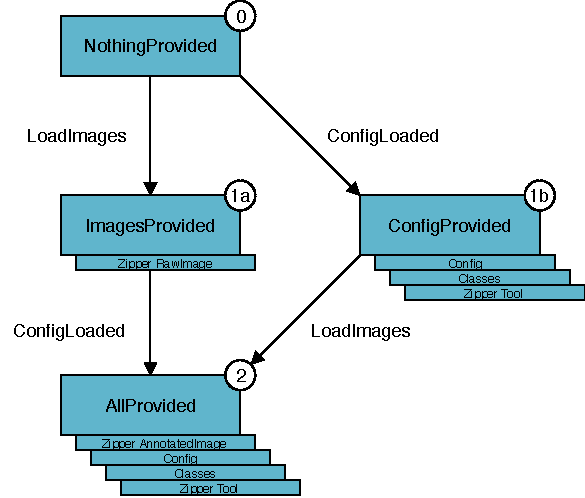
\includegraphics[width=\columnwidth]{assets/img/states-draw-io.pdf}
\caption{The application states.}%
\label{fig:states}
\end{figure}

The application available online starts in state 0 (\verb|NothingProvided|)
and enables you to reach state 2 (\verb|AllProvided|)
with buttons to load images and configuration.
Two messages called \verb|LoadImages| and \verb|ConfigLoaded| produce
transitions in the state machine.


\subsection{The messages}

All modifications of the model are understood
by looking at the \verb|Msg| type definition (Listing~\ref{lst:msg}).
The \verb|update| function then performs the modifications described by those messages.

\lstinputlisting[language=elm,caption={Msg type definition.},label={lst:msg},float]{assets/code/Msg.elm}

\begin{itemize}
\item The \verb|WindowResizes| message is triggered when the application is resized.
	In the update function, it takes the new size and recomputes some view parameters.
\item A \verb|PointerMsg| message is triggered by pointer events (mouse, touch, etc.).
	In the update function, this is the message activating
	all the annotations logic code of our application.
\item The messages \verb|SelectImage|, \verb|SelectTool| and \verb|SelectClass|
	are generated when clicking on images, tools and classes.
\item Files are handled by five messages:
	\begin{itemize}
	\item When loading images from the file explorer,
		a \verb|LoadImages| message is generated with a list of the images files
		and their names as identifiers.
		For each image correctly loaded an \verb|ImageLoaded| message is generated,
		providing a local url, corresponding to the image in memory.
    \item The messages \verb|LoadConfig| and \verb|ConfigLoaded| behave similarly.
    \item The \verb|Export| message causes the application to serialize into JSON
		all the annotations, and asks the user to save the generated file.
		It is triggered by clicking on the export button of the top action bar.
	\end{itemize}
\item Whenever an event should change the zooming level of the drawing area,
	a \verb|ZoomMsg| message is  generated.
\item Finally, the \verb|RemoveLatestAnnotation| message is also explicit.
\end{itemize}


\subsection{The view}

The view of this application is based on four components,
each implemented in its own module, with potentially different versions
depending on the current state of the application.
\begin{itemize}
\item The top action bar (\verb|src/View/ActionBar.elm|).
\item The center annotations viewer area\\(\verb|src/View/AnnotationsArea.elm|).
\item The right images sidebar\\(\verb|src/View/DatasetSideBar.elm|).
\item The left classes sidebar\\(\verb|src/View/ClassesSideBar.elm|).
\end{itemize}


% \subsection{Startup and interactions with JavaScript}

% Compiling the Elm application code produces a JavaScript file \verb|Main.js|.
% This file has to be embeded in an html document.
% Then the application is started with parameters called "flags"
% as demonstrated in Listing~\ref{lst:start}.

% \lstinputlisting[language=javascript,caption={JavaScript code to embed the Elm application.},label={lst:start},float]{assets/code/start.js}


\subsection{Library and application duality}

In order to offer a turnkey solution to image annotations,
we created a configurable application solving most needs.
But we also thought of cases where advanced modifications are required.
Consequently, the foundation of this application has been extracted
in the independent package elm-image-annotation~\cite{annotationpackage}.
It is designed as an API to create, modify and visualize geometric shapes,
useful in the context of image annotation.

Modules for manipulation and serialization (in JSON) of annotations are
under the \verb|Annotation.Geometry| namespace.
It already contains one module for each tool presented earlier.
If you want to introduce a new tool, this is where you can create a new module.

This package also contains the following important modules,
under the \verb|Annotation| namespace:
\begin{itemize}
	\item \verb|Annotation.Style|:
		defines types describing appearance of points, lines and fillings of annotations.
	\item \verb|Annotation.Svg|:
		exposes functions rendering SVG elements for each annotation kind.
	\item \verb|Annotation.Viewer|:
		manages the central visualization area,
		supporting zooming and translations, relative to an image frame.
\end{itemize}
If you are interested in creating another rendering target than SVG,
like canvas or WebGL, it would require alternative modules
to \verb|Annotation.Svg| and \verb|Annotation.Viewer|.
The rest of the code can stay unchanged.


\section{Crowdsourcing annotations}

Image annotation interfaces are often used in the context
of large datasets of images to annotate.
As such, tasks management for crowdsourcing campaigns is an important feature. 
Labelbox and Dataturks are all-in-one services providing
tasks management directly in their applications.
Just like LabelMe, we choose instead to provide a configuration,
ready to use with Amazon Mechanical Turk (Mturk).

Mturk comes in two sides. A ``requester'' is defining a set of tasks
while a ``worker'' is performing them.
Workers are payed by requesters through the Mturk service.
The concept of a ``HIT'' (Human Intelligence Task) characterizes the task unit.
In our case, one HIT means one image to be annotated.
We describe in details how to setup a campaign with our template
in the application documentation.


\section{Acknowledgments}

We would like to thank:

\begin{itemize}
	\item @tforgione and @GarciaDelMolino for your wise feedbacks.
	\item @dncg for your Windows tests.
	\item The online Elm community for their help along the road:
		@evancz for the delightful Elm language,
		@ianmackenzie for your fantastic geometry library,
		@mdgriffith for your very refreshing layout library,
		@luke for the amazing tool Ellie,
		@norpan, @jessta, @loganmac, @antew, for your invaluable help on slack.
\end{itemize}


\section{Conclusion}

In this chapter we have introduced our Web-based image annotation application.
More information is available in the online documentation~\cite{annotationappdoc}.
Evolutions of this application are still developed in alternative branches to keep
the master branch in a stable state. We welcome all forms of feedback and contribution.

\alert{Mention usage of this application in a crowdsourcing campaign
to annotate pascal voc. Add transition to next part of the thesis.}



\part{RGB-D Visual Odometry}%
\label{prt:rgb_d_vo}
This part is about RGB-D visual odometry.
Introduction and motivation/justification.

\begin{itemize}
	\item Lightweight
	\item Smartphones
	\item Depth sensors
	\item Augmented reality
\end{itemize}

\chapter{Introduction to the RGB-D Visual Odometry Problem}%
\label{cha:rgbd_vo}

\minitoc%
\clearpage

\section{Image Formation (copied)}%
\label{sec:image-formation}

\alert{Copied from cremers mvg, need reformulation}

\subsection{Historic Remarks}%
\label{sub:historic_remarks}


\begin{figure}[h]
\centering
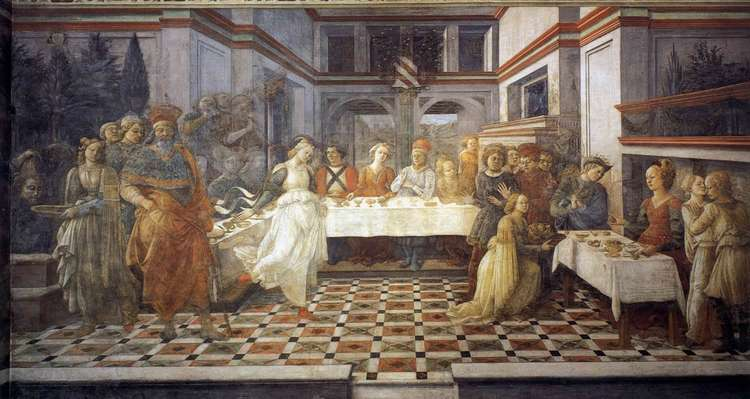
\includegraphics[width=0.5\columnwidth]{assets/img/lippi_feast_herod.jpg}
\caption{Filippo Lippi, ``The Feast of Herod: Salome's Dance.''
Fresco, Cappella Maggiore, Duomo, Prato, Italy, c.1460--1464.}%
\label{fig:lippi_feast_herod}
\end{figure}

\begin{figure}[h]
\centering
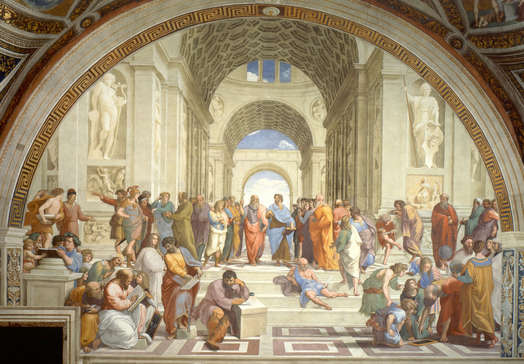
\includegraphics[width=0.5\columnwidth]{assets/img/raphael_school_athens.jpg}
\caption{Raphael, The School of Athens (1509)}%
\label{fig:raphael_school_athens}
\end{figure}

\begin{figure}[h]
\centering
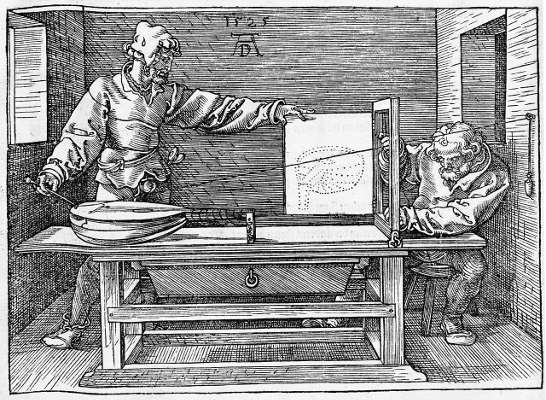
\includegraphics[width=0.5\columnwidth]{assets/img/durer_perspective_machine.jpg}
\caption{D\"urer's perspective machine (1525)}%
\label{fig:durer_perspective_machine}
\end{figure}

The study of the image formation process has a long history.
The earliest formulations of the geometry of image formation
can be traced back to \textbf{Euclid} (4th century B.C.).
Examples of a partially correct \textbf{perspective projection}
are visible in the \textbf{frescoes and mosaics of Pompeii} (1 B.C.).\\

These skills seem to have been lost with the fall of the Roman empire.
Correct perspective projection emerged again around 1000 years later
in early \textbf{Renaissance art}.\\

Among the proponents of perspective projection are the
Renaissance artists \textbf{Brunelleschi, Donatello} and \textbf{Alberti}.
The first treatise on the projection process, \textbf{``Della Pittura''},
was published by \textbf{Leon Battista Alberti}.\\

Appart from the geometry of image formation, the study of the
interaction of light with matter was propagated by artists like
\textbf{Leonardo da Vinci} in the 1500s and by Renaissance painters
such as \textbf{Caravaggio} and \textbf{Raphael}.\\

In Figure~\ref{fig:lippi_feast_herod} and Figure~\ref{fig:raphael_school_athens}
the perspective emerges from the vanishing point.

\begin{figure}[h]
\centering
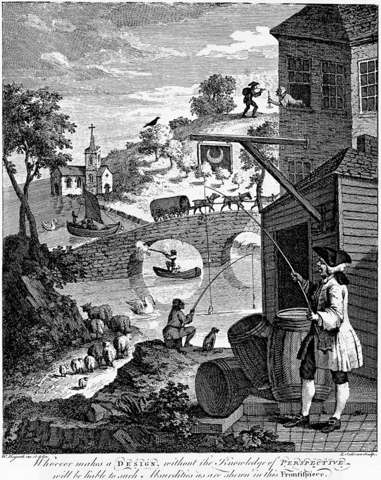
\includegraphics[width=0.5\columnwidth]{assets/img/hogarth_satire.jpg}
\caption{Satire by Hogarth 1753}%
\label{fig:hogarth_satire}
\end{figure}

\begin{figure}[h]
\centering
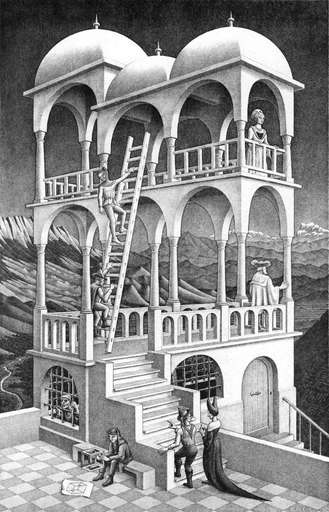
\includegraphics[width=0.5\columnwidth]{assets/img/escher_belvedere.jpg}
\caption{Escher, Belvedere 1958}%
\label{fig:escher_belvedere}
\end{figure}

D\"urer devised a machine to get a perspectively correct image,
see Figure~\ref{fig:durer_perspective_machine}.
It is a manual reproduction of what a camera does today.\\

Many artists played with those perspective rules to create images
that seems locally correct but have inconsitent depth or gravity, like
in Figures~[\ref{fig:hogarth_satire},\ref{fig:escher_belvedere}].


\subsection{Mathematical Representation}%
\label{sub:mathematical_representation}


\begin{figure}[h]
\centering
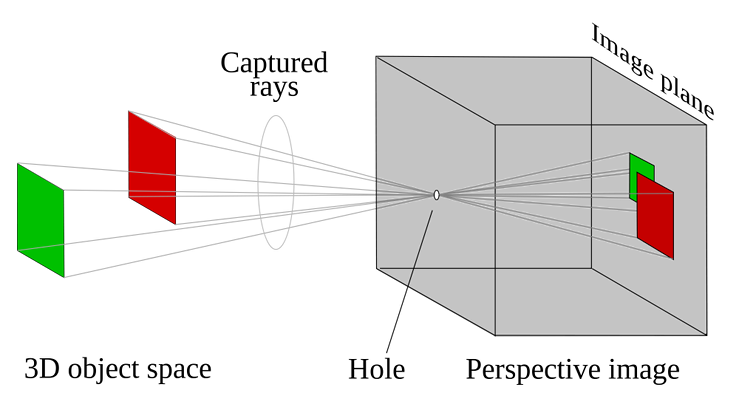
\includegraphics[width=0.5\columnwidth]{assets/img/pinhole_camera.png}
\caption{Pinhole camera model}%
\label{fig:pinhole_camera}
\end{figure}

\begin{figure}[h]
\centering
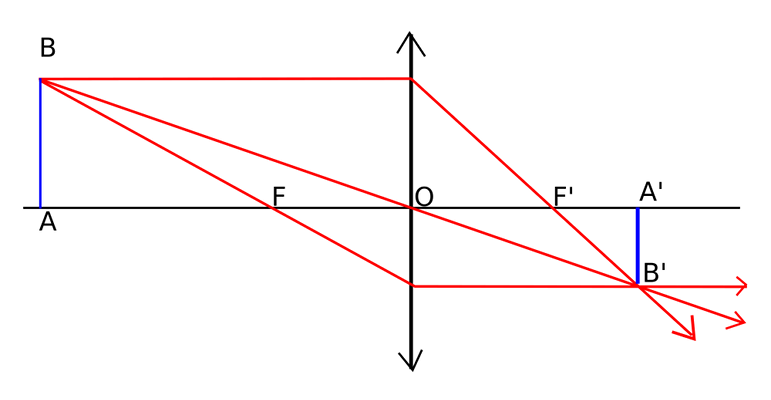
\includegraphics[width=0.5\columnwidth]{assets/img/convex_lense.png}
\caption{Thin convex lense model}%
\label{fig:convex_lense}
\end{figure}

Perspective projection emerges by the so-called pinhole camera model
(see Figure~\ref{fig:pinhole_camera}).
It's main issue is that the hole has to be very small,
perventing light to enter the capture device.
In order to augment the the amount of light we use lenses\\

As visible in (Figure~\ref{fig:convex_lense}), the image is upside down
in the image plan. In order to avoid dealing with minus signs in the
equations, we pretend that the image plan is virtually on the same
side than the object. The perspective thansformation $\pi$ is given by
\[ \pi : \R^3 \rightarrow \R^2; \quad
	\bm{X} \mapsto x = \pi(\bm{X}) =
	\begin{pmatrix}
		f \frac{X}{Z} \\
		f \frac{Y}{Z} \\
	\end{pmatrix}
\]
Where $f$ is the focal length, $X,Y,Z$ are the object coordinates
in the 3D world, the $z$ axis being the camera axis.
The one challenge we have to overcome, is that this transformation is non linear.\\

In order to do so, we will use \textbf{homogeneous coordinates},
which is basically similar to multiplying everything by $Z$:
\[ Z \bm{x} = Z \begin{pmatrix} x \\ y \\ 1 \end{pmatrix} =
	\begin{pmatrix}
		f & 0 & 0 & 0 \\
		0 & f & 0 & 0 \\
		0 & 0 & 1 & 0 \\
	\end{pmatrix}
	\begin{pmatrix}
		X \\ Y \\ Z \\ 1
	\end{pmatrix}
	= K_f \Pi_0 \bm{X}
\]
Where we have introduced the two matrices
\[K_f \equiv
	\begin{pmatrix}
		f & 0 & 0 \\
		0 & f & 0 \\
		0 & 0 & 1 \\
	\end{pmatrix}
	\quad \text{and} \quad
	\Pi_0 \equiv
	\begin{pmatrix}
		1 & 0 & 0 & 0 \\
		0 & 1 & 0 & 0 \\
		0 & 0 & 1 & 0 \\
	\end{pmatrix}
\]
The matrix $\Pi_0$ is referred to as the \textbf{standard projection matrix}.
A first order approximation can consider that all object points
are approximately at the same distance $\lambda > 0$. Thus we obtain:
\[\lambda \bm{x} = K_f \Pi_0 \bm{X}\]

We know that due to the \textbf{rigid motion of the camera},
the point $\bm{x}$ \textbf{in camera coordinates} is given as a function
of the point in \textbf{wold coordinates} $\bm{X}_0$ by:
\[\bm{X} = R \bm{X}_0 + T\]
or in homogeneous coordinates:
\[\bm{X} = g \bm{X}_0 = \begin{pmatrix}R & T \\ 0 & 1\end{pmatrix} \bm{X}_0\]
In total, the transformation from world coordinates to image coordinates
is therefore given by:
\[\boxed{\lambda\ \bm{x} = K_f\ \Pi_0\ g\ \bm{X}_0}\]


\subsection{Intrinsic Parameters}%
\label{sub:intrinsic_parameters}


If the camera is not centered at the optical center, we have an additional
translation $o_x, o_y$. The point were the optical axis intersects
the image plan is called the \textbf{principal point}.\\

If pixels do not have unit scale, we need to introduce
additional scaling factors $s_x$ and $s_y$.
If pixels are not rectangular, we also have a \textbf{skew factor} $s_{\theta}$.\\

The transformation from initial real world coordinates to final pixel coordinates
follows the following steps:
World (3D, $\bm{X}_0$) $\mapsto$ Camera (3D, $\bm{X}$)
$\mapsto$ Image (2D, $\bm{x}$) $\mapsto$ Pixel (2D, $\bm{x'}$).\\

The pixel coordinates $\bm{x'} = (x',y',1)$ are given by:
\[\lambda \begin{pmatrix}x' \\ y' \\ 1\end{pmatrix} =
	K_s\ K_f\ \Pi_0
	\begin{pmatrix}X \\ Y \\ Z \\ 1\end{pmatrix}
\]
where
\[K_s = \begin{pmatrix}
		s_x & s_{\theta} & o_x \\
		0 & s_y & o_y \\
		0 & 0 & 1 \\
	\end{pmatrix}
	\quad K_f =
	\begin{pmatrix}
		f & 0 & 0 \\
		0 & f & 0 \\
		0 & 0 & 1 \\
	\end{pmatrix}
\]
We call $K = K_s\ K_f$ the \textbf{intrinsic parameter matrix}.\\

Therefore, as a function of world coordinates, we have:
\[\boxed{ \lambda\ \bm{x'} = \Pi\ \bm{X}_0
	= K\ \Pi_0\ g\ \bm{X}_0}
\]
The $3 \times 4$ matrix $\Pi$ is called a \textbf{general projection matrix}.
If we get rid of $\lambda$ we obtain the following coordinates:
\[ x' = \frac{\tr{\pi_1} \bm{X}_0}{\tr{\pi_3} \bm{X}_0},\quad
 y' = \frac{\tr{\pi_2} \bm{X}_0}{\tr{\pi_3} \bm{X}_0},\quad
 z' = 1
\]
where $\tr{\pi_1}, \tr{\pi_2}, \tr{\pi_3} \in \R^4$
are the three rows of the projection matrix $\Pi$.


\subsection{Radial Distortion}%
\label{sub:radial_distortion}


\begin{figure}[h]
\centering
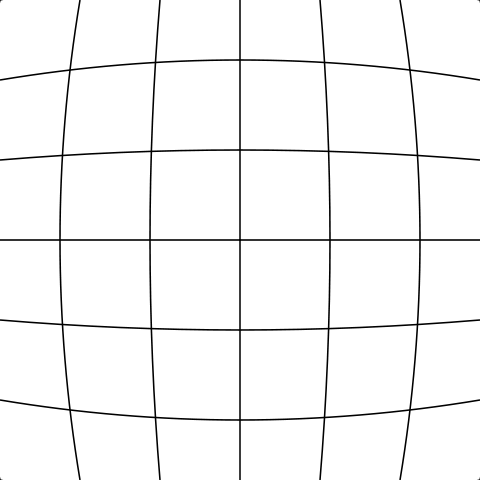
\includegraphics[width=0.5\columnwidth]{assets/img/barrel_distortion.png}
\caption{Grid projection with radial distortion.}%
\label{fig:radial_distortion}
\end{figure}

The intrinsic parameters in the matrix $K$ model linear distortions
in the transformation to pixel coordinates.
In practice however, one can also encounter significant
\textbf{distortions along the radial axis}~[\ref{fig:radial_distortion}],
in particular in a wide field of view is used or if one uses cheaper cameras
such as webcams.
A simple effective model for such distortions is:
\[
	x = x_d ( 1 + a_1 r^2 + a_2 r^4 ),
	y = y_d ( 1 + a_1 r^2 + a_2 r^4 )
\]
where $\bm{x} \equiv (x_d, y_d)$ is the distorted point,
$r^2 = \|\bm{x}\|^2$.
Usually, $a_1$ and $a_2$ are estimated through a calibration step.\\

Other more sophisticated models exist (Devernay and Faugeras '95).
Parameters are computed from
\textbf{distortions of straight lines} (see Figure~\ref{fig:radial_distortion})
or \textbf{simultaneously with the 3D reconstruction}
(Zhang '96, Stein '97, Fitzgibbon '01).


\subsection{Projective Geometry}%
\label{sub:projective_geometry}


In order to formally write transformations by linear operations,
we made extensive use of \textbf{homogeneous coordinates} to represent
3D point as a 4D-vector $(X,Y,Z,1)$ with the last coordinate fixed to 1.
This normalization is not always necessary. One can represent 3D points
by a general 4D vector:
\[
	\bm{X} = (XW, YW, ZW, W)\ \in\ \R^4
\]
In general, an \textbf{n-dimensional projective space} $\mathbb{P}^n$
is the set of all one-dimensional subspaces (i.e.\ lines through the origin)
of the vector space $\R^{n+1}$.
A point $p \in \mathbb{P}^n$ can then be assigned homogeneous coordinates
$\bm{X} = \tr{(x_1, \ldots, x_{n+1})}$, among which at least one $x$ is nonzero.
For any nonzero $\lambda \in \R$, the coordinates
$\bm{Y} = \tr{(\lambda x_1, \ldots, \lambda x_{n+1})}$
represent the same point $p$.

\section{Representing a Moving Scene (copied)}%
\label{sec:moving-scene}

\alert{Copied from cremers mvg, need reformulation}

\subsection{The Origins of 3D Reconstruction}%
\label{sub:the_origins_of_3d_reconstruction}

The goal to reconstruct the three-dimensional structure of the world from
a set of two-dimensional views has long history in computer vision.
It is a classical \textbf{ill-posed problem}, because the reconstruction
consistent with a given set of observations/images is typically not unique.
Therefore, one will need to impose additional assumptions.
Mathematically, the study of geometric relations between a 3D scene
and the observed 2D projections is based on two types of transformations, namely:
\begin{itemize}
	\item \textbf{Euclidean motion} or \textbf{rigid body motion}
		representing the motion of the camera from one frame to the next.
	\item \textbf{Perspective projection} to account for the image formation
		process (see pinhole camera, etc).
\end{itemize}

The notion of perspective projection has its roots among the ancient Greeks
(Euclid of Alexandria, \roughly{} 400 B.C.) and the Renaissance period
(Brunelleschi \& Alberti, 1435).
The study of perspective projection lead to the field of
\textbf{projective geometry} (Girard Desargues 1648, Gaspard Monge 18th cent).\\

The first work on the problem of multiple view geometry was that of
\textbf{Erwin Kruppa (1913)} who showed that two views of five points
are sufficient to determine both the relative tansformation
(\textbf{motion}) between the two views and the 3D location (\textbf{structure})
of the points up to finitely many solutions.\\

A linear algorithm to recover structure and motion from two views based
on the epipolar constraint was proposed by \textbf{Longuet-Higgins}
in \textbf{1981}. An entire series of works along these lines was summarized
in several text books (Faugeras 1993, Kanatani 1993,
Maybank 1993, Weng et al. 1993).\\

Extensions to three views were developed by Spetsakis and Aloimonos '87, '90
, and by Shashua '94 and Hartley '95.
Factorization techniques for multiple views and orthogonal projection were
developed by Tomasi and Kanade 1992.\\

Depending on communities, the joint estimation of camera motion and 3D location is called
\textbf{structure and motion} or \textbf{visual SLAM}.

\subsection{3D Space \& Rigid Body Motion}%
\label{sub:3d_space_rigid_body_motion}


\subsubsection{Three-dimensional Euclidean Space}%
\label{ssub:three_dimensional_euclidean_space}

The three-dimensional Euclidean space $\E^3$ consists of all points
$p \in \E^3$ characterized by coordinates
	\[\bm{X} \equiv \tr{(X_1, X_2, X_3)} \in \R^3\]

such that $\E^3$ can be identified with $\R^3$.
That means we talk about points ($\E^3$) and coordinates ($\R^3$)
as if they were the same thing. Given two points $\bm{X}$ and $\bm{Y}$,
one can define a \textbf{bound vector} as
	\[v = \bm{Y} - \bm{X} \in \R^3\]

Considering this vector independent of its base point $\bm{Y}$ makes
it a \textbf{free vector}. The set of free vectors $v \in \R^3$
forms a linear vector space. By identifying $\E^3$ and $\R^3$,
one can endow $\E^3$ with a scalar product, a norm and a metric.
This allows to compute \textbf{distances, curve length, areas or volumes.}
\[\text{For a curve } \gamma : [0,1] \rightarrow \R^3,\quad
	l(\gamma) \equiv \int_{0}^1 | \dot{\gamma}(s) | d\!s\]


\subsubsection{Cross Product \& Skew-symmetric Matrices}%
\label{ssub:cross_product_and_skew_symmetric_matrices}

On $\R^3$ one can define a cross product
\[\times : \R^3 \times \R^3 \rightarrow \R^3,\quad u \times v =
	\begin{pmatrix}
		u_2v_3 - u_3v_2 \\
		u_3v_1 - u_1v_3 \\
		u_1v_2 - u_2v_1
	\end{pmatrix} \in \R^3\]

which is a vector \textbf{orthogonal to $u$ and $v$}.
Since $u \times v = -v \times u$, the cross product introduces an \textbf{orientation}.
Fixing $u$ induces a linear mapping $v \mapsto u \times v$ wich
can be represented by the \textbf{skew-symmetric matrix}
\[\widehat{u} = \hatmat{u_1}{u_2}{u_3} \in \RR{3}{3}\]

In turn, every skew symmetric matrix $M = -\tr{M} \in \RR{3}{3}$
can be identified with a vector $u \in \R^3$.
The operator $\widehat{}$ defines an \textbf{isomorphism} between $\R^3$
and the space $so(3)$ of the $3 \times 3$ skew-symmetric matrices.
Its inverse is denoted by $\vee : so(3) \rightarrow \R^3$.


\subsubsection{Rigid-body Motion}%
\label{ssub:rigid_body_motion}

A \textbf{rigid-body motion} (or rigid-body transformation)
is a family of maps
\[g_t : \R^3 \rightarrow \R^3;\quad \bm{X} \mapsto g_t(\bm{X}),\quad t \in [0,T]\]

which preserve the norm and cross product of any two vectors:
\begin{itemize}
	\setlength\itemsep{-0.2em}
	\item $\forall v \in \R^3, \quad |g_t(v)| = |v|$
	\item $\forall u,v \in \R^3, \quad g_t(u) \times g_t(v) = g_t(u \times v)$
\end{itemize}

Since norm and scalar product are related by the \textbf{polarization identity}
\[\inner{u}{v} = \frac{1}{4}(|u+v|^2 - |u-v|^2)\]

one can also state that a rigid-body motion is a map which
preserves inner product and cross product.
As a consequence, rigid-body motions also preserves the \textbf{triple product}
\[\forall u, v, w \in \R^3, \quad
	\inner{g_t(u)}{g_t(v) \times g_t(w)} = \inner{u}{v \times w}\]

which means that they are volume-preserving.


\subsubsection{Representation of Rigid-body Motion}%
\label{ssub:representation_of_rigid_body_motion}

Let $g_t$ our rigid body motion. We are going to detail what this transformation
is doing to the initial frame of orthonormal oriented vecors
$e_1, e_2, e_3 \in \R^3$.
We note the transformed vectors $r_i = g_t(e_i)$.
Scalar and cross product of these vectors are preserved:
	\[\tr{r_i}r_j = \tr{g_t(e_i)}g_t(e_j) = \tr{e_i}e_j = \delta_{ij}, \quad
	r_1 \times r_2 = r_3\]

The first constraint amounts to the statement that the matrix
$R = (r_1, r_2, r_3)$ is an orthogonal matrix: $\bm{\tr{R}R=R\tr{R}=I}$,
whereas the second property implies that $\bm{\det(R) = +1}$.
In other words: $R$ is an element of the group
$SO(3) = \{R \in \RR{3}{3}\ |\ \tr{R}R=I,\ \det(R) = +1\}$.\\

The motion of the origin can be represented by a \textbf{translation}
$\bm{T \in R^3}$. Thus the rigid body motion $g_t$ can be written as:
	\[g_t(x) = Rx + T\]


\subsubsection{Exponential Coordinates of Rotation}%
\label{ssub:exponential_coordinates_of_rotation}

We will now derive a representation of an \textbf{infinitesimal rotation}.
To this end, we consider a family of rotation matrices $R(t)$
which continuously transform a point from its original location
$(R(0) = I)$ to a different one.
	\[\bm{X}_{\text{trans}}(t) = R(t)\bm{X}_{\text{orig}}, \quad
	\text{with } R(t) \in SO(3)\]

Since $\forall t,\ R(t)\tr{R(t)} = I$, we have:
	\[\frac{d}{dt}(R\tr{R}) = \dot{R}\tr{R} + R\tr{\dot{R}}= 0
	\implies \dot{R}\tr{R} = -\tr{( \dot{R}\tr{R} )}\]

Thus, $\dot{R}\tr{R}$ is a \textbf{skew-symmetric matrix}.
As shown in the section about the $\widehat{}$ operator, this implies that
there exists a vector $w(t) \in \R^3$ such that:
	\[\dot{R}(t)\tr{R}(t) = \widehat{w}(t)
	\Leftrightarrow \bm{ \dot{R}(t) = \widehat{w}(t)R(t)}\]

Since $R(0) = I$, it follows that $\dot{R}(0) = \widehat{w}(0)$.
Therefore, the \textbf{skew-symmetric matrix $\bm{\widehat{w}(0) \in so(3)}$
gives the first order approximation of a rotation:}
	\[R(dt) = R(0) + dR = I + \widehat{w}(0) dt\]


\subsection{The Lie Group $SO(3)$}%
\label{sub:the_lie_group_so_3_}


\subsubsection{Lie Group and Lie Algebra}%
\label{ssub:lie_group_and_lie_algebra}

The above calculations showed that the effect of any infinitesimal
rotation $R \in SO(3)$ can be approximated by an element from
the space of skew-symmetric matrices
	\[so(3) = \{ \widehat{w}\ |\ w \in \R^3\}\]

The rotation group $SO(3)$ is called a \textbf{Lie group}.
The space $so(3)$ is called its \textbf{Lie algebra}.\\

\underline{Definition:}
A \textbf{Lie group} (or infinitesimal group) is a smooth manifold that
is also a group, such that the group operations multiplication
and inversion are smooth maps.\\

As shown above: \textbf{The Lie algebra $\bm{so(3)}$ is the tangent space
at the identity of the rotation group $\bm{SO(3)}$.}\\

An \textbf{algebra over a field $\bm{K}$} is a vector space $V$ over $K$
with multiplication on the space $V$.
Elements $\widehat{w}$ and $\widehat{v}$ of the Lie algebra
generally do not commute.
One can define the \textbf{Lie bracket}
\[[\cdot,\cdot]: so(3) \times so(3) \rightarrow so(3);\quad
[\widehat{w},\widehat{v}] \equiv \widehat{w}\widehat{v} - \widehat{v}\widehat{w}\]


\subsubsection{Sophus Lie (1841--1899)}%
\label{ssub:sophus_lie_1841_1899_}

\begin{figure}[ht]
\centering
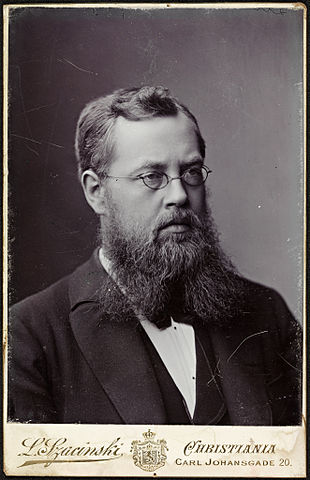
\includegraphics[width=10em]{assets/img/sophus_lie.jpg}
\caption*{Portrait of Marius Sophus Lie}
\end{figure}

Marius Sophus Lie was a Norwegian-born mathematician.
He created the theory of \textbf{continuous symmetry}, and applied it to
the study of geometry and differential equations. Among his greatest
achievements was the discovery that continuous transformation
groups are better understood in their linearized versions
(``Theory of transformation groups'' 1893).
These \textbf{infinitesimal generators} form a structure which is today
known as a \textbf{Lie algebra}. The linearized version of the group law
corresponds to an operation on the Lie algebra known as
the \textbf{commutator bracket} or \textbf{Lie bracket}.
1882 Professor in Christiania (Oslo),
1886 Leipzig (succeeding Felix Klein),
1898 Christiania.


\subsubsection{The Exponential Map}%
\label{ssub:the_exponential_map}

Given the infinitesimal formulation of rotation,
we got to the differential equation system:
	\[\left\{ \begin{aligned}
		\dot{R}(t) &= \widehat{w}(t)R(t) \\
		R(0) &= I \\
	\end{aligned}\right.\]

If we assume that $\widehat{w}(t)$ is constant in time ($=\widehat{w}$),
this known equation has the solution:
	\[R(t) = e^{\widehat{w}t}
		= \sum_{n=0}^{\infty} \frac{{(\widehat{w}t)}^n }{n!}
		= I + \widehat{w}t + \frac{{(\widehat{w}t)}^2 }{2!} + \ldots \]

which is a rotation around the axis $w \in \R^3$
by an angle of t (if $\|w\| = 1$). Alternatively, one can absorb
the scalar $t \in \R$ into the skew  symmetric matrix $\widehat{w}$
to obtain $R(t) = e^{\widehat{v}}$ with $\widehat{v} = \widehat{w}t$.
This \textbf{matrix exponential} therefore defines a map from
the Lie algebra to the Lie group:
	\[\exp : so(3) \rightarrow SO(3);\quad \widehat{w}\mapsto e^{\widehat{w}}\]


\subsubsection{The Logarithm of $SO(3)$}%
\label{ssub:the_logarithm_of_so_3_}

There is conversely a mapping from the Lie group to the Lie algebra.
For any rotation matrix $R \in SO(3)$, there exists a $w \in \R^3$
such that $R = \exp(\widehat{w})$. Such an element is denoted by
$\widehat{w} = \log(R)$. If $R \ne I$, we note $r_{ij}$ its coefficients
and $w$ is given by:
	\[\left\{ \begin{aligned}
		|w| &= \inv{\cos}\left(\frac{\text{trace}(R)-1}{2}\right)\\
		\frac{w}{|w|} &= \frac{1}{2\sin(|w|)}
			\begin{pmatrix}
				r_{32} - r_{23} \\
				r_{13} - r_{31} \\
				r_{21} - r_{12} \\
			\end{pmatrix}
	\end{aligned}\right.\]

For $R = I$, we have $|w| = 0$, i.e.\ a rotation by an angle 0.
The above statement says:
\textbf{Any orthogonal transformation $\bm{\R \in SO(3)}$ can be realized
by rotating by an angle $\bm{|w|}$ around an axis
$\bm{\frac{w}{|w|}}$ as defined above}.\\

Obviously the above representation is not unique since for example,
increasing the angle by multiples of $2\pi$ will give the same rotation.


\subsubsection{Rodrigues' Formula}%
\label{ssub:rodrigues_formula}

In analogy to the well-known Euler equation
	\[\forall \phi \in \R, \quad  e^{i\phi} = \cos(\phi) + i\ \sin(\phi)\]

we have an expression for skew symmetric matrices $\widehat{w} \in so(3)$:
	\[\boxed{
	e^{\widehat{w}} = I + \frac{\widehat{w}}{|w|} \sin(|w|)
		+ \frac{\widehat{w}^2}{|w|^2} (1 - \cos(|w|))}\]

This is known as \textbf{Rodrigues' formula}.\\

\underline{Proof sketch:}
Let $t = |w|$ and $v = w/|w|$ such that $w = vt$. Then one can show that:
	\[\widehat{v}^2 = v\tr{v} - I \quad
	\text{and}\quad \widehat{v}^3 = -\widehat{v}\]
Thus, by developing the exponential, we get:
	\[e^{\widehat{v}t} = I +
		\underbrace{\left( t - \frac{t^3}{3!} + \cdots \right)}_{\sin(t)}\widehat{v}
	+ \underbrace{\left(\frac{t^2}{2!}-\frac{t^4}{4!}+\cdots \right)}_{1-\cos(t)}
		\widehat{v}^2\]


\subsection{The Lie Group $SE(3)$}%
\label{sub:the_lie_group_se_3_}


\subsubsection{Representation of Rigid-body Motions $SE(3)$}%
\label{ssub:representation_of_rigid_body_motions_se_3_}

We have seen that the space of rigid-body motions is given by
the group of special Euclidean transformations:
	\[SE(3) \equiv \{ g = (R,T)\ |\ R \in SO(3),\ T \in \R^3\}\]
In homogeneous coordinates:
	\[\boxed{SE(3) \equiv
	\left\{ g = \begin{pmatrix}
		R & T \\
		0 & 1 \\
	\end{pmatrix}\ \middle|\ R \in SO(3), T \in \R^3\right\}}\]

In the context of rigid motions, one can see the difference
between points in $\E^3$ (which can be rotated and translated)
and vectors in $\R^3$ (which can only be rotated).


\subsubsection{The Lie Algebra of Twists}%
\label{ssub:the_lie_algebra_of_twists}

Given a continuous family of rigid-body transformations:
	\[g : \R \rightarrow SE(3);\quad g(t) = \begin{pmatrix}
		R(t) & T(t) \\
		0 & 1 \\
	\end{pmatrix}\ \in \RR{4}{4}\]

we consider:
	\[\dot{g}(t)\inv{g}(t) = \begin{pmatrix}
		\dot{R}\tr{R} & \dot{T} - \dot{R}\tr{R}T \\
		0 & 0 \\
	\end{pmatrix}\ \in \RR{4}{4}\]

As in the case of $SO(3)$ the $\dot{R}\tr{R}$ corresponds
to some skew-symmetric matrix $\widehat{w} \in so(3)$. Defining a vector
$v(t) = \dot{T}(t) - \widehat{w}(t)T(t)$, we have:
	\[\dot{g}(t)\inv{g}(t) = \begin{pmatrix}
		\widehat{w}(t) & v(t) \\
		0 & 0 \\
	\end{pmatrix} \equiv \widehat{\xi}(t) \in \RR{4}{4}\]

Multiplying with $g(t)$ from the right, we obtain:
	\[\dot{g} = \dot{g}\inv{g}g = \widehat{\xi}g\]

The $4 \times 4$ matrix $\widehat{\xi}$ can be viewed as a tangent vector
along the curve $g(t)$. $\widehat{\xi}$ is called a \textbf{twist}.
As in the case of $so(3)$, the set of all twists forms the tangent
space which is the \textbf{Lie algebra}
	\[\boxed{se(3) \equiv \left\{ \widehat{\xi} = \begin{pmatrix}
		\widehat{w} & v \\
		0 & 0 \\
	\end{pmatrix}\ \middle|
	\ \widehat{w} \in so(3),\ v \in \R^3 \right\}}\]

	to the \textbf{Lie group $\bm{SE(3)}$}.\\

As before, we can define operators $\wedge$ and $\vee$ to convert between
a \textbf{twist $\bm{\widehat{\xi} \in se(3)}$} and its
\textbf{twist coordinates} $\bm{ \xi \in \R^6 }$:
	\[\widehat{\xi} \equiv \begin{pmatrix} v \\ w \end{pmatrix}^{\wedge}
		\equiv \begin{pmatrix}
			\widehat{w} & v \\
			0 & 0
		\end{pmatrix}\ \in \RR{4}{4}\]

	\[\begin{pmatrix}
		\widehat{w} & v \\
		0 & 0
	\end{pmatrix}^{\vee} \equiv \begin{pmatrix} v \\ w \end{pmatrix} \in \R^6\]


\subsubsection{Exponential Coordinates for $SE(3)$}%
\label{ssub:exponential_coordinates_for_se_3_}

The twist coordinates $\xi = \inmatrix{v\\w}$ are formed by stacking the
\textbf{linear velocity} $\bm{v \in \R^3}$ (related to translation) and the
\textbf{angular velocity} $\bm{w \in \R^3}$ (related to rotation).\\

The differential equation system:
	\[\left\{ \begin{aligned}
		\dot{g}(t) &= \widehat{\xi}g(t), \quad \widehat{\xi} = \text{const}\\
		g(0) &= I
	\end{aligned} \right.\]

has the solution $g(t) = e^{\widehat{\xi}t} = \sum_{n=0}^{\infty}
\frac{{(\widehat{\xi}t)}^n}{n!}$.
For $w = 0$, we have $e^{\widehat{\xi}} = \inmatrix{I & v \\ 0 & 1}$,
while for $w \ne 0$ one can show:
	\[\boxed{e^{\widehat{\xi}} = \begin{pmatrix}
		e^{\widehat{w}} & \frac{(I-e^{\widehat{w}})\widehat{w}v + w\tr{w}v}{|w|^2}\\
		0 & 1
	\end{pmatrix}}\]

The above shows that the exponential map defines a transformation from
the Lie algebra $se(3)$ to the Lie group $SE(3)$:
	\[ \exp:\ se(3) \rightarrow SE(3);\ \widehat{\xi} \mapsto e^{\widehat{\xi}}\]

The elements $\widehat{\xi} \in se(3)$ are called the
\textbf{exponential coordinates} for $SE(3)$.\\

\underline{Conversely:} \textbf{For every $\bm{g \in SE(3)}$ there exist
twist coordinates $\bm{\xi = (v,w) \in \R^6}$ such that $\bm{g=\exp(\widehat{\xi})}$.}\\

\underline{Proof sketch:} Given $g = (R,T)$, we merely need to solve the equation
for the velocity vector $v \in \R^3$:
	\[\frac{(I-e^{\widehat{w}})\widehat{w}v + w\tr{w}v}{|w|^2} = T\]


Be aware that, just as in $SO(3)$, \textbf{this representation is not unique}.
In general, there exist many twists representing the same rigid-body motion.


\subsection{Representing the Camera Motion}%
\label{sub:representing_the_camera_motion}

When observing a scene from a moving camera, the coordinates and velocity
of points in camera coordinates will change. We will use a rigid-body transformation
	\[g(t) = \begin{pmatrix}
		R(t) & T(t) \\
		0 & 1
	\end{pmatrix}\ \in SE(3)\]

to represent the motion from a fixed world frame to the camera frame at time $t$.
In particular, we assume that at time $t=0$ the camera frame coincides with the
world frame, i.e.\ $g(0)=I$.
For any point $\bm{X_0}$ in world coordinates,
its coordinates in the camera at time $t$ are:
	\[\bm{X}(t) = R(t)\bm{X_0} + T(t)\]

or in the homogeneous representation:
	\[\bm{X}(t) = g(t)\bm{X_0}\]

Please remark that for practicity, we use the same notation
in 3D coordinates and homogeneous coordinates but these are different.


\subsubsection{Concatenation of Motions over Frames}%
\label{ssub:concatenation_of_motions_over_frames}

Given two different times $t_1$ and $t_2$, we denote the transformation from
the points in frame $t_1$ to the points in frame $t_2$ by $g(t_2,t_1)$:
	\[\bm{X}(t_2) = g(t_2,t_1) \bm{X}(t_1)\]

Those transformations composes, and we can very easily show that:
	\[g(t_3,t_1) = g(t_3,t_2) g(t_2,t_1)\]

and
	\[\inv{g}(t_2,t_1) = g(t_1,t_2)\]


\subsubsection{Rules of Velocity Transformation}%
\label{ssub:rules_of_velocity_transformation}

Since the coordinates of point $\bm{X}_0$ in frame $t$ are given by
$\bm{X}(t) = g(t) \bm{X}_0$, the velocity is given by:
	\[\bm{\dot{X}}(t) = \dot{g}(t)\bm{X}_0 = \dot{g}(t)\inv{g}(t) \bm{X}(t)\]

By introducing the \textbf{twist coordinates}:
	\[\widehat{V}(t) \equiv \dot{g}(t)\inv{g}(t) = \begin{pmatrix}
		\widehat{w}(t) & v(t) \\
		0 & 0 \\
	\end{pmatrix}\ \in se(3)\]

we get the expression:
	\[\boxed{\bm{\dot{X}}(t) = \widehat{V}(t)\bm{X}(t)}\]

which in simple 3D-coordinates gives:
	\[\bm{\dot{X}}(t) = \widehat{w}(t)\bm{X}(t) + v(t)\]


\subsubsection{Transfer Between Frames: The Adjoint Map}%
\label{ssub:transfer_between_frames_the_adjoint_map}

Suppose that a viewer in another frame A is displaced relative to the current frame
by a transformation $g_{xy}$: $\mathbf{Y}(t) = g_{xy} \mathbf{X}(t)$.
Then the velocity in this new frame is given by:
\[\mathbf{\dot{Y}}(t)
	= g_{xy} \mathbf{\dot{X}}(t)
	= g_{xy} \widehat{V}(t) \mathbf{X}(t)
	= g_{xy} \widehat{V} \inv{g_{xy}} \mathbf{Y}(t)\]

This shows that the relative velocity of points observed from camera frame A
is represented by the twist
\[\widehat{V}_y = g_{xy} \widehat{V} \inv{g_{xy}}
	\equiv \text{ad}_{g_{xy}}(\widehat{V})\]

where we have introduced the \textbf{adjoint map on $se(3)$}:
\[\text{ad}_g : se(3) \rightarrow se(3);
	\widehat{\xi} \mapsto g \widehat{\xi} \inv{g}\]


\subsection{Summary of Lie Transformations}%
\label{sub:summary_of_lie_transformations}


\begin{table}[ht]
\centering
\begin{tabular}{rcc}
& Rotation $SO(3)$ & Rigid-body $SE(3)$ \\ \midrule
	Matrix representation
	& \makecell{$R \in GL(3)$ \\ $\tr{R}R = I$ \\ $\det(R) = 1$}
		% & $g = \inmatrix{R & T \\ 0 & 1}$
		& $g = \begin{pmatrix}R & T \\ 0 & 1\end{pmatrix}$
		\\
	3-D coordinates
		& $\mathbf{X} = R \mathbf{X}_0$
		& $\mathbf{X} = R \mathbf{X}_0 + T$
		\\
	Inverse
		& $\inv{R} = \tr{R}$
		& $\inv{g} = \inmatrix{\tr{R} & -\tr{R}T \\ 0 & 1}$
		\\
	Exp representation
		& $R = \exp{\widehat{w}}$
		& $g = \exp{\widehat{\xi}}$
		\\
	Velocity
		& $\mathbf{\dot{X}} = \widehat{w} \mathbf{X}$
		& $\mathbf{\dot{X}} = \widehat{w} \mathbf{X} + v$
		\\
	Adjoint map
		& $\widehat{w} \mapsto R \widehat{w} \tr{R}$
		& $\widehat{\xi} \mapsto g \widehat{\xi} \inv{g}$
		\\
\end{tabular}
\caption{Summary of Lie Transformations}%
\label{tab:summary_lie_transformations}
\end{table}



\subsection{Euler Angles}%
\label{sub:euler_angles}


\textbf{Euler angles} are local coordinates i.e.\ a parameterization
that is only correct for a portion of $SO(3)$.\\

Given a basis $(\widehat{w}_1, \widehat{w}_2, \widehat{w}_3)$
of the Lie algebra $so(3)$, we can define a mapping from $\R^3$
to the Lie group $SO(3)$ by:
\[ \alpha :\ (\alpha_1, \alpha_2, \alpha_3) \quad \mapsto \quad
	\exp( \alpha_1 \widehat{w}_1 + \alpha_2 \widehat{w}_2 + \alpha_3 \widehat{w}_3)
\]
The coordinates $(\alpha_1, \alpha_2, \alpha_3)$ are called
\textbf{Lie-Cartan coordinates of the first kind} relative to the above basis.
The \textbf{Lie-Cartan coordinates of the second kind} are defined as:
\[ \beta : (\beta_1, \beta_2, \beta_3) \mapsto
	\exp(\beta_1 \widehat{w}_1) \exp(\beta_2 \widehat{w}_2) \exp(\beta_3 \widehat{w}_3)
\]
\textbf{Euler angles} are just a specific case of Lie-Cartan coordinates
of the second kind with a basis representing rotation around
the z-, y-, x-axis
\[ w_1 = \tr{(0,0,1)}, w_2 = \tr{(0,1,0)}, w_3 = \tr{(1,0,0)} \]




\section{Visual Odometry}%
\label{sec:visual-odometry}

\subsection{Direct VS Indirect}%
\label{sub:direct-indirect}

\subsubsection{Feature Points}%
\label{ssub:feature-points}

\subsubsection{Direct Formulation}%
\label{ssub:direct-formulation}

\begin{figure}[ht]
	\centering
	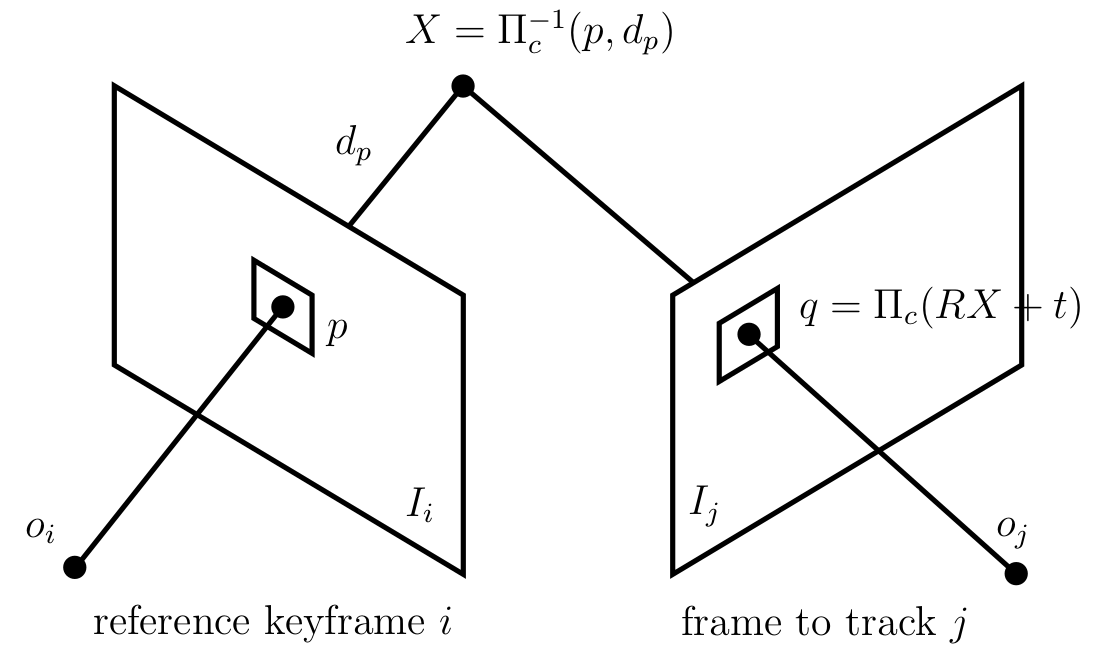
\includegraphics[width=\linewidth]{assets/img/direct-image-alignment.png}
	\caption{Direct image alignment}%
	\label{fig:direct-image-alignment}
\end{figure}

\begin{figure}[ht]
	\centering
	\includegraphics[width=\linewidth]{assets/img/energy-warp.png}
	\caption{Energy formulation for direct image alignment}%
	\label{fig:energy-warp}
\end{figure}

\begin{figure}[ht]
	\centering
	\includegraphics[width=\linewidth]{assets/img/energy-gauss-newton.png}
	\caption{Energy formulation for Gauss-Newton minimization}%
	\label{fig:energy-gauss-newton}
\end{figure}

\begin{figure}[ht]
	\centering
	\includegraphics[width=\linewidth]{assets/img/gauss-newton-step.png}
	\caption{Gauss-Newton step}%
	\label{fig:gauss-newton-step}
\end{figure}

\subsection{RGB-D Visual Odometry}%
\label{sub:rgbd-visual-odometry}

\begin{figure}[ht]
	\centering
	\includegraphics[width=\linewidth]{assets/img/kinect.jpg}
	\caption{Kinect sensor}%
	\label{fig:kinect}
\end{figure}

\section{Visual SLAM}%
\label{sec:v-slam}

\begin{figure}[ht]
	\centering
	\includegraphics[width=\linewidth]{assets/img/lsd-slam.png}
	\caption{LSD-SLAM}%
	\label{fig:lsd-slam}
\end{figure}

\subsection{Pose Graph}%
\label{sub:pose-graph}

\begin{figure}[ht]
	\centering
	\includegraphics[width=\linewidth]{assets/img/pose-graph.png}
	\caption{Pose graph}%
	\label{fig:pose-graph}
\end{figure}

\subsection{Loop Closure}%
\label{sub:loop-closure}

\begin{figure}[ht]
	\centering
	\includegraphics[width=\linewidth]{assets/img/loop-closure-lowres.png}
	\caption{Loop closure}%
	\label{fig:loop-closure}
\end{figure}

\chapter{Contribution on Visual Odometry}%
\label{cha:vors}

Explain vors (pas encore publié).

\begin{itemize}
	\item RGB-D Tracking Evaluation
	\item Visual Odometry in Rust (vors)
	\begin{itemize}
		\item Candidate points selection (coarse to fine)
		\item Multi-resolution image gradients
		\item Multi-resolution direct image alignment
		\item Levenberg-Marquardt (non-linear optimization)
		\item Gradients of the reprojection function (inverse compositional)
		\item Robust optimization techniques
		\item Photometric term in the residuals
	\end{itemize}
\end{itemize}

\chapter{Performant Web Applications}%
\label{cha:performant_web_applications}

\minitoc%

\section{A Brief History of Native Code in the Client}%
\label{sec:native_client}

\begin{figure}[h]
	\centering
	\includegraphics[width=\linewidth]{assets/img/wasm-timeline.pdf}
	\caption{Events releated to the birth and growth of WebAssembly.}%
	\label{fig:wasm-timeline}
\end{figure}

Being able to run high performance code in the browser
unlocks many use cases, including scientific computing.
Yet, it remains a challenging task.
Resources often refers to this as ``native'' code
but the terminology is rather vague.
Depending on the context, it may have one of the following meanings,
\begin{enumerate}
\setlength\itemsep{-0.5em}
	\item code statically compiled directly to the target architecture and running from the browser,
	\item code compiled from a typical ``native'' language such as C or C++,
	\item or anything that is not generating JavaScript.
\end{enumerate}
The distinction between those and how they relate to ``native'' code
will be made clearer after a brief history of high performance code in browsers.

\subsection{Java Applets}%
\label{sub:java_applets}

In 1995, just four years after the birth of the Web,
the Java programming language was created.
It appeared with a companion technology called Java Applet,
designed to run Java applications in the browser.
The Java Virtual Machine (JVM) was hosted by browsers,
enabling much better performances than JavaScript at this time.
As an example, Brendon C. Glazer worked on interactive ray tracing
of VRML scenes with Java applets in 1999~\cite{Glazer1999InteractiveRT}.
Figure~\ref{fig:glazer-thesis} depicts how the applet would appear
in a Web page at that time.
Since 1998 Java applets have also had access to 3D hardware acceleration~\cite{Java3dAPISpec}
whereas JavaScript waited until 2011 for WebGL in HTML5 canvas.

\begin{figure}[h!]
	\centering
	\includegraphics[width=\linewidth]{assets/img/glazer-thesis.jpg}
	\caption{Interactive ray tracing applet from Brendon C. Glazer master thesis (1999).}%
	\label{fig:glazer-thesis}
\end{figure}

On the down side, Java applets would break accessibility of the Web.
Screen readers would not be able to parse the content of the dedicated
applet area in the page.
The security model of Java applets was also quite risky.
Applets would have to get approved by a browser user and then gain rights
equivalent to a native application on your desktop.
Unfortunately, just like terms of service, most people just click ``agree''
and move on.
In addition, the Java Runtime Environment (JRE) has had hundreds security
vulnerabilities~\cite{JreCve} in its lifetime.
This represents a serious security threat for browser vendors.
Java applets were eventually entirely removed from Java SE 11, in 2018.

\subsection{Flash}%
\label{sub:Flash}

In his ``History of Flash''~\cite{HistoryFlash}, Jonathan Gay retraces the early days of Flash.
In 1993, he, Charlie Jackson and Michelle Welsh founded FutureWave Software
but their initial vector drawing application did not draw much attention (pun intended).
After discussions at Siggraph 1995, the company decided to focus on a web animation
product named ``FutureSplash Animator''.
It gained reputation with Microsoft and Disney using it and as a consequence,
was acquired by Macromedia and rebranded ``Flash'' in 1996.

Contrary to Java applets, Flash use cases started very narrow.
It provided a simple and efficient solution to build and share animations on the web,
giving a visual advantage over pure HTML documents.
In year 2000, Flash 5 was released, with the ActionScript programming language,
bringing even more potential to Flash-based websites.
Two years later, in 2002, Flash 6 brought support for real-time messaging protocols,
enabling video and audio streaming capabilities.
This represents roughly 8 years until 2010 when such capabilities are also
supported through HTML5 in most browsers.
In the meantime, highly influencial projects shaped the Web thanks to Flash.
You may have heard of Chad Hurley, Steve Chen and Jawed Karim who launched
YouTube in 2005, based on Flash.

In spite of the many advantages of Flash and ActionScript over classic Web pages,
it also had similar flaws than Java applets.
In October 2000, usability consultant Jakob Nielsen published a short article
entitled ``Flash: 99\% Bad''~\cite{FlashBadNielsen} stating that
``Flash technology tends to discourage usability for three reasons:
it makes bad design more likely,
it breaks with the Web's fundamental interaction style,
and it consumes resources that would be better spent enhancing a site's core value.''
Apple also played a huge role in Flash decline.
In 2007 the iPhone launched without Flash support,
leading to Steve Jobs, then Apple CEO, writing in 2010 an oppen letter called
``Thoughts on Flash''~\cite{FlashJobs}
in which he explains why Flash was doomed to disappear.
Among those reasons, Flash is proprietary, going against open Web standards,
it has numerous security flaws~\cite{FlashCVE}, and is the number one reason Macs crash.

Consequently, with the advent of HTML5 surrounding technologies regarding multimedia capabilities,
and the improved performances of JavaScript, Flash became obsolete.
So in July 2017, Adobe announced end support for Flash in 2020.

\subsection{Google Native Client (NaCl)}%
\label{sub:nacl}


------------------------- NaCl

Native Client (NaCl) project in chrome
A lot of C and C++ code already written.
Secure execution of native code.
-> Changing the compiler to produce only "secure" code, inside a sandbox.
-> no plugin "please install"
-> check at runtime if the application respect the safety rules, or shutdown.

Plugins have historically been the number one source of web browser vulnerabilities.

Pepper API, mirror of the Browser API, for NaCl code.
built-in flash using Pepper and Pdf reader using Pepper.

NaCl is architecture specific. Started with the GCC toolchain.
Need to go through the Chrome web store.

PNaCl 2013.
https://blog.chromium.org/2013/10/chrome-31-beta-android-application.html
PNaCl, an intermediate representation, compile on the fly. Uses Clang.
Based on the LLVM toolchain.

Focused on desktop, no mobile for now.

------------------------

Java and Flash are technologies owned by companies, this does not integrate well with the Web.
Asm.js was just JS. "Don't break the web".
WebAssembly is a W3C spec, it went through the process, not against it.
Wasm is also small. Flash and Java Applets needed to download a runtime. and PNaCl was built
on top of LLVM IR, a bit unstable.
Wasm does not force you to use a specific language like Flash or Java.

Wasm has security in mind, it runs in the same sandbox than JS.

\section{Emscripten}%
\label{sec:Emscripten}

Faisons un bref détour "historique". Alon Zakai, qui travaille à Mozilla, a démarré un projet perso autour de 2010 par curiosité (vidéo, autre vidéo). Il se demandait s’il était possible de transformer du code C++ en du code JavaScript pour le faire tourner dans un navigateur. C’est le début de emscripten. Emscripten transforme du code LLVM en JavaScript. LLVM est ce qu’on appelle une représentation intermédiaire (IR) qui permet à du code humain (C++, rust, ...) d’être transformé en code LLVM qui lui même est après transformé en code spécifique à une architecture (32 bits, 64 bits x86 intel, ARM, embarqué, ...).

Et donc ce que Alon Zakai a démarré en 2010 c’est une nouvelle "cible" : JavaScript. Initialement c’était assez lent, loin d’être optimisé. Après quelques itérations, avec l’aide de Luke Wagner qui travaillait sur le compilateur JavaScript, ils ont formalisé une syntaxe spécifique. Un sous-ensemble de JavaScript qui peut être facilement reconnu par le compilateur du navigateur et optimisé bien plus efficacement. Cette syntaxe ressemblait à ça

function sum(x, y) {
    var x = x | 0;  // x is a 32-bit value
    var y = y | 0;  // so is y
    return (x+y) | 0; // 32-bit addition, no type or overflow checks
}

Normalement, lorsque l’on fait x + y en JavaScript, le compilateur doit vérifier les types des deux variables dynamiquement choisir la bonne opérations somme en conséquence. Le faire au runtime est très coûteux. Alors qu’avec cette syntaxe, formalisée sous le nom de asm.js, le compilateur peut directement émettre l’instruction processeur de somme de deux entiers 32 bits. Après avoir intégré la techno avec des équipes de Unity et Unreal pour faire tourner leur moteur de jeu dans le navigateur, la preuve de concept était faite. Il s’en est suivi un peu de diplomatie entre les gros du web (Google, Microsoft, Mozilla) pour formaliser WebAssembly, le successeur de asm.js.

Ce petit détour permet de comprendre ce qu’est emscripten, comment le projet à évolué jusqu’à aujourd’hui où on peut l’utiliser pour compiler du code C/C++ vers wasm. La clé de la compréhension c’est ce schéma :

Code source (C++) -> LLVM IR -> Emscripten -> WebAssembly

Donc Emscripten a besoin du bitcode LLVM pour pouvoir compiler une base de code C++. En particulier, il n’est pas possible d’utiliser les bibliothèques précompilées (les “.so”) fournies par les OS dans les packages (apt-get install ...) dans ses dépendances. Toute dépendance (et ce récursivement) doit être recompilée avec Emscripten depuis le code source, et liée statiquement à la compilation de notre propre code. Par défaut, pour faciliter la vie, Emscripten intègre déjà la majorité de la librairie standard (std), et de certaines autres bibliothèques (SDL pour les applis graphiques, ...).


\begin{itemize}
	\item LLVM
	\item asmJS
	\item wasm
\end{itemize}

\section{WebAssembly}%
\label{sec:WebAssembly}

\begin{itemize}
	\item Minimum Viable Product (MVP)
	\item Bright future: wasi, wapm, ...
\end{itemize}

\section{C++ portability pitfalls}%
\label{sec:cpp_pitfalls}

Example with image reading in OpenCV.
Had to rewrite PNG decoder.


DVO par exemple a des dépendances à OpenCV, Eigen, Boost, et Sophus. J’ai donc commencé par voir si j’arrive à compiler un programme minimaliste OpenCV avec Emscripten. Tout de suite les ennuis ont démarré. Au début, je n’ai même pas réussi à utiliser le build wasm de OpenCV (cf question sur stackoverflow). Je m’en suis finalement sorti, pour bloquer sur l’étape d’après, lire une image (cf question sur le forum OpenCV). En effet, dans la version wasm de OpenCV, la fonction imread a été remplacée par une méthode purement JavaScript qui prend un canvas en paramètre, et va donc directement récupérer la matrice depuis le canvas sans faire le décodage. Je pense que cette stratégie a été utilisée parce qu’en interne, la fonction imread OpenCV utilise la fonction imdecode, qui elle-même fait appel à une douzaine d’autres bibliothèques (libjpeg, libtiff, libpng, ...). J’ai essayé d’ajouter moi-même le module contenant la fonction imdecode au build wasm d’OpenCV mais je n’ai pas réussi à compiler ce module. J’ai tout un tas d’erreurs de "missing symbol" etc.

Ce n’est pas entièrement sans espoir, il faut le savoir ! Notamment, je n’ai besoin que du décodage png. Et libpng fait partie de ces quelques lib déjà intégrées à emscripten. En théorie je pourrais donc remplacer le code de décodage (cv::imdecode) par l’utilisation de libpng directement. Un des soucis c’est que l’API de libpng est super difficile à comprendre pour moi. Mais en théorie, le reste d’OpenCV qui est utilisé dans DVO fait partie du sous-ensemble qui devrait marcher.

Par contre, je n’ai pas fait de tests minimalistes avec les autres dépendances de DVO (eigen, boost, sophus) donc rien ne dit qu’on serait au bout de nos ennuis.

\section{Rust and WebAssembly}%
\label{sec:rust_wasm}

\begin{itemize}
	\item Rust programming language
	\item Wasm-bindgen
\end{itemize}

\chapter{Interactive Visual Odometry on the Web}%
\label{cha:interactive_vo_on_the_web}

\minitoc%
\clearpage

\section{Visual Odometry in Rust (VORS)}%
\label{sec:vors}

\subsection{Overview of VORS}%
\label{sub:vors-overview}

VORS is a sparse, keyframe-based, RGB-D, direct visual odometry algorithm.
As presented in Section~\ref{sub:appearance-based},
VORS belongs to the family of direct visual odometry,
based on the image alignment optimization problem.
Contrary to monocular visual odometry, which requires an estimation
of points depth, we focus on the RGB-D case,
where the necessary depth information for reprojection is provided by a sensor.
In order to reduce drift when the camera moves slowly,
image alignment is performed from a fixed keyframe instead of the previous frame.
Decision to change the keyframe is done heuristically;
details are presented in Section~\ref{sub:multi-res-direct-image-alignment}.
Finally, our algorithm uses a sparse subset of points in the image,
which has been shown~\cite{engel2017direct} to be sufficient to track the camera motion.
Disregarding sparsity and robustness, discussed later,
our algorithm is very similar to DVO~\cite{kerl2013robust},
and its predecessor~\cite{steinbrucker2011real}.
An overview of the full pipeline of VORS is presented in Figure~\ref{fig:overview-vors}.

\begin{figure}[ht]
	\centering
	\includegraphics[width=\linewidth]{assets/img/overview-vors.pdf}
	\caption{Overview of VORS pipeline.}%
	\label{fig:overview-vors}
\end{figure}

\subsection{Sparse Points Selection}%
\label{sub:sparse-points}

Engel et al.\ demonstrated in DSO~\cite{engel2017direct} that using a sparse subset
of points for the direct image alignment problem still results in precise camera locations
at the condition that points satisfy two conditions,
\begin{itemize}
\setlength\itemsep{-0.5em}
	\item they should be well distributed in the image,
	\item and they should be located at positions with higher gradients magnitudes.
\end{itemize}
Selected points are called candidate points,
and their selection mechanism is rather complex, based on at least ten parameters.
The core idea is to regularly divide an image in tiles.
One subdivision produces big tiles, called regions,
and another generates small tiles, called blocks.
One pixel is selected per block if its gradient is higher than a local threshold
depending on the region containing the pixel.
In practice, blocks are actually multi-scale, with three default levels.
If none of the four ``level $n$'' blocks composing a ``level $(n+1)$'' block elected a candidate point,
the ``level $(n+1)$'' block checks whether a pixel satisfies a lower threshold.
The factor between block thresholds at different levels is one of the parameters.
Another mechanism aims at obtaining a target amount of candidate points.
That amount can be approximated from blocks base size but it might differ.
Depending on the difference with the target count,
the algorithm will choose between the three following options,
(1) keep candidates, (2) randomly select a sample of the candidates,
or (3) change the block base size and restart from scratch.

In contrast, our sparse selection of candidates is rather simple,
based on a multi-resolution pyramid of images.
We embraced the idea that each level of the image pyramid should exhibit
that property of well distributed points with higher density near higher gradients.
% Intuitively, it should help convergence of the alignment problem to a global minimum.
We thus propose a simple coarse-to-fine selection mechanism,
depicted in Figure~\ref{fig:coarse-to-fine-candidates}.
At the lowest resolution, all points are candidates.
For each candidate pixel at one pyramid level, we elect one or two candidates
in the four subpixels of the next level.
A threshold based on gradients is used to determine which pixels should be selected.
This sparse selection scheme ensures that there is at least one candidate per region
corresponding to one pixel at the lowest resolution.
It also increases the density of candidates in higher gradients areas.
The number of levels of the image pyramid is a common parameter for candidates selection
and for the multi-resolution direct image alignement presented next.

\begin{figure}[ht]
	\centering
	\includegraphics[width=0.23\linewidth]{assets/img/candidates-icl-4.png}
	\hfill
	\includegraphics[width=0.23\linewidth]{assets/img/candidates-icl-3.png}
	\hfill
	\includegraphics[width=0.23\linewidth]{assets/img/candidates-icl-2.png}
	\hfill
	\includegraphics[width=0.23\linewidth]{assets/img/candidates-icl-1.png}
	\caption{Coarse-to-fine candidate selection of VORS.
	Candidates are represented in red.
	All points are kept at the lowest resolution.
	Each higher resolution elects one or two candidates per parent candidate.}%
	\label{fig:coarse-to-fine-candidates}
\end{figure}

Figure~\ref{fig:candidates-dso-vors} depicts a zoomed-in view of the same image region
for both DSO and VORS candidates selection mechanisms.
As visible on the left image, DSO candidate points are regularly spaced,
except in homogenous areas.
VORS candidate points however tend to form contiguous lines,
which probably generates redundant information.
Limiting the maximum number of subpixel candidates to one
at some levels (in the higher resolutions),
could both help control the maximum amount of candidates and
limit the information redundancy generated by neighbour candidates.

\begin{figure}[t]
	\centering
	\includegraphics[width=0.49\linewidth]{assets/img/candidates-icl-dso-cropped.png}
	\hfill
	\includegraphics[width=0.49\linewidth]{assets/img/candidates-icl-vors-cropped.png}
	\caption{DSO (left) and VORS (right) candidate points (in red).}%
	\label{fig:candidates-dso-vors}
\end{figure}

\subsection{Multi-Resolution Direct Image Alignment}%
\label{sub:multi-res-direct-image-alignment}

\subsubsection{Convergence of the Optimization Problem}%
\label{ssub:convergence-optimization}

As presented in Section~\ref{sub:appearance-based},
under the photoconsistency assumption, direct image alignment consists
in finding the warp function $W$ minimizing
\[
	\sum_{\bm{x}}\|I(W(\bm{x})) - I^{*}(\bm{x})\|^2
\]
where $I^{*}, I$ are the reference and new images,
and $\bm{x}$ is the position of a pixel in the reference image.
As explained in Baker and Matthews~\cite{baker2004lucas},
this can be minimized with an iterative optimization.
If we note $\bm{\xi}$ the parameters of the warp function,
and $\delta\bm{\xi}$ the iterative increments,
the expression of the residual in an inverse compositional formulation is
\[
	I^{*}(W(\bm{x}, \delta \bm{\xi})) - I(W(\bm{x}, \bm{\xi})).
\]
In a Gauss-Newton scheme, the iterative increment $\delta\bm{\xi}$ is computed as
\[
	\delta \bm{\xi} = \inv{H} \sum_{\bm{x}} \tr{J} (I^{*}(\bm{x}) - I(W(\bm{x}, \bm{\xi})))
\]
where $J = \nabla I \cdot J_{\bm{\xi}}W$, $\nabla I$ is the image gradient
and $J_{\bm{\xi}}W$ is the Jacobian of the warp function.
The Hessian is computed as the Gauss-Newton approximation
$H = \sum_{\bm{x}}\tr{J}J$.
We parameterize $W$ in the Lie algebra of twists $\seee$.
The expression of the Jacobian of the warp function
is detailed in Appendix~\ref{sec:notation}.

In theory however, this iterative algorithm is only correct under the assumption
that the initialization is already near the solution.
Convergence to the correct minimum is thus a hard problem
and under some circumstances, the optimization may drift to another local minimum.
One way to help convergence is to use the Levenberg-Marquardt approximation
of the Hessian.
It consists in multiplying the diagonal elements of
the Gauss-Newton approximation of the Hessian by $(1 + \lambda_{lm})$.
The Levenberg-Marquardt coefficient $\lambda_{lm}$ is dynamically
updated toward 0 when converging or toward $+\infty$ when diverging.

Another method to improve convergence consists in solving the optimization
with a coarse-to-fine multi-resolution approach.
Indeed, the image gradient used for the Jacobian contains information
of larger areas of the original image when computed at lower resolutions.
As a consequence, the vicinity of the global optimum is artificially increased.
For the direct image alignment, we thus use a pyramid of images,
where each level has half the resolution of the previous one.
As explained previously the number of levels also impacts candidate points selection.
Indeed, at the lowest resolution, all pixels serve as candidates for the optimization.
The number of levels is thus chosen as a compromise between the minimum amount
of candidate points and the desired convergence rate.
Starting from 640x480 images in the ICL-NUIM and TUM RGB-D datasets,
we found that 6 levels is a good compromise.
The lowest resolution has 20x15 images, which implies a minimum of 300 candidate points.

\subsubsection{Multi-Resolution Intrinsics}%
\label{ssub:multires-intrinsics}

Since we use a coarse-to-fine optimization,
we must be able to initialize one level from the result of the previous one.
In Section~\ref{sub:intrinsic_parameters}, we presented the image formation as
the succession of two transformations, first the projection from the camera frame
to the image frame, and then the projection onto the pixels frame.
When halving the image resolution, the second transformation $K_s$ changes.
\[
	K_s = \begin{pmatrix}
		s_x & s_{\theta} & o_x \\
		0 & s_y & o_y \\
		0 & 0 & 1 \\
	\end{pmatrix}.
\]
We note $K_s'$ the new pixels projection with a resolution multiplied by $\alpha$.
In our case $\alpha$ is of the form $2^{-n}$.
On the one hand, scaling parameters are all multiplied by $\alpha$ i.e.\
$s_x' = \alpha s_x$,
$s_y' = \alpha s_y$ and
$s_{\theta}' = \alpha s_{\theta}$.
The principal point parameters on the other hand depend on the origin of the coordinate system.
In most modelizations, the value of pixel $(x,y)$ is interpreted as the integration
of the light hitting the sensor on the surface located between $(x-0.5, y-0.5)$
and $(x+0.5, y+0.5)$.
The coordinates of the top left corner of the image is thus $(-0.5, -0.5)$
instead of $(0,0)$.
Figure~\ref{fig:multiscale-intrinsics} illustrates how
the principal point is transformed in such coordinate system.
As a result, the location of the principal point is updated as
$o_x' = \alpha(o_x + 0.5) - 0.5$ and
$o_y' = \alpha(o_y + 0.5) - 0.5$.
In the end, the updated intrinsic pixel transformation is
\[
	K_s' = K_{\alpha}K_s \quad \text{with} \quad
	K_{\alpha} = \begin{pmatrix}
		\alpha & 0 & 0.5(\alpha - 1) \\
		0 & \alpha & 0.5(\alpha - 1) \\
		0 & 0 & 1 \\
	\end{pmatrix}.
\]

\begin{figure}[t]
	\centering
	\includegraphics[width=\linewidth]{assets/img/multiscale-intrinsics.pdf}
	\caption{Effect of a centered coordinate system on
	the coordinates of the principal point at multiple resolutions.}%
	\label{fig:multiscale-intrinsics}
\end{figure}

The presented approach is the one used by the TUM RGB-D coordinate system
for the principal point given in the intrinsics matrix.
It is thus also the one we use when initializing the multi-resolution intrinsic
parameters in step 2 of Figure~\ref{fig:overview-vors}.
The camera motion estimated at one resolution can thus be reused as-is
for the initialization of the next resolution.
It is the projection that changes, due to a different intrinsic matrix.

\subsubsection{Keyframe Update}%
\label{ssub:keyframe-update}

We mentioned in VORS overview that the decision to change the keyframe is done heuristically.
Similarly to ORB-SLAM~\cite{mur2015orb} and DSO~\cite{engel2017direct},
we use the optical flow of tracked points, which is
the distance in pixels between their locations in the reference and in the tracked images,
to make that decision.
For convergence reasons, we established that the reference and the tracked frames
should not be too different from each other.
We therefore use a mean threshold distance of one pixel at the lowest image resolution.


\subsection{Limits of the Implementation}%
\label{sub:limits-implementation}

To our knowledge,
VORS is the first Rust-only complete direct visual odometry stack.
We thus value simplicity for this important milestone.
Incidentally, our algorithm lacks a few significant features,
left as later improvements.

One notable missing component is robustness to outliers.
It is common that the photoconsistency assumption does not hold with real-world images.
Among the many possible reasons, two of them are the presence of dynamic moving objects,
and the appearance of bright spots due to light reflections.
One possible solution is to use a robust M-estimator instead of a least square estimation.
The energy to minimize then takes the form
\[
	\sum_{\bm{x}}\rho(I(W(\bm{x})) - I^{*}(\bm{x}))
\]
where $\rho$ has a few interesting properties.
In part 2 of their series on direct image alignment~\cite{baker2003lucas},
Baker et al. explain in details how a robust M-estimator can be used
within an inverse compositional iteratively reweighted least squares (IRLS) algorithm.
Possible estimators include Huber, Geman-McClure, Tukey or even t-distribution estimators.
Klose et al.~\cite{klose2013efficient} use Huber and Tukey M-estimators,
while for example, Kerl et al~\cite{kerl2013robust}
and Gutierrez et al.~\cite{gutierrez2015inverse} prefer the t-distribution.

Another commonly appearing problem with cameras is automatic exposure variations.
With changes in lighting conditions,
exposure parameters of cameras are often automatically adjusted,
resulting in global photoconsistency errors.
Different affine exposure parameterizations have successfully been integrated
in the expression to minimize, such as in~\cite{klose2013efficient} and~\cite{engel2017direct}.
We did not add such additional parameters in our modelization
and thus expect VORS to have difficulties tracking the camera motion
in scenes with brightness changes.


\section{RGB-D Visual Odometry Evaluation}%
\label{sec:rgbd-vo-evaluation}

As previously explained, our implementation
belongs to the family of direct visual odometry from RGB-D images.
In this section, we will detail how it has been evaluated against
comparable algorithms by introducing the available datasets,
presenting the different evaluation metrics,
and finally lay out the testing setup we provide with the evaluation results.

\subsection{Dataset Creation / Acquisition}%
\label{sub:dataset_creation}

Comparing different algorithms is a complex task for many reasons,
one of them being the ability to run those algorithms on the same set of data.
The existence of well built reference datasets is thus a crucial point,
and understanding their characteristics is valuable to correctly compare and interpret
evaluation results.

\subsubsection{Overview of Available Datasets}%
\label{ssub:datasets_overview}

We saw in Chapter~\ref{cha:the_image_annotation_problem} that the principal
difficulty for building annotation datasets is the required human annotation time.
For visual odometry, algorithms are strongly related to capture devices,
be it stereo, mono, RGB-D cameras, or cameras paired with other sensors
such as inertial measurement units (IMU), GPS or lidar.
As a consequence, different datasets focus on different acquisition systems.
For every evaluated acquisition system, there must exist another measurement system,
more precise and reliable than the one being evaluated.
The main difference is thus that
the challenge is technological for visual odometry,
while it is mostly time consumption for image annotation.

The availability of datasets for visual odometry first came from the mobile robotics community,
mostly interested in SLAM from laser sensors (lidar).
The data is thus collected from sensors attached to a mobile robot or a car.
In the New College~\cite{smith2009new} and NCLT~\cite{carlevaris2016university} datasets,
the robotic platform is based on a Segway, the KITTI dataset~\cite{geiger2013vision}
recorded data from a sensors equipped car,
while the EuRoC MAV~\cite{burri2016euroc}
dataset is based on a micro aerial vehicle (MAV).
These platforms are depicted in Figure~\ref{fig:mobile-robot-slam}.
The ground truth was recorded with three different approaches for these datasets.
Visual odometry ground truth was an after thought for the New College dataset,
only available a year later on their website and not discussed in the paper.
It appears to have been obtained from dead-reckoning, i.e.\ from wheel and IMU odometry,
provided by the Segway platform, and is thus not very reliable.
In the NCLT dataset, the mobile robot trajectory ground truth is computed from
a high precision realtime kinematic GPS (RTK GPS) and a graph SLAM based on lidar measurements.
The accuracy of the trajectory ranges from a centimeter to a decimeter approximately for a total
travelled distance of roughly 147 km.
The ground truth trajectory of the KITTI dataset was also obtained from high precision
GPS/IMU sensors and is thus also accurate at the decimeter scale.
The setup for the EuRoC MAV dataset is a bit different since the mobile vehicle
is flying in indoor environment and its trajectory is obtained from motion capture devices.
The total travelled distance is thus way shorter, less than a kilometer,
but the trajectories are accurate at approximately a millimeter.

\begin{figure}[ht]
	\centering
	\includegraphics[height=0.3\linewidth]{assets/img/new-college.png}
	\hfill
	\includegraphics[height=0.3\linewidth]{assets/img/nclt.png}
	\hfill
	\includegraphics[height=0.3\linewidth]{assets/img/euroc-mav.png}
	\caption{Mobile robots used for SLAM datasets. From left to right,
	the Segway platform used in the New College dataset~\cite{smith2009new},
	the Segway platform used in the NCLT dataset~\cite{carlevaris2016university},
	the MAV used in the EuRoC MAV dataset~\cite{burri2016euroc}.}%
	\label{fig:mobile-robot-slam}
\end{figure}

A second wave of datasets,
represented in bold in Table~\ref{tab:vo-datasets},
has especially been targetting RGB-D cameras,
becoming popular after the launch of the Microsoft Kinect.
While the TUM RGB-D~\cite{sturm2012benchmark} and Bonn RGB-D~\cite{palazzolo2019iros}
datasets are recorded with real RGB-D sensors,
the ICL-NUIM~\cite{handa2014benchmark} dataset was generated (ray-traced rendered)
from synthetic 3D models of indoor scenes.
We are going to explain in more details the specificities of the TUM RGB-D and
ICL-NUIM datasets since these are the two we used to evaluate our direct RGB-D
visual odometry algorithm.

Finally, with the popularity of inertial sensors coupled with cameras in
modern smartphones enabling new augmented reality functionalities,
a regain in interest has been visible for 6 degrees of freedom visual inertial odometry (VIO).
While the EuRoC MAV~\cite{burri2016euroc} and TUM VI~\cite{schubert2018tum} datasets
are using high quality sensors,
the ADVIO dataset~\cite{cortes2018advio} is actually using regular smartphones sensors,
showing the importance of datasets with less precise data to improve algorithms robustness.
We provide a brief summary of these datasets properties in Table~\ref{tab:vo-datasets}.
Note that this is not an exhaustive list of available datasets but an overview
of the main ones for visual odometry.

\begin{table}[ht]
\centering
\resizebox{\textwidth}{!}{%
\begin{tabular}{llll}
Dataset
	& Year
    & Available data
	& Ground truth \\
    \midrule
New College~\cite{smith2009new}
	& 2009
	& \makecell[l]{GPS, IMU, wheel odometry,\\lidar, omnidirectional, stereo}
	& Dead-reckoned \\
\textbf{TUM RGB-D~\cite{sturm2012benchmark}}
	& 2012
	& IMU, \textbf{RGB-D}
	& Motion capture \\
KITTI~\cite{geiger2013vision}
	& 2013
	& GPS, IMU, lidar, stereo
	& High precision GPS/IMU \\
\textbf{ICL-NUIM~\cite{handa2014benchmark}}
	& 2014
	& \textbf{RGB-D}, 3D surface
	& Synthetic \\
NCLT~\cite{carlevaris2016university}
	& 2016
	& \makecell[l]{GPS, IMU, wheel odometry,\\lidar, omnidirectional}
	& RTK GPS and lidar SLAM \\
EuRoC MAV~\cite{burri2016euroc}
	& 2016
	& Stereo camera
	& Motion capture \\
TUM Mono~\cite{engel2016photometrically}
	& 2016
	& Mono camera
	& Closed loop \\
TUM VI~\cite{schubert2018tum}
	& 2018
	& IMU, Mono camera
	& Motion capture and closed loop \\
ADVIO~\cite{cortes2018advio}
	& 2018
	& Smartphone IMU and video
	& IMU with position fixes \\
\textbf{Bonn RGB-D~\cite{palazzolo2019iros}}
	& 2019
	& IMU, \textbf{RGB-D}, lidar
	& Motion capture \\
\end{tabular}%
} % end of resizebox
\caption{Visual odometry datasets}%
\label{tab:vo-datasets}
\end{table}


\subsubsection{Motion Capture for RGB-D Visual Odometry}%
\label{ssub:motion_capture}

The TUM RGB-D dataset~\cite{sturm2012benchmark} was the first
complete and rigorously detailed dataset for RGB-D visual odometry.
It is composed of 80 sequences, 47 for training with ground truth,
and 33 for validation only evaluated online, without ground truth.
The training sequences are arranged in six groups,
\begin{itemize}
\setlength\itemsep{-0.5em}
	\item testing and debugging (4 sequences), simple translation or rotation movements,
	\item handheld movements (11 sequences),
	\item robot movements (4 sequences),
	\item structure and texture (8 sequences), with difficult structure or texture patterns,
	\item dynamic objects (9 sequences),
	\item and object reconstruction (11 sequences).
\end{itemize}
As we can see, the dataset provides both easy sequences and sequences with
more difficult situations such as dynamic movements or poor textures
in the field of view of the camera.
It is thus a good benchmark of the robustness of visual odometry algorithms.
These sequences have been acquired by three different Kinect devices,
named fr1 (for ``Freiburg 1''), fr2 and fr3.
All their intrinsic parameters are available in the dataset.
The required robustness of the tested algorithms is also increased by the fact that
the color camera of the Kinect sensor has a rolling shutter.
We do not expect our algorithm to perform very well under those circumstances.

The ground truth camera poses are obtained thanks to an external motion capture system
based on MotionAnalysis~\cite{MotionAnalysis} hardware and software.
This setup is composed of eight 300 Hz Raptor-E high definition cameras,
equipped with infrared lights to illuminate passive markers attached to the Kinect.
After a detailed intrinsic and extrinsic parameters calibration of the system,
the authors estimate the relative position errors to be lower than 1 mm and 0.5 degrees.

\subsubsection{Synthetic Dataset Creation}%
\label{ssub:synthetic_dataset}

Most of the available visual odometry datasets lack a dense 3D surface ground truth
to be able to evaluate both the camera trajectory and the structure reconstruction.
To this end, Handa et al.\ created the ICL-NUIM dataset~\cite{handa2014benchmark}.
Contrary to most other datasets, the video sequences provided here are completely
generated by computer graphics, using the open-source ray tracing algorithm
POV-Ray~\cite{povray}.
The dataset is split into two rooms, a living room and an office,
and two scenarios, one noiseless and one with simulated noise.
The full pipeline is also provided as open source,
if one wishes to customize parts of it.
The geometry and some renders of the living room are displayed in Figure~\ref{fig:icl-nuim}.

\begin{figure}[t]
	\centering
	\includegraphics[height=0.3\linewidth]{assets/img/icl-nuim-geometry.png}
	\hfill
	\includegraphics[height=0.3\linewidth]{assets/img/icl-nuim-povray.png}
	\caption{Geometry (left) and few rendered images (right)
	of the living room used for the ICL-NUIM dataset~\cite{handa2014benchmark}.}%
	\label{fig:icl-nuim}
\end{figure}

In order to test some visual odometry algorithms,
we are only going to use the eight noise-free sequences since realistic noisy sequences
are already evaluated with the TUM RGB-D dataset.
The trajectory ground truth generated by this ICL-NUIM dataset is thus error-free.
The color and depth images are also perfectly aligned,
timely synchronized and have no light exposure variations.
They still contain reflective surfaces and few other ligthing effects
not taken into account in our direct visual odometry modelization,
but the overall circumstances should be very favorable for our simple implementation.

\subsection{Evaluation Metrics}%
\label{sub:metrics}

There are basically two types of evaluation metrics,
those based on a ground truth, and those that are not.

\subsubsection{Metrics with Ground Truth, ATE and RPE}%
\label{ssub:metrics_gt}

The most straightforward method to evaluate a visual odometry trajectory
is to compare it with a reference trajectory, called ground truth.
This reference trajectory needs to be acquired with more precision
than the one being evaluated for the measure to make sense.
In our case, the TUM RGB-D dataset uses a motion capture system with sub-millimeter accuracy,
and the ICL-NUIM provides exact trajectories since it is a synthetic dataset.

The first evaluation metric commonly used is the absolute trajectory error (ATE).
We can consider the trajectory as a discrete set of camera poses
\[
	G_{\Omega} = \Set{g_{\tau}}{\tau \in \Omega,\ g_{\tau} \in SE(3)}
\]
where $\Omega$ is the set of discrete time events when camera poses are available.
In theory, the ATE can be computed as
\[
	\text{ATE} = \sum_{\Omega} d(g_{\tau}, \widehat{g}_{\tau})
\]
where $d(g_{\tau}, \widehat{g}_{\tau})$ can be thought of
as a distance between the estimated transformation $g_{\tau}$
and the ground truth transformation $\widehat{g}_{\tau}$.
Usually, we can consider two types of errors, the translation error
\[
	\| \text{trans}(\inv{\widehat{g}_{\tau}} \cdot g_{\tau}) \|
\]
and the rotation error
\[
	\measuredangle \, (\inv{\widehat{g}_{\tau}} \cdot g_{\tau})
\]
where $\measuredangle$ is the amplitude ($\geq 0$) of the rotation angle.
Since the rotation errors will also impact translation errors later,
it is common to only use the translation error when computing the ATE.
The two most widely used ATE metrics are the RMSE and the median scores
\[
	\text{ATE}_{\text{rmse}} =
		\left(
			% \frac{1}{\text{Card}(\Omega)} \sum_{\Omega}
			\mean
			{\| \text{trans}(\inv{\widehat{g}_{\tau}} \cdot g_{\tau}) \|^2}
		\right)^{1/2}
	\quad \text{and} \quad
	\text{ATE}_{\text{median}} =
		\text{median} \left( \| \text{trans}(\inv{\widehat{g}_{\tau}} \cdot g_{\tau}) \| \right).
\]
The median is a better indicator of the algorithm precision,
while the RMSE better reflects the presence (or absence) of outliers,
i.e.\ the global robustness of the algorithm.

In practice, we should note that the ground truth and estimated trajectory
are not expressed in the same reference frame.
It is thus necessary to first align the two trajectories.
This is usally done with a principal component analysis (PCA)
of the trajectories.
It is also important to note that the ground truth and estimated trajectories
are not sampled at the same timings and frequency.
Therefore, it is also necessary to correctly associate poses of each trajectory,
which is reasonably easy when timestamps have been synchronized in the dataset.
One of the main issues of the ATE is that drifts have higher impact at the beginning
of the sequence than at the end.
To better evaluate long sequences we thus use another metric,
the relative pose error (RPE).

Contrary to the ATE, which evaluates absolute errors on associated pairs of poses,
the RPE compares the relative motion in a sliding window along the sequence.
The size of the window is usually a fixed travelled distance or time interval.
We will detail for example the computation of the RPE at 1 second.
For each associated pair of estimated and ground truth poses $(g_{\tau}, \widehat{g}_{\tau})$,
we consider another pair $(g_{\tau'}, \widehat{g}_{\tau'})$
delayed by 1 second ($\tau' \approx \tau + 1s$).
The camera motion between $\tau$ and $\tau'$ in the estimated trajectory is
$\Delta_{\tau \tau'} g = \inv{g_{\tau}} \cdot g_{\tau'}$
and the camera motion in the ground truth trajectory is
$\Delta_{\tau \tau'} \widehat{g} = \inv{\widehat{g}_{\tau}} \cdot \widehat{g}_{\tau'}$.
The relative pose error is thus computed as
\[
	\text{RPE} = \sum_{\Omega'} d(\Delta_{\tau \tau'} g, \Delta_{\tau \tau'} \widehat{g})
\]
where $d(\cdot, \cdot)$ is similar than for the ATE,
and $\Omega'$ is the set of regularly spaced pairs,
whether it is a duration, like 1 second, or a distance like 1 meter.

\alert{Ajouter un schéma RPE avec les notations précédentes.}


\subsubsection{Metrics without Ground Truth}%
\label{ssub:metrics_no_gt}

In some conditions, such as long handheld outdoor trajectories,
retrieving a ground truth might be problematic.
Yet it is still possible to partially evaluate the precision of an algorithm,
or rather its robustness to drifts and losses.
Indeed, in absence of a full sequence ground truth,
it is still possible to evaluate the tracking of loops.
It is important to note that global loop closure detections must
be deactivated in the algorithms for these measures to make sense.

One method consists in computing loop closure and pose graph optimization
and then compare the trajectory before and after.
If the drifts of the tracking are not too extreme and do not prevent the pose graph optimization,
this error can be representative of the visual odometry performance.

Another approach consists in specifically designing the dataset sequences
to start and end at the same location, such that both ends of the trajectory
can be precisely aligned.
This is the approach taken in~\cite{engel2016photometrically}.
The error computed is then the accumulated drift between the sequence when aligned
to the start and when aligned to the end of the partial ground truth trajectory.


\subsection{Setup and Algorithms Evaluation}%
\label{sub:algorithms_eval}

In this section, we describe how we evaluated our VORS implementation
and compared it to other open source C++ algorithms.
We focused on RGB-D visual odometry, and therefore used
both the TUM RGB-D~\cite{sturm2012benchmark} and ICL-NUIM~\cite{handa2014benchmark} datasets.

\subsubsection{The TUM RGB-D Dataset Format}%
\label{ssub:dataset-format}

The TUM RGB-D dataset is well specified and as a result,
others including ICL-NUIM follow the same format.
We therefore also base our evaluation setup on the TUM RGB-D format.
The general structure of such dataset is as follows.
\lstinputlisting[%
  language=bash,
  caption={General structure of the TUM RGB-D dataset format.},
  label={lst:dataset}
]{assets/code/dataset.txt}
The files \verb|rgb.txt| and \verb|depth.txt| list all images with their associated timestamps.
The RGB-D visual odometry algorithms also need the correspondences between color
and depth images, so if not present, the first step is usually to run
a provided \verb|associate.py| script to generate an \verb|associations.txt| file
from the \verb|rgb.txt| and \verb|depth.txt| files.
Each line of that file contains a pair of RGB and depth images with their respective timestamps.
Color images are stored as 640x480 8-bit RGB images in the PNG format.
Depth images are stored as 640x480 16-bit monochrome images in the PNG format.
Depth images are scaled by a factor of 5000, i.e.\ a pixel value of 5000 corresponds
to a distance of 1 meter.
Theoretically depth images thus have a precision of 0.2 mm for a range of
0 to roughly 13~meters.
The ground truth trajectory is provided in the \verb|groundtruth.txt| file as follows.
\lstinputlisting[%
  language=bash,
  caption={Ground truth trajectory format.},
  label={lst:groundtruth}
]{assets/code/groundtruth.txt}
The timestamp is the POSIX time of the given pose,
i.e.\ the number of seconds elapsed since 1970, January 1st.
The coefficients \verb|tx|, \verb|ty|, \verb|tz|, are the coordinates
of the optical center of the color camera with respect to a given world frame.
The coefficients \verb|qx|, \verb|qy|, \verb|qz|, \verb|qw| are the parameters of the quaternion
describing the orientation of the color camera.
The last coefficient \verb|qw| is the real part of the quaternion.

\subsubsection{Open Source Algorithms and Provided Setup}%
\label{ssub:algorithms_and_setup}

In addition to VORS, we evaluated five other open source algorithms for RGB-D visual odometry,
namely DVO~\cite{kerl2013robust}, Fovis~\cite{huang2017visual},
and three variants of the OpenCV RGB-D odometry module
based on~\cite{newcombe2011kinectfusion, steinbrucker2011real}.
For each one of those six algorithms, we implemented a small program
performing the following operations (pseudo code).
\lstinputlisting[%
  language=bash,
  caption={Outline of the common RGB-D odometry program implemented for every tested algorithm.},
  label={lst:track}
]{assets/code/track.txt}
All those algorithms except VORS are C++ programs with different complexity of build,
due to dependency issues.
DVO for example would not compile anymore with recent versions of
the Sophus~\cite{sophus} library for Lie algebra
due to missing re-orthogonalization of the rotation matrix after optimization increments.
Therefore, we are providing clear installation instructions as well as
a Docker container ready for compilation of all 6 programs.
This setup is open sourced under GPL license
at \url{https://github.com/mpizenberg/rgbd-tracking-evaluation}.

\subsubsection{Evaluation Results}%
\label{ssub:eval_results}

We evaluated all algorithms both on the ICL-NUIM dataset and on the TUM RGB-D dataset,
constituting a total of 55 sequences.
As visible in Figure~\ref{fig:rpe_median_all},
our implementation (VORS) performs similarly than DVO, Fovis and OCV-RGBD.
It is coherent since these four algorithms use both the visual information of the color image
and the depth map to estimate the camera motion.
OCV-ICP however, which only uses the depth map,
is unable to track the camera movements in the majority of sequences.
The OCV-RGBD-ICP variant, which is a mixed approach minimizing both energies
of OCV-RGBD and OCV-ICP, inherits from the same tracking difficulties as OCV-ICP.\@

\begin{figure}[ht]
	\centering
	\begin{tikzpicture}
    \begin{axis}
    [
    ytick={1,2,3,4,5,6,7}
    , yticklabels={vors,fovis,dvo,ocv-rgbd,ocv-rgbd-icp,ocv-icp,still},
    ]

        \addplot+[
        color=black,
        style=solid,
        boxplot prepared={
            median=0.022110,
            upper quartile=0.049158,
            lower quartile=0.009474,
            upper whisker=0.353370,
            lower whisker=0.000536
        },
        ] coordinates {};
        \addplot+[
        color=black,
        style=solid,
        boxplot prepared={
            median=0.034459,
            upper quartile=0.061213,
            lower quartile=0.011091,
            upper whisker=0.277995,
            lower whisker=0.002489
        },
        ] coordinates {};
        \addplot+[
        color=black,
        style=solid,
        boxplot prepared={
            median=0.026247,
            upper quartile=0.061083,
            lower quartile=0.016640,
            upper whisker=0.223077,
            lower whisker=0.001971
        },
        ] coordinates {};
        \addplot+[
        color=black,
        style=solid,
        boxplot prepared={
            median=0.030116,
            upper quartile=0.072295,
            lower quartile=0.013935,
            upper whisker=0.300951,
            lower whisker=0.001996
        },
        ] coordinates {};
        \addplot+[
        color=black,
        style=solid,
        boxplot prepared={
            median=0.186426,
            upper quartile=0.260719,
            lower quartile=0.059544,
            upper whisker=0.439046,
            lower whisker=0.000050
        },
        ] coordinates {};
        \addplot+[
        color=black,
        style=solid,
        boxplot prepared={
            median=0.186426,
            upper quartile=0.260719,
            lower quartile=0.059544,
            upper whisker=0.439046,
            lower whisker=0.000033
        },
        ] coordinates {};
        \addplot+[
        color=black,
        style=solid,
        boxplot prepared={
            median=0.186514,
            upper quartile=0.261502,
            lower quartile=0.059499,
            upper whisker=0.439919,
            lower whisker=0.002305
        },
        ] coordinates {};    \end{axis}
\end{tikzpicture}

	\caption{Distribution of the median relative pose error (RPE) at 1 second on all 55 sequences,
	composed of 47 TUM sequences and 8 ICL-NUIM sequences.}%
	\label{fig:rpe_median_all}
\end{figure}

Out of 55 sequences taken into account in the Figure~\ref{fig:rpe_median_all},
the wide majority (47) comes from the TUM RGB-D dataset.
VORS, which does not implement robust approaches,
should perform better for the synthetic sequences of the ICL-NUIM dataset than
for the real sequences of the TUM dataset.
Figure~\ref{fig:rpe_median_icl} thus presents the same plot than
Figure~\ref{fig:rpe_median_all} but restricted to the 8 ICL-NUIM sequences.
As we can see, VORS is performing remarkably in these conditions.
Other noteworthy details are exacerbated by this plot.
Both geometric odometries (OCV-ICP and OCV-RGBD-ICP) perform extremely well
thanks to the high precision dense depth maps provided by the dataset.
One should note that this precision comes at the price of time.
The first ICL sequence for example takes three times longer
with OCV-ICP than with Fovis, VORS and DVO, all comparable in speed.
It is also notable that Fovis is having more issues tracking those sequences.
It can be explained by the nature of this algorithm, which is indirect,
based on FAST features, contrary to VORS, DVO and OCV-RGBD which are
direct visual odometry algorithms.
The synthetic nature of the images, and lack of unique textures compared
to real images is degrading the detection rate of Fovis FAST descriptors.

\begin{figure}[ht]
	\centering
	\begin{tikzpicture}
    \begin{axis}
    [
    ytick={1,2,3,4,5,6,7}
,    yticklabels={vors,fovis,dvo,ocv-rgbd,ocv-rgbd-icp,ocv-icp,still},
    ]

        \addplot+[
        color=black,
        style=solid,
        boxplot prepared={
            median=0.000651,
            upper quartile=0.000693,
            lower quartile=0.000605,
            upper whisker=0.000794,
            lower whisker=0.000536
        },
        ] coordinates {};
        \addplot+[
        color=black,
        style=solid,
        boxplot prepared={
            median=0.007218,
            upper quartile=0.009637,
            lower quartile=0.004787,
            upper whisker=0.010963,
            lower whisker=0.002489
        },
        ] coordinates {};
        \addplot+[
        color=black,
        style=solid,
        boxplot prepared={
            median=0.002200,
            upper quartile=0.002373,
            lower quartile=0.002093,
            upper whisker=0.004196,
            lower whisker=0.001971
        },
        ] coordinates {};
        \addplot+[
        color=black,
        style=solid,
        boxplot prepared={
            median=0.002500,
            upper quartile=0.002685,
            lower quartile=0.002360,
            upper whisker=0.003010,
            lower whisker=0.001996
        },
        ] coordinates {};
        \addplot+[
        color=black,
        style=solid,
        boxplot prepared={
            median=0.000086,
            upper quartile=0.000092,
            lower quartile=0.000080,
            upper whisker=0.000107,
            lower whisker=0.000050
        },
        ] coordinates {};
        \addplot+[
        color=black,
        style=solid,
        boxplot prepared={
            median=0.000053,
            upper quartile=0.000054,
            lower quartile=0.000048,
            upper whisker=0.000057,
            lower whisker=0.000033
        },
        ] coordinates {};
        \addplot+[
        color=black,
        style=solid,
        boxplot prepared={
            median=0.007036,
            upper quartile=0.009313,
            lower quartile=0.003299,
            upper whisker=0.010179,
            lower whisker=0.002305
        },
        ] coordinates {};    \end{axis}
\end{tikzpicture}

	\caption{Distribution of the median relative pose error (RPE) at 1 second
	on the 8 ICL-NUIM sequences.}%
	\label{fig:rpe_median_icl}
\end{figure}

Instead of using the median RPE,
which pictures the overall precision of the algorithms,
Figure~\ref{fig:rpe_rmse_icl} represents the RMSE RPE,
which better reflects the robustness to outliers.
As visible in that figure, VORS has a long tail of highly
erroneous motion tracking.
High RMSE errors are better understood when looking at the
detailed RPE of one sequence, as shown in Figure~\ref{fig:rpe_icl3}.
In the end, even though our visual odometry implementation in Rust (VORS)
has robustness issues due to previously discussed challenges,
we provide a precise, state of the art RGB-D visual odometry,
easy to compile, to use and as we will develop next,
easy to port to WebAssembly.
VORS thus enables the exploration of efficient interactive
visual odometry on the Web, which we finally present next.

\alert{Parler plus de la dernière figure.
Ajouter une discussion un peu plus fournie
sur les perfs de VORS en bilan.
En transition mentionner que on va pouvour corriger certains
défauts de manière interactive.}

\begin{figure}[ht]
	\centering
	\begin{tikzpicture}
    \begin{axis}
    [
    ytick={1,2,3,4,5}
,    yticklabels={vors,dvo,ocv-rgbd,ocv-rgbd-icp,ocv-icp},
    ]

        \addplot+[
        color=black,
        style=solid,
        boxplot prepared={
            median=0.002240,
            upper quartile=0.011160,
            lower quartile=0.001571,
            upper whisker=0.015429,
            lower whisker=0.000991
        },
        ] coordinates {};
        \addplot+[
        color=black,
        style=solid,
        boxplot prepared={
            median=0.004430,
            upper quartile=0.005419,
            lower quartile=0.003908,
            upper whisker=0.007656,
            lower whisker=0.003717
        },
        ] coordinates {};
        \addplot+[
        color=black,
        style=solid,
        boxplot prepared={
            median=0.006143,
            upper quartile=0.008625,
            lower quartile=0.004346,
            upper whisker=0.009195,
            lower whisker=0.003350
        },
        ] coordinates {};
        \addplot+[
        color=black,
        style=solid,
        boxplot prepared={
            median=0.000223,
            upper quartile=0.000917,
            lower quartile=0.000203,
            upper whisker=0.005320,
            lower whisker=0.000154
        },
        ] coordinates {};
        \addplot+[
        color=black,
        style=solid,
        boxplot prepared={
            median=0.000817,
            upper quartile=0.006016,
            lower quartile=0.000191,
            upper whisker=0.008085,
            lower whisker=0.000113
        },
        ] coordinates {};    \end{axis}
\end{tikzpicture}

	\caption{Distribution of the RMSE relative pose error (RPE) at 1 second
	on the 8 ICL-NUIM sequences.}%
	\label{fig:rpe_rmse_icl}
\end{figure}

\begin{figure}[ht]
	\centering
	\begin{tikzpicture}
\begin{axis}[
		xlabel=Frame,
		ylabel=RPE,
		ymax=0.05
	]
	\addplot[color=blue] table [x=timestamp,y=t_err_s,col sep=comma]{assets/csv/rpe_1s_still.csv};
	\addlegendentry {still}
	\addplot[color=green] table [x=timestamp,y=t_err_s,col sep=comma]{assets/csv/rpe_1s_dvo.csv};
	\addlegendentry {dvo}
	\addplot[color=red] table [x=timestamp,y=t_err_s,col sep=comma]{assets/csv/rpe_1s_vors.csv};
	\addlegendentry {vors}
\end{axis}
\end{tikzpicture}

	\caption{Relative pose error (RPE) at 1 second for the third
	living room sequence of the ICL-NUIM dataset.}%
	\label{fig:rpe_icl3}
\end{figure}

\clearpage
\section{Interactive VORS on the Web}%
\label{sec:interactive-vors}

We previously quantitatively validated VORS viability for the visual odometry task.
In this final section we detail how it can be usable directly on the Web.
We also attempt at showcasing the potential of such exposure with
an example use case of manual human intervention to detect and rectify drifts.

\subsection{Port of VORS to WebAssembly}%
\label{sub:vors-port-wasm}

\subsubsection{VORS in WebAssembly}%

Except from two little hurdles that we are going to detail,
the port of VORS to WebAssembly was straightforward,
as expected for a Rust-only project.
VORS code base is organized as a library providing a rich API,
accompanied by a small binary program performing the actual visual odometry
on a dataset provided as a command line argument.
Porting VORS is thus a matter of two tasks,
(1) being able to compile the library to the WebAssembly target,
(2) rewrite a small WebAssembly program replacing the command line program
in the context of a Web browser.
The first task is immediately validated by running
\verb|cargo build --target wasm32-unknown-unknown|,
confirming the ability to compile VORS to WebAssembly.
The second task requires more work,
due to the different natures of native command line applications and Web browsers.

\subsubsection{Loading Data as a Tar Archive}%

Native programs have the ability to interact with the underlying operating system.
Web applications however are sandboxed, for security reasons reminded
in Chapter~\ref{cha:performant_web_applications} on performant Web applications.
The seemingly simple task of loading images for the dataset directory
thus becomes impossible.
The simplest alternative, which is the one we chose,
consists in loading a \verb|tar| archive of the entire dataset through
the file upload mechanism, making the archive content available in the browser memory.
This has two constraints, one on memory the other on the application program.

Current Web APIs prevent us from loading the archive directly on the WebAssembly memory.
As a consequence, the archive is loaded inside the application JavaScript memory,
and we then duplicate it in the WebAssembly module memory.
For an unknown period of time, until the browser decides to release the JavaScript buffer,
the application will consume a memory of double the archive size.
The full first sequence of the ICL-NUIM dataset for example weighs 800 MB,
resulting in 1.6 GB of allocated memory by the application in the browser.

The other change has to occur in the program code, now reading files from an archive
instead of from the file system.
For this task, we used the \verb|tar-rs| library~\cite{tar-rs},
which brought the first hurdle by not compiling to WebAssembly
due to the presence of OS-specific code for file time management.
Fortunately, simply adding compiler guards in that library to deactivate
the incriminating functions from the public API when compiling to WebAssembly was sufficient.

\subsubsection{PNG Image Reading}%

The next technical challenge was a performance one.
We managed to get VORS compiling and running as a WebAssembly module,
but the performances dropped drastically, from 30 frames per second (fps)
in the native case to less than 10 fps in WebAssembly.
After some performance analysis, we identified the culprit as
the PNG image decoding of frames.
Figure~\ref{fig:png-perf} spotlights that the majority of the time
is spent in decoding both images instead of in the visual odometry algorithm.

\begin{figure}[ht]
	\centering
	\includegraphics[width=\linewidth]{assets/img/png-perf-profile-annotated.png}
	\caption{Flame graph of VORS WebAssembly performances with the PNG Rust crate.
	The majority of the time is spent decoding RGB-D images.}%
	\label{fig:png-perf}
\end{figure}

From the fact that OpenCV decodes images much faster,
and that Rust should have similar performances than C++,
we decided to give a try at a new PNG decoder.
Our implementation keeps in mind that it should be ``Wasm-friendly'',
meaning we limit the amount of memory allocations,
which are more costly in WebAssembly.

The PNG specification is available online.
Under the hood, the data is compressed with the deflate algorithm,
whose specification is also available online.
PNG is a simple structured format.
A file contains successive data blocks called chunks of different types.
The most interesting types are IHDR (header), IDAT (data) and IEND (end of file).
The body of the image is composed by successive IDAT blocks
containing transformed lines of the image (called ``filtered'') to reduce entropy,
then compressed with the deflate algorithm.
We have implemented the parsing with a fast parser combinator library,
and the unfiltering is rather simple.
We did not reimplement the inflate algorithm
since there are already high performance Rust-only libraries for this task.
After a few round of optimizations,
we managed to get great decoding performances,
especially in WebAssembly compared to the library we used initially.
Table~\ref{tab:png-perf} summarizes performances on few images we used locally
and clearly shows the improvement from the default Rust PNG library.
OpenCV performances are included for comparison.
As a result, we managed to get VORS compiling and running at similar speed in the browser.

\begin{table}[ht]
\centering
% \resizebox{\textwidth}{!}{%
\begin{tabular}{llllll}
Image & us & png crate & OpenCV & us (wasm) & png (wasm) \\
    \midrule
depth.png & 4.0 ms & 9.1 ms & 4.0 ms & 5.5 ms & 30.7 ms \\
rgb.png & 6.6 ms & 16.0 ms & 6.5 ms & 13.7 ms & 52.1 ms \\
\end{tabular}%
% } % end of resizebox
\caption{Decoding performances of our PNG decoder.}%
\label{tab:png-perf}
\end{table}

\subsection{Interactive VORS Web Interface}%
\label{sub:vors-web}

\subsubsection{Overview of the Interface}%

Interactive VORS Web interface is visible in Figure~\ref{fig:interactive-vors-interface}
and is composed of three parts,
\begin{itemize}
\setlength\itemsep{-0.5em}
	\item the control bar at the bottom, with a timeline and some buttons,
	\item the point cloud 3D visualization in the center,
	\item and the image thumbnail of the current keyframe on the left.
\end{itemize}
Contrary to structure from motion where images are not guaranted to be in any specific order,
visual odometry has the advantage of dealing with video data.
The timeline thus enables movement along the temporal axis.
It is a one-dimensional control that is well known thanks to its pervasive usage for videos.
The frames accessible from the timeline are restricted to the keyframes of the visual odometry.
As explained in Section~\ref{sub:multi-res-direct-image-alignment},
they are the frames used as reference for the direct image alignment.
A thumbnail of the current keyframe is located at the top left corner of the Web interface.
For each keyframe, we use the depth information of the sparse candidate points
to retrieve their 3D coordinates.
The number of candidate points is variable but in the order of a thousand
to ten thousands points per keyframe.
Those 3D points are stored in an array buffer,
then used for a point cloud visualization,
located at the center of the interface.
The sparse candidate points corresponding to the current keyframe
are visualized in red, to ease the mental association between the keyframe thumbnail
and the corresponding location in the complete point cloud.
The reader may notice in Figure~\ref{fig:interactive-vors-interface}
that the point cloud and the keyframe thumbnail are mirrored.
This is due to the ray tracer employed in the ICL-NUIM dataset,
which uses a left-handed coordinate system.

\begin{figure}[ht]
	\centering
	\includegraphics[width=\linewidth]{assets/img/interactive-vors.png}
	\caption{Interactive VORS Web Interface.}%
	\label{fig:interactive-vors-interface}
\end{figure}

\subsubsection{Visualization Challenges}%

Is Rust mature enough to write the visualization code in Rust native,
and compile it to WebAssembly?
Even though the field is exciting and buzzing, the short answer is no.
The Rust ecosystem is still lacking in the domain of graphical user interfaces (GUI).
As of 2019, only a handful of libraries enable 3D graphics,
often as bindings to other C++ libraries.

Currently, the four main APIs for graphics are OpenGL, Vulkan, DirectX and Metal.
OpenGL is an open standard developed by the Khronos group since 1992.
It is easy and high level, but becoming obselete
when efficient use of current graphics card hardware is needed.
DirectX is Microsoft alternative to OpenGL.\@
Up until DirectX 11, it was also a high level API,
but starting from DirectX 12, became lower level and more efficient.
Vulkan and Metal are also part of this renewal of graphics APIs
targetting more efficient usage of the hardware architecture.
Vulkan is open and developed by Khronos while Metal is Apple property.

Just as WebGL was introduced as a Web version of OpenGL,
a new standard is rising from the Vulkan API, called WebGPU.\@
Unfortunately, as of August 2019, WebGPU is only supported on Chrome canary for OSX.\@
The only viable option for our visualization is thus the duo OpenGL/WebGL.\@
After trying few Rust libraries, the conclusion is that currently,
the only way of reaching decent performances with WebGL for large point clouds,
is directly with a WebGL framework,
not with automatic conversion from a Rust native OpenGL code.
As a consequence, our point cloud visualization is based on ThreeJS~\cite{threejs},
a JavaScript 3D library.
The points buffers used for the visualizations are efficiently referenced
directly from the WebAssembly memory.
This mutable memory manipulation has been challenging and error-prone
but we eventually managed to get the visualizations working correctly.

\subsection{Human in the Loop Closure}%
\label{sub:human-loop-closure}

As discussed in Section~\ref{sub:algorithms_eval},
VORS is a precise visual odometry algorithm, prone to big local drifts.
The resulting point cloud visualizations contain parts that seem to be duplicated,
as in Figure~\ref{fig:interactive-vors-drift}.
This kind of observations is common in the presence of loops in the sequence.
In a SLAM context, presented in Section~\ref{sub:relation-visual-slam},
this type of drifts may be corrected by loop closure detection and pose graph optimization.
In this section however, we put the human in the loop, instead of automatic loop closure.

\begin{figure}[ht]
	\centering
	\includegraphics[width=\linewidth]{assets/img/interactive-vors-drift.png}
	\caption{Duplication of the point cloud due to drifts.}%
	\label{fig:interactive-vors-drift}
\end{figure}

\subsubsection{Automatic Registration}%

In traditional indirect SLAM algorithms, points of interests are retrieved for all keyframes
and their descriptors are classified with techniques such as ``bag of words''.
Then typical indexing and search algorithms are applied to identify similar keyframes.
In our case, the identification is performed by a human interaction,
clicking on the buttons in the toolbar for the reference keyframe
and the one that need re-ajusting.
Once two keyframes are selected, the next step consists in computing
the camera motion between those.

Usually, one would match all keypoints in the pair of images
and use a robust version of the 8-point algorithm if there is no depth information,
or a robust PNP algorithm if depth information is known.
We thus tried to perform keypoints detection and matching for the pair of keyframes.
There exist many keypoint descriptors for this task.
Some well known are ORB, SIFT, FAST and A-KAZE,
with a Rust implementation of A-KAZE features already available.
Unfortunately, due to the low textured images of the synthetic dataset,
the number of matches for selected pairs of keyframes are in the order of 20,
with multiple wrong matches, leading to unreliable camera motion.
It is the same issue that the one degrading Fovis performances in the ICL-NUIM dataset.

The second approach consists in computing direct image alignment from the reference frame.
Unfortunately, the keyframes matched by the user are not always similar enough
for the direct image alignment to converge to the correct motion.
This leads us to another manual human intervention.

\subsubsection{Manual P3P Intervention}%

As presented in Section~\ref{sub:feature-based} on feature-based motion estimation,
P3P is a minimal PnP (``perspective-n-points'') solver.
It enables motion estimation from a set of three points with depth information
in the reference frame and three associated points in the other frame.
We therefore use the keyframe thumbnails for an annotator to click on three
corresponding points, as visualized in Figure~\ref{fig:p3p}.

\begin{figure}[ht]
	\centering
	\includegraphics[width=\linewidth]{assets/img/p3p.png}
	\caption{Clicking interaction on keyframes thumbnails to perform P3P.}%
	\label{fig:p3p}
\end{figure}

The P3P algorithm may return 0 to 4 potential solutions.
Usually, those are disambiguated by looking at additional associated points.
In our case, we decided to let the human user pick the correct option.
Each potential solution is displayed with a different color.
The photometric reprojection error of the lowest image resolutions of the pyramid
is computed to estimate the probability of each camera position,
displayed in the lower right corner of the interface.
The user has to click on the correct option to validate it.
Figure~\ref{fig:p3p-two-poses} depicts an example situation where two potential
P3P poses are proposed in addition to a misaligned initial proposition in red.
Once a new camera pose is chosen for the second keyframe,
the visual odometry may be restarted for all subsequent frames.
Our Rust implementation of P3P is based on Persson and Nordberg's solver~\cite{persson2018lambda}
and published as an open source library under the Rust Computer Vision (rust-cv)
Github organization~\cite{rust-p3p}.

\begin{figure}[t]
	\centering
	\includegraphics[width=\linewidth]{assets/img/p3p-two.png}
	\caption{Visualization of potential poses for the second keyframe.
	The misaligned attempt at direct image alignment is presented in red.
	Two potential P3P poses are colored in yellow and green.
	An estimation of the probability of each pose to be correct is
	provided in the lower right corner of the visualization canvas.}%
	\label{fig:p3p-two-poses}
\end{figure}

\section{Conclusion}%
\label{sec:vors-ccl}

In this chapter, we presented VORS,
the first complete direct visual odometry algorithm in Rust.
We have paid particular attention to simplicity,
and reduction of parameters in all the steps of the algorithm,
such as for the sparse candidate points selection.
Then, by comparing its precision to other available algorithms,
we demonstrated that VORS achieves state of the art odometry precision on RGB-D datasets,
especially for synthetic data, presenting less outliers to our modelization.
Finally, we presented ``Interactive VORS'',
our interactive Web application, based on the compilation of VORS to WebAssembly.
It provides easy access to visual odometry, directly in a browser,
with interaction in multiple modalities.
A one-dimensional navigation along the temporal axis is provided by a timeline
while three-dimensional space navigation is possible with the point cloud visualization.
We implemented correction of drifts in conditions where loops are present in the sequence.
In general, our goal was to showcase the potential of interactive Web applications
to better understand the huge amount of data generated by visual odometry,
and eventually offer methods to correct automatic results with human intervention.

% \subsection{Interactions}%
% \label{sub:interactions}
%
% We have been experimenting with different interactive modalities.
% Actually, we would have liked to experiment with multiple modalities.
% Here is a screenshot of the Web application Interactive VORS.
%
% \begin{figure}[h]
% 	\centering
% 	\includegraphics[width=\linewidth]{assets/img/todo.png}
% 	\caption{Interactive visual odometry on the Web}%
% 	\label{fig:interactive_vors}
% \end{figure}
%
% As you can see, the interface is split in three parts
%
% \begin{itemize}
% 	\item The timeline
% 	\item The 3D visualization
% 	\item The image thumbnail of the current keyframe
% \end{itemize}
%
% The timeline enables movement along the temporal axis.
% It is a one-dimentional control that is well known thanks to its pervasive use in video playing.
% Visual Odometry has the advantage of dealing with video data,
% contrary to structure from motion, where images are not guaranted to be in any specific order.
% The timeline is thus very adapted for temporal navigation in the video.
% The frames accessible from the timeline are only the keyframes of the video tracking.
% Those are the frames that are used to track the following frames of the sequence.
% The decision to consider a new frame as a keyframe follows a heuristic based on
% the amplitude of the movement of the optical flow.
% The objective is to optimize the number of keyframes in the video.
% If the keyframe and the new frame are close enough,
% the motion of the keyframe can be precisely estimated related to the keyframe.
% So even small drifts happen during tracking, it is not additive until we change of keyframe.
% Once a keyframe changes, all successive frames that will be tracked based on this keyframe
% will consequently have an absolute position drift dependent of the drift of the previous keyframe.
% So increasing the number of keyframes should reduce the risk of loosing completely the tracking,
% but also increases the additive drift accumulated for each keyframe.
%
% For every keyframe, we use the depth image and choose a limited amount of points
% for the tracking of the following frames.
% This is explained by the ``coarse to fine candidates points selection'' section.
% The number of points used in each keyframe is variable but in the order of a thousand
% to ten thousands points.
% Those 3D points are stored in an array,
% and used for a point cloud visualization with a library called ThreeJS.
%
% The Rust ecosystem is still lacking in the domain of graphical user interfaces (GUI).
% As of 2019, only a handful of libraries enable 3D graphics,
% often as bindings to other C++ libraries.
%
% %%%%%%%%%%%%%%%%%%%%%%%%%%%%%%%%%%%%%%%%%%%%%%%%%%%%%%%%%%%%%%%%%%%%%%%%%%%%%%%%
% \alert{The following is an extract of the ``comptes rendus'' google doc}
%
% \textbf{Work on 3D visualizations}
% Pour une application interactive d’odométrie visuelle, il est primordial d’avoir une visualisation du nuage de points généré par les keyframes, et utilisé pour le tracking. Je me suis donc intéressé aux différentes approches de rendu avec Rust. Je conseille de lire cet article de Simon Heath (@icefoxen) intitulé “A Guide To Rust Graphics Libraries 2019”.
%
% \textbf{Petit tour rapide des APIs de rendu.}
%
% En dehors des programmeurs de pilotes de cartes graphiques, personne n'écrit directement du code pour GPU. À la place, on utilise des bibliothèques graphiques telles que OpenGL. Aujourd'hui, les 4 principales APIs graphiques utilisables sont OpenGL, DirectX, Vulkan et Metal.
%
% OpenGL est un standard ouvert, développé par le groupe Khronos, qui a vu le jour en 1992. Des pilotes existent pour presque tous les systèmes, linux, windows, osx, etc. Son principal problème est son âge. C'est une API assez haut niveau qui n'a pas évolué favorablement en comparaison des architectures des GPUs.
%
% DirectX (DX) est un peu l'équivalent d'OpenGL à la sauce Microsoft, disponible uniquement pour Windows et XBox. Jusque DirectX 11, les API sont très haut niveau, comme OpenGL. DirectX 12 la dernière version fait parti d'un renouveau de pilotes plus bas niveaux, tout comme Vulkan et Metal, qui tirent beaucoup mieux parti des architectures actuelles des cartes graphiques.
%
% Vulkan est à OpenGL ce que DX12 est à DX11, une API bien plus bas niveau mais offrant des bien meilleures performances. J'ai le sentiment que sur des appareils de faibles puissance, tels que des smartphones, la différence se fera bien ressentir et il sera courant d'avoir des perf x2, x3 ou plus suivant les cas.
%
% Metal c'est le DX12 d'Apple. Une API bas niveau uniquement accessible sur des machines Apple.
%
% \textbf{Et Rust dans tout ça ?}
%
% En Rust, il y a des wrappers pour chacune des APIs graphiques, souvent le nom de l'API suffixé "-rs" (pour rust). Ces bibliothèques ont souvent une API "unsafe", ce qui signifie en Rust qu'elles n'ont pas toutes les garanties que peut apporter le langage en terme sûreté mémoire. La bibliothèque probablement la plus important de l'écosystème graphique de Rust s'appelle "gfx", aujourd'hui renommée "gfx-hal" (pour hardware abstraction layer). C'est une API bas niveau, à 97\% similaire à Vulkan mais qui est multi-plateforme ! Elle peut compiler vers Vulkan, DX12, ou Metal suivant l'environnement (et un support réduit d'OpenGL). Il existe aussi une bibliothèque très active du nom de "rendy" qui se veut être un toolkit pour gfx-hal et réduit la quantité de boilerplate nécessaire pour des APIs autant bas niveau.
%
% \textbf{Et le Web dans tout ça ?}
%
% Et bien justement, on est là aussi au bord d’un renouveau complet. Tout comme WebGL qui a apporté une version simplifié et sécurisée d'OpenGL sur le Web en 2011, le W3C, en collaboration avec Apple, Mozilla, Microsoft et Google, est en train de standardiser une API dédiée au Web, du nom de WebGPU. WebGPU devrait exposer pour JavaScript et WebAssembly une API graphique et de calcul (comme Cuda / OpenCL) efficace pour tout appareil ayant des pilotes natifs pour Vulkan / DX12 / Metal.
%
% L'implémentation de WebGPU en Rust, qui s'appelle "wgpu", a démarré vers Septembre 2018. La où ca devient encore plus intéressant, c'est qu'elle est basée sur gfx-hal pour le rendu. Utiliser wgpu permet donc en théorie d'avoir un code efficace, un peu plus haut niveau que Vulkan, compilable vers toutes les plateformes natives et le Web ! En pratique malheureusement, au jour d'aujourd'hui (aout 2019), seul Chrome canary sur OSX supporte WebGPU. On ne peut donc pas (encore) s'en servir pour des applis Web. Mais vu la motivation des différents partis, ça devrait arriver vite !
%
% \textbf{C’est beau mais en pratique on fait quoi nous ?}
%
% De l'OpenGL / WebGL mon capitaine ! J'ai donc cherché dans l'écosystème Rust, et je suis tombé sur Kiss3D, par le même créateur que la bibliothèque d'algèbre linéaire que j'utilise. Kiss3D promet une API simple et compatible avec WebAssembly. Après quelques essais ratés, les premières visualisations correctes sont encourageantes ! Je raconte mes pérégrinations dans ce post du forum rust pour de plus amples détails.
%
%
% https://youtu.be/hCzT47eeges
%
%
% Mais (comme toujours il y a un mais ...) malheureusement la compilation vers wasm fait drastiquement chuter les performances sur mon ordi portable. On passe d'environ 60 fps en natif à environ 10 fps en web, ce qui n'est clairement pas utilisable. Il y a également une deuxième chose qui m'a chagriné. Kiss3D est basé sur "stdweb" pour sa compilation vers wasm. Or "stdweb" est une approche alternative à l'approche standardisée pour wasm en Rust, qui s'appelle wasm-bindgen, et les deux ne sont pas facilement compatibles. Il est donc difficile de faire cohabiter le code de tracking, utilisant wasm-bingen, et le code de visualisation, basé sur stdweb.
%
% \textbf{Finalement on fait quoi du coup ?}
%
% L'approche qui me donne le meilleur compromis de performances et de flexibilité, c'est de mixer les calculs faits en Rust + wasm (en utilisant wasm-bindgen), avec le rendu fait en JavaScript avec Three. Three c'est probablement la bibliothèque de 3D la plus mature pour le Web, avec une API simple en JavaScript. C’est celle que Thomas utilise pour ses rendus. En faisant tous mes calculs avec Rust, je peux partager avec Three un pointeur vers la position dans la mémoire wasm du résultat des calculs. Le seul léger inconvénient, c'est que toute donnée nécessaire pour le rendu Three, doit avoir un attribut permanent associé dans le code Rust. C'est un moindre mal, et en utilisant correctement l'API Three, j'obtiens 25 à 30 fps pour un million de points avec mon ordi portable. Axel a un solide 60 fps sur son ordi.
%
% Voici la démo, et le code source pour un simple exemple générant un cube rempli d'un million de points aléatoires. Je suis curieux de savoir à quel framerate cet exemple tourne dans différents types d'appareils mobiles. Avec mon android bas de gamme, j'obtiens 4 fps sous chrome, et 3 fps sous firefox.
%
% La démo la plus intéressante, c'est celle de l'appli de tracking VORS ! Elle est disponible ici, code source par là. ATTENTION, pour la faire tourner, il faut 1.6 Go de ram disponible avec le dataset ICL NUIM. Pour démarrer la démo, il faut lui donner une archive tar contenant tout le dataset à tester. Il y a une archive (700 Mo) toute prête, téléchargeable jusqu'au 29 aout par ici. Ci-dessous une capture d’écran de l’appli qui tourne sur mon ordi portable.
%
% \alert{End of the google doc extract.}
% %%%%%%%%%%%%%%%%%%%%%%%%%%%%%%%%%%%%%%%%%%%%%%%%%%%%%%%%%%%%%%%%%%%%%%%%%%%%%%%%
%
% As we explain in the extract above,
% we ended using ThreeJS for the 3D visualization.
% Upon navigation in the timeline, there are two other different modifications of the visualization.
% First the 3D points corresponding to the current keyframe are displayed in another color (red),
% and the camera point along the camera trajectory is updated.
% This makes following the camera trajectory and identifying the associated geometry trivial.
% And second, the thumbnail of the current keyframe is updated.
% As a consequence, looking at the thumbnail area while moving along the timeline
% reminds temporal navigation in traditional 2D videos.
% It also facilitates the association of the 3D geometry with the actual 2D frame
% from the original video sequence.
% In sum the combination of a keyframe timeline with associated thumbnail
% and 3D geometry bridges the traditionally difficult gap between 2D and 3D user interfaces.
%
% We just have introduced the first interactive modality, the keyframe timeline navigation.
% In order to introduce the other two, we need to describe first
% a problem we are facing with our visual odometry algorithm.
% The video sequences used for the benchmark of the different visual odometry algorithms
% have different difficulty levels of tracking.
% The synthetic sequence from the ICL NUIM dataset
% have the particularity of providing low textured but crisp images with perfect alignment
% between the color images and depth map.
% Those conditions enable high precision tracking, except for some short sections
% almost not textured at all, where tracking is lost and drifts.
% When running interactive VORS on this dataset,
% we observe two of those distinctive drifts, resulting in multiple
% disjoint and unaligned pieces of the global 3D model of the associated room.
%
% \begin{figure}[h]
% 	\centering
% 	\includegraphics[width=\linewidth]{assets/img/todo.png}
% 	\caption{Misaligned 3D model due to drifts in the tracking.}%
% 	\label{fig:drift_icl_nuim}
% \end{figure}
%
% If we set for example the objective to obtain a globally coherent 3D model of the room,
% there are plenty of approaches heading in that direction.
% Here are two of those.
%
% \begin{itemize}
% 	\item Identify in the timeline each section with a coherent 3D model associated.
% 		Export a model of each temporally coherent section.
% 		Join all parts of the model with an approch such as ICP (Iterative Closest Point).
% 	\item Identify two keyframes in the timeline with a visual overlapping
% 		but no 3D geometry overlapping due to a drift between those images.
% 		Re-align those two images.
% 		Adapt the tracking of the rest of the sequence to take into account this adjustment.
% \end{itemize}
%
% We decided to take the second approach for this experiment.
% The second option here is very similar to what we usually call SLAM.
% SLAM consists in adding loop closure and pose graph optimization techniques
% to visual odometry to bring global map consistency.
% In traditional SLAM algorithms, points of interests are retrieved for all keyframes.
% Their descriptors are classified with techniques like ``bag of words''.
% Then typical indexing and search techniques are applied to identify similar keyframes.
% In our case, the identification is performed by a human interaction.
% Once two keyframes are matched, the next step consists in computing
% the camera motion between those.
% Usually, one would match all keypoints in the pair of images
% and use a robust version of the 8-point algorithm if there is no depth info,
% or a robust PNP algorithm if depth info is know.
% Logically, we thus tried to perform keypoints detection and matching for the pair of keyframes.
% There exist many keypoint descriptors for this task.
% Some well known are ORB, SIFT, FAST, A-KAZE.
% The A-KAZE features were already implemented in Rust (https://github.com/indianajohn/akaze-rust)
% so we tried to use them for the matching.
% Unfortunately, due to the low textured images of the synthetic dataset,
% the number of matches for selected pairs of keyframes were in the order of 20,
% not enough to compute reliable camera motion.
% This is the origin of the next two interactive modalities explored.
%
% Once a pair of keyframes is identified by a user,
% thumbnails of those two frames are displayed next to each other.
% The reference keyframe thumbnail also displays in red the points used for the tracking,
% i.e. points which also provide depth information.
% We consciously restrict the number of points with depth information to candidates
% points used in the tracking, instead of all points with depth information from the sensor,
% for two reasons.
% (1) Those points are the only points supposed to be known if we extend our work to RGB visual odometry,
% (2) less red points means less visual clutter for the user.
% In those two thumbnails, the user is asked to identify three pairs of points
% by clicking inside the two images.
% In the reference image, the points chosen should be restricted to those in red.
% From the three pairs of points, we can compute 0 to 4 potential camera positions
% based on the P3P algorithm.
% Since there was no currently available Rust P3P implementation,
% and it was not too complicated to implement, we ported M. Persson ``Lambda Twist''
% P3P algorithm. It is available at https://github.com/rust-photogrammetry/p3p.
% Those potential camera positions are used to backproject the points with known depth
% (red points in the thumbnail) into the 3D environment.
% Every potential camera pose is associated with 3D points of a unique color
% as depicted in Figure~\ref{fig:p3p}.
%
% \begin{figure}[h]
% 	\centering
% 	\includegraphics[width=\linewidth]{assets/img/todo.png}
% 	\caption{P3P camera pose candidates.}%
% 	\label{fig:p3p}
% \end{figure}
%
% As also visible in Figure~\ref{fig:p3p}, a probability is associated with every potential pose.
% Those probabilities are estimated by a measure of photometric reprojection error.
% Indeed, for each potential camera pose, it is possible to project the 3D points
% of the reference keyframe into the other frame.
% For this estimatation we compute the reprojection error at low resolution images
% which are less sensible to small errors in the reprojection.
% In the end, the probability scores are simply set proportional to the inverse of the reprojection errors.
% Such scores are intended to be a hint for the user,
% helping them to select the correct pose initialization in the interface.
% With this combination of colored 3D visualization and selectable options,
% we avoid the complex task of directly interacting in the 3D world.
% In the end, the chosen pose is set as initialization to the tracking algorithm.
% The tracking is then restarted from this second keyframe.
% It should provide a globally consistent 3D model until the next drift in the sequence.
%
% \subsection{Drawbacks of the approach}%
% \label{sub:drawbacks}
%
% In traditional SLAM, the loop closure and pose estimation would add
% an edge in the global pose graph of the sequence.
% Then a pose graph optimization algorithm would be run to improve the global
% consistency of the pose graph.
% In our simplified case however, we do not build this pose graph,
% but simply ensure the coherence of the sequence after the second keyframe
% with regard to the reference keyframe.
% It means that all frames in between the pair of keyframes is not adjusted.
% In particular, there will still be drifted frames in this section of the sequence.
%
% \subsection{Code architecture of interactive VORS}%
% \label{sub:code-interactive-vors}
%
% The code of this project is available at https://github.com/mpizenberg/interactive-vors.
% As of version 1.0.0, it is composed of three main parts.
% Those are clearly reflected by the language percentage usage in GitHub Web page interface,
% 38\% JavaScript, 35\% Elm and 26\% Rust.
%
% The Elm application manages the Web user interface and communicates
% with the JavaScript part to handle the 3D drawing and visual odometry.
%
% The 3D rendering is handled by a JavaScript library called ThreeJS, based on WebGL.
% A keyframe may contain 1 to 10 thousand points with depth information.
% In a typical tracking situation, there might be one keyframe for rougly 5 to 20 frames.
% The ICL-NUIM sequence for example, is composed of 1508 frames,
% and results in 225 keyframes and 550000 points.
% Being able to display point clouds with a number of points in the order of the million
% with WebGL is still a non trivial task for today mid-end hardware.
% In order to mitigate 3D drawing performance bottlenecks,
% all the 3D visualizations in the application are based on a unique preallocated
% geometry buffer sized for a million point.
% While it is a reasonable solution for our proof of concept use case,
% this is an important detail if we are to consider more memory efficient solutions.
% We will also note, that with the advent of the new standard WebGPU,
% better performances and compatibility with WebAssembly are to expect in the near future.
%
% The visual odometry algorithm is of course a WebAssembly module,
% compiled from a small Rust interface module,
% reusing our Rust visual odometry algorithm (VORS).
% Our JavaScript code base is communicating with this Wasm module
% thanks to the intermediate JavaScript binding code generated by wasm-bindgen and wasm-pack.
% Before diving into the details of porting VORS to WebAssembly,
% we will provide few quantitative measures of the improvements that our interactive
% approach enabled.
%
% \subsection{Quantitative improvements of the 3D model and trajectory}%
% \label{sub:quantitative-improvements}
%
% (1) absolute trajectory error
% (2) absolute point cloud error



\chapter*{Conclusion}%
\label{cha:conclusion}
\addcontentsline{toc}{chapter}{\nameref{cha:conclusion}}
At the beginning of this journey, we asked ourselves
how user interactions and the Web can improve computer vision research.
Throughout this work, we showcased different approaches to combine those capabilities
within interactive computer vision Web applications.

In the case of image annotation, we provided an adaptation of the GrabCut algorithm
combined with medial axis transforms to retrieve precise segmentations from outlining.
This interaction has been integrated into a reliable Web application
to crowdsource segmentation annotations of the PASCAL-VOC dataset.
The clear benefit illustrated here is the scaling and the reach that the Web
offers for the creation of learning datasets.

Visual odometry is a computationally intensive task.
Due to previous limitations of the Web platform, running those applications directly
in a browser was not sufficiently efficient to be seriously considered.
The advent of new technologies such as WebAssembly, or WebGL changed this vision completely.
Therefore, we started a new visual odometry library in a recent programming
language named Rust with excellent support of WebAssembly.
We showed how this library can be integrated in a Web application,
and profit from its interactive nature to improve the tracking results.
This example paves the way for easy access to computer vision algorithms,
both for research reproducibility and availability to a non technical public
such as creators.

We described how image segmentation and visual odometry can take advantage
of user interactions when made accessible through the Web.
To this end, we provided concrete explanations on how to build reliable Web applications,
and how to port computationally intensive tasks to run the browser.
Generally, this approach has the potential to improve machine learning
and other computer vision fields thanks to exposure to a wider,
more varied set of data.
Yet I don't see this practice being picked up immediately.
In fact, mainstream solutions for computer vision have a strong inertia
due to the massive amount of already available libraries in C++ and Python.
It will thus take time before performant languages better suited for the Web like Rust
obtain fair usage share and push more research to public exposure through the Web.
Our specific contribution in image segmentation also have limitations.
The segmentations obtained with single outlines for example do not always
provide perfect masks. One could then reasonably question the viability of that interaction
to create learning datasets.

Future work could address that point about the loss of precision when using outlines
or other imperfect interactive segmentation methods.
The aim would be to find a balance point between annotation speed and prediction quality.
In particular, we would like to study how loss in precision for the training data translates
into loss of quality for machine learning algorithms,
and how regularization techniques can minimize the effect of noisy training data.
Regarding the visual odometry library, there are many improvements that we could work on,
both on the research and the platform sides.
One future goal is to be able to run reliably and smoothly on mobile devices.
Smartphones typically run on ARM processors, a target supported natively
by the Rust toolchain, and also through WebAssembly runtimes so there should not be
huge platform hurdles.
They are often equiped with more sensors that dedicated cameras
such as inertial measurement units (IMU).
Integrated smartphones cameras however, usually feature rolling shutter sensors,
which change the image formation modelization.
Among the many possible research extensions, the priorities are
the adaptation to the RGB case (no depth),
photometric variation modelization to account for automatic exposure,
modelization of rolling shutter and fusion with IMU data.
Another very exciting avenue to explore could be collaborative
SLAM through the Web.
Since smartphones are now connected to high speed 4G and 5G networks,
we could imagine situations where groups of individuals all take part
in one global map optimization process.

These are exciting times to be alive!
Admittedly, we will not radically change every aspect of our lives
with better segmentation maps or increased visual odometry precision.
But as we mentioned in the introduction, those are key aspects
of technological evolutions that could impact our society such as autonomous vehicles.
From 1830 to 1890 the distance of railroad in operation in the United States
grew from 23 to 166706 miles~\cite{depew1895one}.
With that growth, the number of brakemen deaths (cf Figure~\ref{fig:brakeman}) also radically
increased until the introduction of air brakes which replaced their jobs by safer systems.
It is a matter of time, continued research and social acquaintance,
but autonomous vehicles will eventually provide a similar transformation
from manual to automatic systems; and
I hope this work will be a positive contribution to a better future.


\begin{figure}[b]
	\centering
	\includegraphics[width=0.5\textwidth]{assets/img/brakeman-peckwell-apicnic.jpg}
	\caption{Representation of brakemen, who used to work in all weather conditions.
	``A Picnic'', engraving by Peckwell, published on the cover of The Railroad Conductor, vol. 7, no. 15 (Aug. 1, 1890).
	Image in public domain.}%
	\label{fig:brakeman}
\end{figure}

% \begin{figure}[b]
% 	\centering
% 	\includegraphics[width=0.5\textwidth]{assets/img/easymile-bus.jpg}
% 	\caption{Easymile autonomous bus in Bad Birnbach.
% 	Published under Creative Commons by Rudolf Simon, January 2018.}%
% 	\label{fig:easymile}
% \end{figure}


\appendix

\chapter{Gradients of Reprojection Function}%
\label{cha:gradients_of_reprojection_function}
\section{Notation}%
\label{sec:notation}

Let's define a few variables and notations for the rest of the computations.
We note
\[
	K = \begin{pmatrix}
		f_u & s & c_u \\
		0 & f_v & c_v \\
		0 & 0 & 1
	\end{pmatrix}
\]
the matrix of camera intrinsic parameters.
Extrinsic camera parameters are expressed as twist coordinates $\bm{\xi} \in \R^6$,
formed by stacking the linear velocity $\bm{\nu} \in \R^3$ (related to translation),
and the angular velocity $\bm{\omega} \in \R^3$ (related to rotation).
Let $\theta$ be the norm of $\bm{\omega}$. We note
\[
	\bm{\xi} = \vecxy{\bm{\nu}}{\bm{\omega}}
	,\quad
	\bm{\nu} = \vecxyz{\nu_1}{\nu_2}{\nu_3}
	,\quad
	\bm{\omega} = \vecxyz{\omega_1}{\omega_2}{\omega_3}
	\quad \textrm{and} \quad
	\theta = ||\bm{\omega}||.
\]
We will note $\wedge$ the ``hat'' operator converting
from the twist coordinates $\bm{\xi} \in \R^6$ to the twist
$\twist{\xi} \in \seee$ in the Lie algebra associated with rigid body motions $SE(3)$.
Let $\cross{\omega} \in \sooo$
be the element of the Lie algebra associated with the rotation group $SO(3)$.
We then have
\[
	\twist{\xi} = \begin{pmatrix}
		\cross{\omega} & \bm{\nu} \\
		0 & 0
	\end{pmatrix}
	\quad \textrm{and} \quad
	\cross{\omega} = \hatmat{\omega_1}{\omega_2}{\omega_3}.
\]
The exponential map from the Lie algebra of twists $\seee$
to the Lie group of rigid body motions $SE(3)$ is of the form
\[
	\exp(\twist{\xi})
	= \begin{pmatrix}
		\exp(\cross{\omega}) & V \bm{\nu} \\
		0 & 1
	\end{pmatrix}
	= \begin{pmatrix}
		R & \bm{T} \\
		0 & 1
	\end{pmatrix}.
\]
According to Rodrigues' formula we can detail the expressions of $\exp(\cross{\omega})$ and $V$
as in equation~\ref{eq:rodrigues_omega} and equation~\ref{eq:rodrigues_v}.
\begin{equation}
\label{eq:rodrigues_omega}
	\exp(\cross{\omega}) =
		I
		+ \frac{\sin\theta}{\theta} \cross{\omega}
		+ \frac{1-\cos\theta}{\theta^2} \cross{\omega}^2
\end{equation}
\begin{equation}
	\label{eq:rodrigues_v}
	V =
		I
		+ \frac{1-\cos\theta}{\theta^2} \cross{\omega}
		+ \frac{\theta - \sin\theta}{\theta^3} \cross{\omega}^2
\end{equation}

\section{Reprojection Using Twist Coordinates}%
\label{sec:reprojection_using_twist_coordinates}

The transformation flow of the reprojection of a pixel consists of the following steps:
Pixel 1 (2D, $\inmatrix{u_1 \\ v_1}$)
	$\mapsto$ Camera 1 (3D, $\bm{X}_1$)
	$\mapsto$ Camera 2 (3D, $\bm{X}_2$)
	$\mapsto$ Pixel 2 (2D, $\inmatrix{u_2 \\ v_2}$).
Let $g$ be the rigid body motion from camera 1 to camera 2, defined by
\[
	g \colon \R^3 \to \R^3 ,\quad \bm{X} \mapsto R\bm{X} + \bm{t}.
\]
If we note $\lambda$ the depth associated with the reprojected pixel point and
$\bm{x_2}$ its homogeneous coordinates, then all the following expressions are equivalent.
\begin{subequations}
\begin{align}
	\bm{x_2} &= \lambda \vecxyz{u_2}{v_2}{1}, \label{eq:x2_homogeneous}\\
	\bm{x_2} &= K \bm{X_2}, \\
	\bm{x_2} &= K ( R\bm{X_1} + \bm{t} ), \\
	\bm{x_2} &= K ( \exp(\cross{\omega}) \bm{X_1} + V \bm{\nu} ). \label{eq:x2_twist}
\end{align}
\end{subequations}

\section{Jacobian Expression}%
\label{sec:jacobian_expression}

We note $J_{\bm{\xi}} (\bm{x_2})$ the Jacobian of $\bm{x_2}$ relative to the twist coordinates $\bm{\xi}$.
Since $\bm{x_2} \in \R^2$ ($\R^3$ in homogeneous coordinates) and $\bm{\xi} \in \R^6$,
this Jacobian is a 2x6 matrix (3x6 in homogeneous coordinates).
We note $\nabla_{\bm{\xi}} (\bm{x_2})$ the 3x6 homogeneous version.
From~(\ref{eq:x2_twist}) we can write
\begin{equation}
\label{eq:grad_x2}
	\nabla_{\bm{\xi}} (\bm{x_2})
		= K (\nabla_{\bm{\xi}} (\exp(\cross{\omega}) \bm{X_1} ) + \nabla_{\bm{\xi}} (V \bm{\nu})).
\end{equation}
Let's split $J_{\bm{\xi}} (\bm{x_2})$ into its components relative to $\bm{\nu}$ and $\bm{\omega}$,
respectively $J_{\bm{\nu}}(\bm{x_2})$ and $J_{\bm{\omega}}(\bm{x_2})$,
which are both 2x3 Jacobian matrices (3x3 in homogeneous coordinates).
We note $\nabla_{\bm{\nu}}(\bm{x_2})$ and $\nabla_{\bm{\omega}}(\bm{x_2})$
their respective homogeneous versions.
Since $\exp(\cross{\omega})$ and $V$ only depends on $\bm{\omega}$,
equation~\ref{eq:grad_x2} leads to
\begin{equation}
\label{eq:grad_x2_nu}
	\nabla_{\bm{\nu}}(\bm{x_2}) = K V.
\end{equation}
For $\nabla_{\bm{\omega}}(\bm{x_2})$, we will have to develop its expression
so for now we will settle for
\begin{equation}
\label{eq:grad_x2_w}
	\nabla_{\bm{\omega}}(\bm{x_2})
		= K (\nabla_{\bm{\omega}} (\exp(\cross{\omega}) \bm{X_1} ) + \nabla_{\bm{\omega}} (V \bm{\nu})).
\end{equation}


\section{Partial Derivatives Relative to Linear Velocity Terms}%
\label{sec:partial_derivatives_relative_to_linear_velocity_terms}

Let $\alpha, \beta$ and $\lambda$ be the three components of $\bm{x_2}$.
From~(\ref{eq:x2_homogeneous}) we have $u_2 = \alpha / \lambda$ and $v_2 = \beta / \lambda$.
Thus the partial derivatives relative to linear velocity terms are
\begin{equation}
\label{eq:grad_u2_nu}
	\frac{\partial u_2}{\partial \bm{\nu}}
		= \frac{1}{\lambda^2}
			\left( \frac{\partial \alpha}{\partial \bm{\nu}} \lambda
			- \alpha \frac{\partial \lambda}{\partial \bm{\nu}}
			\right)
\end{equation}
and
\begin{equation}
\label{eq:grad_v2_nu}
	\frac{\partial v_2}{\partial \bm{\nu}}
		= \frac{1}{\lambda^2}
			\left( \frac{\partial \beta}{\partial \bm{\nu}} \lambda
			- \beta \frac{\partial \lambda}{\partial \bm{\nu}}
			\right).
\end{equation}
Since we use an inverse compositional approach for the alignment problem,
we are only interested in the gradient at $\bm{\xi}=0$, i.e. $\bm{\nu} = 0$ and $\bm{\omega} = 0$.
Consequently all terms of $V$ are null in~(\ref{eq:rodrigues_v}) except the identity,
and equation~\ref{eq:grad_x2_nu} leads to
\begin{equation}
\label{eq:grad_x2_nu_0}
	\nabla_{\bm{\nu}}(\bm{x_2})(0) = K.
\end{equation}
As a consequence of equation~\ref{eq:grad_x2_nu_0}, we have
\begin{equation}
\label{eq:d_alpha_d_nu}
	\frac{\partial \alpha}{\partial \bm{\nu}}(0)
		= \hvecxyz{f_u}{s}{c_u},
	\quad
	\frac{\partial \beta}{\partial \bm{\nu}}(0)
		= \hvecxyz{0}{f_v}{c_v},
	\quad \textrm{and} \quad
	\frac{\partial \lambda}{\partial \bm{\nu}}(0)
		= \hvecxyz{0}{0}{1}.
\end{equation}
We can also note that at $\bm{\xi} = 0$, the point $\bm{x_1}$ is projected onto itself.
Let $\lambda_1$ be the depth of the original point $\inmatrix{u_1 \\ v_1}$.
Then we have $\bm{x_2}(0) = \bm{x_1} = \lambda_1 \tr{\inmatrix{ u_1 & v_1 & 1}}$.
Therefore, we can write
\begin{equation}
\label{eq:alpha_0}
	\alpha (0) = \lambda_1 u_1,
	\quad
	\beta (0) = \lambda_1 v_1,
	\quad \textrm{and} \quad
	\lambda (0) = \lambda_1.
\end{equation}

From equations~\ref{eq:grad_u2_nu},~\ref{eq:d_alpha_d_nu},~and~\ref{eq:alpha_0},
it follows that
\begin{subequations}
\begin{align}
	\frac{\partial u_2}{\partial \bm{\nu}}(0)
		&= \frac{1}{\lambda_1^2} \left( \lambda_1 \hvecxyz{f_u}{s}{c_u}
			- \lambda_1 u_1 \hvecxyz{0}{0}{1} \right),\\
	\frac{\partial u_2}{\partial \bm{\nu}}(0)
		&= \frac{1}{\lambda_1} \hvecxyz{f_u}{s}{c_u - u_1} \label{eq:grad_u2_nu_0}
\end{align}
\end{subequations}
and
\begin{subequations}
\begin{align}
	\frac{\partial v_2}{\partial \bm{\nu}}(0)
		&= \frac{1}{\lambda_1^2} \left( \lambda_1 \hvecxyz{0}{f_v}{c_v}
			- \lambda_1 v_1 \hvecxyz{0}{0}{1} \right),\\
	\frac{\partial v_2}{\partial \bm{\nu}}(0)
		&= \frac{1}{\lambda_1} \hvecxyz{0}{f_v}{c_v - v_1}. \label{eq:grad_v2_nu_0}
\end{align}
\end{subequations}
Therefore, the 2x3 Jacobian relative to linear velocity terms is
\begin{equation}
\label{eq:jac_2x3_nu}
	\boxed{J_{\bm{\nu}}(\bm{x_2})(0) =
		\frac{1}{\lambda_1} \begin{pmatrix}
			f_u & s   & c_u - u_1 \\
			0   & f_v & c_v - v_1 \\
		\end{pmatrix}}
\end{equation}

\section{Partial Derivatives Relative to Angular Velocity Terms}%
\label{sec:partial_derivatives_relative_to_angular_velocity_terms}

The purpose here is to obtain a computable expressions of $\nabla_{\bm{\omega}}(\bm{x_2})$.
We will develop both terms appearing in equation~\ref{eq:grad_x2_w},
i.e.\ $\nabla_{\bm{\omega}} (\exp(\cross{\omega}) \bm{X_1} )$
and $\nabla_{\bm{\omega}} (V \bm{\nu})$.
Since $\bm{\nu}$ does not depend on $\bm{\omega}$,
\begin{equation}
\label{eq:gradient_product_sum}
	\nabla_{\bm{\omega}} (V \bm{\nu})
	= \sum_i \nu_i \nabla_{\bm{\omega}}\bm{V_i},
\end{equation}
where $\bm{V_i}$ is the column $i$ of $V$.
We remind that we are interested in the gradient at $\bm{\xi} = 0$.
A first order Taylor expansion of $V$ at 0 shows that all terms are polynomial
in $\omega_i$ so since $\bm{\nu}$ is also null, this all gradient is null.
\begin{equation}
\label{eq:grad_V_omega}
	\nabla_{\bm{\omega}} (V \bm{\nu})(0) = 0.
\end{equation}
We are thus left with the first part
$\nabla_{\bm{\omega}}(\bm{x_2})(0) = K \nabla_{\bm{\omega}} (\exp(\cross{\omega}) \bm{X_1} )(0)$.
If we develop $\exp(\cross{\omega})$ as in equation~\ref{eq:rodrigues_omega},
we have
\[
	\nabla_{\bm{\omega}} (\exp(\cross{\omega}) \bm{X_1} )
	= 0
	+ \nabla_{\bm{\omega}} \left( \frac{\sin\theta}{\theta} \cross{\omega} \bm{X_1} \right)
	+ \nabla_{\bm{\omega}} \left( \frac{1-\cos\theta}{\theta^2} \cross{\omega}^2 \bm{X_1} \right)
\]
Let's analyze the last term of this expression.
We can remark that $(1-\cos\theta)/\theta^2$ tends to $1/2$ when $\theta$ tends to 0.
Additionally, all terms of $\cross{\omega}^2$
are polynomials of degree 2 with no term of degree 1.
So all partial derivatives will be polynomials of degree 1, with no degree 0.
As a result, the evaluation at $\bm{\omega} = 0$ will lead to
\begin{equation}
\label{eq:second_order_null}
	\nabla_{\bm{\omega}} \left( \frac{1-\cos\theta}{\theta^2} \cross{\omega}^2 \bm{X_1} \right)(0) = 0.
\end{equation}
So we are left with
\begin{equation}
\label{eq:grad_exp_omega}
	\nabla_{\bm{\omega}} (\exp(\cross{\omega}) \bm{X_1} )(0)
	= \nabla_{\bm{\omega}} \left( \frac{\sin\theta}{\theta} \cross{\omega} \bm{X_1} \right)(0).
\end{equation}
We can show that the derivative of the ``hat'' function has the following interesting form
\begin{equation}
\label{eq:gradient_cross_product}
	\forall \bm{\omega}, \bm{y} \in \R^3,\quad \nabla_{\bm{\omega}} (\cross{\omega} \bm{y}) = - y_{\times}.
\end{equation}
We can derive from equations~\ref{eq:grad_exp_omega}~and~\ref{eq:gradient_cross_product} that
\begin{equation}
\label{eq:grad_exp_omega_0_h}
	\nabla_{\bm{\omega}} (\exp(\cross{\omega}) \bm{X_1} )(0)
	= -{X_1}_{\times}.
\end{equation}
From equations~\ref{eq:grad_x2_w} and~\ref{eq:grad_exp_omega_0_h},
and knowing that $\bm{X_1} = \inv{K} \bm{x_1}$
the gradient expression relative to $\bm{\omega}$ at 0 is
\begin{equation}
\label{eq:grad_x2_omega_0}
	\nabla_{\bm{\omega}}(\bm{x_2})(0)
		= -K (\inv{K}\bm{x_1})_{\times}.
\end{equation}
The 2x3 Jacobian can be obtained by computing derivatives of a quotient
as we did in equations~\ref{eq:grad_u2_nu} and~\ref{eq:grad_v2_nu} for $\nu$.
Using symbolic computations, we obtain
\begin{equation}
\label{eq:grad_u2_omega}
	\frac{\partial u_2}{\partial \bm{\omega}}(0)
	= \begin{pmatrix}
		\frac{-ab}{f_v} - s
			& \frac{a c}{f_u f_v} + f_u
			& \frac{-f_u^2 b + s c}{f_u f_v}
	\end{pmatrix},
\end{equation}
\begin{equation}
\label{eq:grad_v2_omega}
	\frac{\partial v_2}{\partial \bm{\omega}}(0)
	= \begin{pmatrix}
		\frac{-b^2}{f_v} - f_v
			& \frac{b c}{f_u f_v}
			& \frac{c}{f_u}
	\end{pmatrix},
\end{equation}
where
\[
	a = u_1 - c_u, \quad b = v_1 - c_v
	\quad \textrm{and} \quad c = a f_v - s b.
\]
The 2x3 Jacobian relative to angular velocity terms is
\begin{equation}
\label{eq:jac_2x3_omega}
	\boxed{J_{\bm{\omega}}(\bm{x_2})(0) =
		\begin{pmatrix}
			\frac{-ab}{f_v} - s
				& \frac{a c}{f_u f_v} + f_u
				& \frac{-f_u^2 b + s c}{f_u f_v} \\
			\frac{-b^2}{f_v} - f_v
				& \frac{b c}{f_u f_v}
				& \frac{c}{f_u} \\
		\end{pmatrix}}
\end{equation}
with
\[
	a = u_1 - c_u, \quad b = v_1 - c_v
	\quad \textrm{and} \quad c = a f_v - s b.
\]

\section{Partial Derivatives with Normalized Coordinates}%
\label{sec:partial_derivatives_normalized}

We can hint from the expression of $\nabla_{\bm{\nu}}(\bm{x_2})$
in equation~\ref{eq:grad_x2_nu_0} and the expression of
$\nabla_{\bm{\omega}}(\bm{x_2})$ in equation~\ref{eq:grad_x2_omega_0}
that computing the Jacobian in the frame of
the normalized coordinates
$\lambda \tr{(\tilde{u}\ \tilde{v}\ 1)} = \lambda \inv{K} \tr{(u\ v\ 1)}$
will result in a simpler expression since we avoid the multiplications
by $K$ and $\inv{K}$.
Let's thus make the change of variables
\[
	\begin{pmatrix} u_2 \\ v_2 \end{pmatrix}
		= K' \begin{pmatrix} \tilde{u_2} \\ \tilde{v_2} \end{pmatrix}
			+ \begin{pmatrix} c_u \\ c_v \end{pmatrix}
	\quad \text{with} \quad
	K' = \begin{pmatrix}
		f_u & s \\
		0 & f_v \\
	\end{pmatrix}.
\]
The chain rule means that
$J_{\bm{\xi}}(\bm{x_2}) = K' \cdot J_{\bm{\xi}}(\bm{\tilde{x_2}})$
and we will show that $J_{\bm{\xi}}(\bm{\tilde{x_2}})$ has a way simpler expression.
The same reasoning leading to equation~\ref{eq:grad_x2_nu_0},
now leads to
\begin{equation}
\label{eq:grad_x2_nu_0_norm}
	\nabla_{\bm{\nu}}(\bm{\tilde{x_2}})(0) = I_3
\end{equation}
and the one leading to equation~\ref{eq:grad_x2_omega_0} now leads to
\begin{equation}
\label{eq:grad_x2_omega_0_norm}
	\nabla_{\bm{\omega}}(\bm{\tilde{x_2}})(0)
		= -{\bm{\tilde{x_1}}}_{\times}.
\end{equation}
Writing the derivatives of the quotient as in
equations~\ref{eq:grad_u2_nu} and~\ref{eq:grad_v2_nu} we thus obtain
\begin{equation}
\label{eq:jac_2x3_nu_norm}
	\boxed{J_{\bm{\nu}}(\bm{\tilde{x_2}})(0) =
		\frac{1}{\lambda_1} \begin{pmatrix}
			1 & 0   & -\tilde{u_1} \\
			0 & 1   & -\tilde{u_1} \\
		\end{pmatrix}}
\end{equation}
and
\begin{equation}
\label{eq:jac_2x3_omega_norm}
	\boxed{J_{\bm{\omega}}(\bm{\tilde{x_2}})(0) =
		\begin{pmatrix}
			-\tilde{u_1}\tilde{v_1} & 1 + {\tilde{u_1}}^2 & -\tilde{v_1} \\
			-1 - {\tilde{v_1}}^2 & \tilde{u_1}\tilde{v_1} & \tilde{u_1} \\
		\end{pmatrix}}
\end{equation}
Since the final objective is to compute the Jacobian of the photometric reprojection error,
which is
\[
	J = \nabla I \cdot J_{\bm{\xi}}(\bm{x_2})
	  = \nabla I \cdot K' \cdot J_{\bm{\xi}}(\bm{\tilde{x_2}}),
\]
note that the matrix $K'$ is often directly multiplied with
the image gradient $\nabla I$
and thus does not appear in the function computing the Jacobian of the warping function,
actually computing $J_{\bm{\xi}}(\bm{\tilde{x_2}})$.



% Back matter #######################################################
\backmatter%

\bibliographystyle{plain}
\bibliography{%
	src/mainmatter/introduction.bib,
	src/mainmatter/annotation/annotation.bib,
	src/mainmatter/annotation/interactions.bib,
	src/mainmatter/annotation/outlining.bib,
	src/mainmatter/annotation/web.bib,
	src/mainmatter/rgbd-vo/vo.bib,
	src/mainmatter/rgbd-vo/wasm.bib,
	src/mainmatter/rgbd-vo/interactive-vors.bib,
	src/mainmatter/conclusion.bib
}

\clearpage
\pagestyle{empty}
\addcontentsline{toc}{chapter}{Abstracts}
\section*{Popularized Abstract}%
\label{sec:pop-abstract}

Computer vision is the science of understanding the environment from images,
which is very useful in domains such as augmented reality or autonomous vehicles.
In this thesis, we explore how specific Web applications can help improving
some 2D and 3D subfields of computer vision.

In the first part, we focus on the problem of annotation for image segmentation.
This task consists in identifying the pixels corresponding
to an object of interest in an image to help a computer to be able
to do it automatically later.
We present our method to efficiently annotate datasets of images
through an online crowdsourcing service.

In the second part of this thesis, we focus on the problem of visual odometry.
It consists in tracking the trajectory of a camera and reconstructing
a virtual 3D map of its environment just from the images provided by the camera itself.
We present our open source library, and a Web application able
to improve the algorithm results thanks to user input.

\section*{Résumé vulgarisé}%
\label{sec:resume-vulgarise}

La vision par ordinateur est la science de la compréhension de l'environnement à partir d'images,
très utile dans des domaines tels que la réalité augmentée ou les véhicules autonomes.

Dans un premier temps, nous traitons le problème de l'annotation pour la segmentation d'image.
Cette tâche consiste à identifier les pixels correspondants
à un objet d'intérêt dans une image pour entraîner un ordinateur à
le faire automatiquement plus tard.
Nous présentons notre approche pour annoter efficacement des grands ensembles d'images
par le biais d'un service de crowdsourcing en ligne.

Dans un second temps, nous étudions le problème d'odométrie visuelle,
qui consiste à retracer la trajectoire d'une caméra et à reconstruire
une carte virtuelle en 3D de son environnement à partir des images capturées par la caméra.
Nous présentons notre bibliothèque logicielle libre, ainsi qu'une application Web capable
d'améliorer les résultats de l'algorithme grâce à des interactions utilisateur.

\clearpage
\section*{Abstract}\section*{Abstract}%
\label{sec:Abstract}

Computer vision is the computational science aiming at reproducing and improving
the ability of human vision to understand its environment.
In this thesis, we focus on two fields of computer vision, namely image segmentation
and visual odometry and
we show the positive impact that interactive Web applications provide on each.

The first part of this thesis focuses on image annotation and segmentation.
We introduce the image annotation problem
and challenges it brings for large, crowdsourced datasets.
Many interactions have been explored in the literature to help segmentation algorithms.
The most common consist in designating contours,
bounding boxes around objects,
or interior and exterior scribbles.
When crowdsourcing, annotation tasks are delegated
to a non-expert public, sometimes on cheaper devices such as tablets.
In this context, we conducted a user study showing
the advantages of the outlining interaction over scribbles and bounding boxes.
Another challenge of crowdsourcing is the distribution medium.
While evaluating an interaction in a small user study does not require complex setup,
distributing an annotation campaign to thousands of potential users might differ.
Thus we describe how the Elm programming language helped us
build a reliable image annotation Web application.
A highlights tour of its functionalities and architecture is provided,
as well as a guide on how to deploy it to crowdsourcing services
such as Amazon Mechanical Turk.
The application is completely open source and available online.

In the second part of this thesis we present our open source
direct visual odometry library.
In that endeavor, we provide an evaluation of other open source
RGB-D camera tracking algorithms and show that our approach
performs as well as the currently available alternatives.
The visual odometry problem relies on geometry tools and optimization techniques
traditionally requiring much processing power to perform at realtime framerates.
Since we aspire to run those algorithms directly in the browser,
we review past and present technologies
enabling high performance computations on the Web.
In particular, we detail how to target a new standard called WebAssembly from
the C++ and Rust programming languages.
Our library has been started from scratch in the Rust programming language,
which then allowed us to easily port it to WebAssembly.
Thanks to this property, we are able to showcase
a visual odometry Web application with multiple types of interactions available.
A timeline enables one-dimensional navigation along the video sequence.
Pairs of image points can picked on two 2D thumbnails
of the image sequence to realign cameras and correct drifts.
Colors are also used to identify parts of the 3D point cloud,
selectable to reinitialize camera positions.
Combining those interactions enables improvements
on the tracking and 3D point reconstruction results.

\clearpage
\section*{Résumé}%
\label{sec:resume}

\textbf{Mots-clé : vision par ordinateur; interactif; Web; annotation; odometrie.}

La vision par ordinateur est un domaine de l'informatique visant à reproduire et à améliorer
la capacité de la vision humaine à comprendre son environnement.
Dans cette thèse, nous nous concentrons sur deux domaines de la vision par ordinateur,
à savoir la segmentation d'image et l'odométrie visuelle.
Nous montrons l'impact positif qu'apporte l'usage
d'applications Web interactives pour chacun d'eux.

La première partie de cette thèse porte sur l'annotation et la segmentation d'images.
Nous définissons dans un premier temps le problème de l'annotation d'images
et les défis que cela représente pour des grands ensembles de données.
De nombreuses interactions ont été utilisées dans la littérature
pour aider les algorithmes de segmentation.
Les plus courantes consistent à désigner explicitement des contours,
dessiner des boîtes englobantes,
ou marquer des traits à l'intérieur et à l'extérieur des objets d'intérêt.
Dans un contexte de crowdsourcing, les tâches d'annotation sont déléguées
à un public non-expert.
Pour cette raison, nous avons mené une étude utilisateur montrant
les avantages d'une interaction que nous appelons entourage par rapport aux autres types d'interactions.
Nous décrivons comment le langage de programmation Elm nous a aidé à
construire une application Web d'annotation d'images qui soit fiable.
Un tour d'horizon des fonctionnalités et de son architecture est proposé,
ainsi qu'un guide pour le déploiement dans des services de microtâches comme Amazon Mechanical Turk.
Cette application est entièrement libre et mise à disposition en ligne.

Dans la seconde partie de cette thèse,
nous présentons notre bibliothèque libre d'odométrie visuelle directe.
Nous fournissons une évaluation comparative montrant que notre approche
est aussi performante que les alternatives actuellement disponibles.
La formulation du problème d'odométrie visuelle
repose sur des outils géométriques et des techniques d'optimisation
nécessitant une grosse puissance de calcul pour fonctionner à 25 images par seconde.
Puisque nous aspirons à exécuter ces algorithmes sur le Web,
nous passons en revue les technologies passées et courantes
fournissant des bonnes performances directement au sein du navigateur Web.
En particulier, nous détaillons comment cibler une nouvelle plateforme appelée WebAssembly
à partir des langages de programmation C++ et Rust.
Notre bibliothèque a été implémentée entièrement dans le langage de programmation Rust,
ce qui en a facilité le portage vers WebAssembly.
Cette propriété nous a permis de mettre en place
une application Web d'odométrie visuelle proposant différents types d'interactions.
Une barre de temps permet une navigation unidimensionnelle le long de la séquence vidéo.
Des paires de points peuvent être sélectionnées sur deux images
de la séquence pour réaligner les caméras et corriger l'éventuelle dérive.
Des couleurs sont également utilisées pour identifier des parties sélectionnables
du nuage de points 3D pour réinitialiser les positions de la caméra.
La combinaison de ces interactions permet d'apporter des améliorations
sur les résultats du suivi et de la reconstruction du nuage de points 3D.

